\documentclass[
        12pt,
        openany, %openright,			
        oneside, %twoside,			%% twoside: para frente e verso ao imprimir
        a4paper,			
        english,			
%	french,				%% Idioma adicional 
%	spanish,			%% Idioma adicional 
        brazil			        %% Idioma principal
        abntfigtabnum     
        ]{abntbibifspcampinas}

\usepackage{lmodern}						
\usepackage[T1]{fontenc}		
\usepackage[utf8]{inputenc}		%% Para converter automaticamente acentos como digitados. Mude utf8 para latin1 se precisar. 
                                        %% Permite digitar os acentos no teclado normalmente, sem comandos (\'e \`a , etc.).
\usepackage[brazil]{babel}
\usepackage{lastpage}	
\usepackage{indentfirst}	
\usepackage{graphicx}			
\usepackage{microtype}
\usepackage{setspace}
\usepackage{color}
\usepackage[abnt-etal-list=0,abnt-etal-text=it,abnt-and-type=&,abnt-emphasize=bf,abnt-full-initials=yes,alf,bibjustif]{abntcite}
\usepackage{multirow}
\usepackage{pbox}
\usepackage{etex}
\usepackage{mathptmx}
\usepackage{times}

\makeatletter
\let\c@lofdepth\relax
\let\c@lotdepth\relax
\makeatother 
\usepackage{subfigure}
\usepackage[colorinlistoftodos]{todonotes}

%\usepackage{fancyhdr}
%\fancypagestyle{plain}{%redefining plain pagestyle
%\fancyhf %clear all headers and footers fields
%\fancyhead[R]{\thepage} %prints the page number on the right side of the header
%}

\usepackage{scrpage2}
\ifoot[]{}
\cfoot[]{}
\ofoot[\pagemark]{\pagemark}

\pagestyle{scrplain} 

%% -----------------------------------------------------------------------------

%% Obs.: Alguns acentos foram omitidos.

\autor{RUAN LUIZ ALVES DA SILVA}
\autorR{da Silva, Ruan Luiz Alves} %%Colocar o sobrenome do autor antes do primeiro nome do autor, separados por ,
\titulo{APLICAÇÃO DA IOT EM SISTEMAS EMBARCADOS AUTOMOTIVOS PARA MONITORAMENTO E DETECÇÃO DE FALHAS} %%Por exemplo, Titulo da tese
% \subtitulo{: subt\'itulo do trabalho}  %% Retirar o primeiro ``%'' desta linha se for utilizar subtitulo. Deixar os dois pontos antes, em ``: subt\'itulo'' . 
\local{CAMPINAS}
\data{2017} %%Alterar o ano se precisar
\orientador[Orientador:]{Ricardo Barz Sovat} %%Se precisar, troque [Orientador:] por [Orientadora:]
% \coorientador[Coorientador:]{Nome do coorientador } %% Retirar o primeiro ``%'' desta linha se tiver coorientador. Se precisar, troque por [Cooorientadora:]. 
\instituicao{INSTITUTO FEDERAL DE EDUCAÇÃO, CIÊNCIA E TECNOLOGIA DE SÃO PAULO}
\faculdade{CÂMPUS CAMPINAS} %%Alterar, dentro de chaves {}, se precisar.
\objeto{Trabalho Final de Curso}  %%Dissertacao (Mestrado) %%Tese (Doutorado)
\natureza{Trabalho Final de Curso submetido à banca examinadora constituída de acordo com o Artigo 9$^o$ do Capítulo IV das Normas de Trabalho Final de Curso estabelecidas pelo Colegiado do Curso de \insereprograma,como parte dos requisitos necessários para a obtenção do grau de Engenheiro Civil} 


%% Abaixo, prencher com os dados da parte final da ficha catalografica

\finalcatalog{1. Palavra-chave. 2. Palavra-chave. 3. Palavra-chave. I. Sobrenome, Nome do orientador, orient. II. T\'itulo.} %% Aqui fica 
% escrito a palavra ``T\'itulo'' mesmo, nao o do trabalho. Se tiver coorientador, os dados ficam depois dos dados 
%% do orientador (II. Sobrenome, Nome do coorientador, coorient.) e antes de ``II. T\'itulo'', o qual passa a ``III. T\'itulo''.

%% ---

\setlength{\parindent}{1.3cm}

\setlength{\parskip}{0.2cm}  

\setlength\afterchapskip{12pt}  

\linespread{1.3}

%% Iniciar o documento
\begin{document}

\pagestyle{empty}


%% ELEMENTOS PRE-TEXTUAIS

%% Capa
\inserecapa

%% Contra Capa
% \inserecontracapa

%% Folha de rosto
\inserefolhaderosto

%% Ficha Catalografica
\inserecatalog

%% Folha de aprovacao
\begin{folhadeaprovacao}
\linespread{1.5}

  \begin{center}
    {\chapterfont \insereautor}
    \vfill\vspace{2cm}
    {\chapterfont\bfseries \inseretitulo}
    \vfill\vspace{1.5cm}
    \end{center}
    
    \hspace{.45\textwidth}
    \begin{minipage}{.47\linewidth}
	\vfill	
	Trabalho de Conclus\~{a}o de Curso apresentado como exig\^encia parcial para obten\c{c}\~{a}o do diploma do Curso de Tecnologia em An\'{a}lise e Desenvolvimento de Sistemas do Instituto Federal de Educa\c{c}\~{a}o, Ci\^{e}ncia e Tecnologia C\^{a}mpus Campinas.
    \end{minipage}
\vfill\vspace{1cm}  

\begin{center}
Aprovado pela banca examinadora em: 05 de dezembro de 2017
\vfill \vspace{1cm}
{\large BANCA EXAMINADORA}
   \assinatura{Prof. Dr. \insereorientador \hspace{0.1cm}(orientador)}{IFSP Câmpus Campinas} 
   \assinatura{Prof. Me. André Willik Valenti}{IFSP Câmpus Campinas} 
   \assinatura{Prof. Dr. Andreiwid Sheffer Correa}{IFSP Câmpus Campinas} 
\end{center}
\end{folhadeaprovacao}


% Dedicatoria (opicional)
%\begin{flushright}
\begin{minipage}[r]{10cm}
\vspace{18cm}
\textit{
``Dedico este trabalho aos meus familiares, colegas de classe, professores e servidores do Instituto que colaboraram em minha jornada formativa''.
}
\end{minipage}
\end{flushright}


%% Agradecimentos. OPCIONAL. CASO SEJA BOLSISTA, INSERIR OS DEVIDOS AGRADECIMENTOS.
%\begin{agradecimentos}

Agradeço primeiramente a Deus, que me proveu de todas as ferramentas necessárias para que eu alcançasse meus objetivos.

À minha mãe, Fabiana, exemplo de vida e meu porto seguro nos momentos difícies. Ao meu padrasto Patrick por todo o apoio. Aos meus irmãos Isabela e Matheus, cujo carinho e amor foram fundamentais. Ao meu padrinho, Fernando César e minha tia, Flávia, por sempre acreditarem no meu potencial. À minha avó, Ana, que tanto fez por mim e ao meu avô José, que sempre levarei no coração.

Aos meus amigos de turma, do PET e de Brunel, que me deram o incentivo pra persistir apesar das adversidades e com quem compartilhei momentos maravilhosos ao longo desses anos. Agradeço especialmente ao Renan, que esteve comigo desde o princípio e à Thais, sua amizade ao longo do último ano foi muito importante pra mim. Às minhas amigas de república, Mariana, Mariane e Thairine, por serem como uma família. E ao Victor, jamais poderei agradecer devidamente pelo seu carinho. 

À aluna Gisele, ao meu orientador Leonardo Goliatt e meu coorientador Geraldo Marques, pela sua ajuda e paciência durante a elaboração deste trabalho. Às professoras Flávia Bastos e Michèle Farage por compartilharem seus conhecimentos além da sala de aula. E a todos os demais professores, essenciais para minha formação.

\end{agradecimentos}
%\begin{flushright}
\begin{minipage}[r]{10cm}
\vspace{18cm}
``A mente que se abre a uma nova ideia jamais voltará ao seu tamanho original''.
\begin{flushright}
Albert Einstein
\end{flushright}
\end{minipage}
\end{flushright}
%% RESUMOS

%% Resumo em Portugu^es. OBRIGATORIO.
\setlength{\absparsep}{18pt} 
\begin{resumo}

\noindent 
A caracterização das superfícies de pavimentos mostra-se de extrema importância para garantir a segurança dos usuários e melhor funcionamento dos veículos nas rodovias. O desempenho dos pavimentos é avaliado e classificado a partir de vários parâmetros, sendo a rugosidade um dos principais, pois influencia diretamente a qualidade do contato entre pneu e asfalto. Atualmente, tal caracterização é feita por meio de ensaios indiretos, como o Ensaio de Mancha de Areia, que apresentam um alto nível de imprecisão; ou por meio de equipamentos de medição denominados perfilômetros, os quais apresentam um alto custo e cuja utilização é bastante limitada. Dessa forma, notou-se a necessidade de desenvolver métodos alternativos que sejam eficientes. O presente trabalho apresenta um método desenvolvido com base na tecnologia LiDAR (\emph{Light Detection and Ranging}), a qual utiliza-se de equipamentos de escaneamento tridimensional a laser para obter um modelo de um objeto. O método consiste em escanear a superfície de um corpo de prova extraído do pavimento e seccioná-lo por sucessivos planos transversais, obtendo-se perfis representativos da superfície. Posteriormente, o resultado é analisado por um algoritmo que realiza o cálculo da altura média dos perfis, resultando em um parâmetro que pode ser associado à medida de textura superficial obtida em campo. O emprego desta metodologia mostra-se promissor, as alturas de areia encontradas para os pavimentos de concreto e de asfalto foram respectivamente 1,000mm e 1,035mm, sendo condizentes com a análise visual; além disso o coeficiente de determinação $(R^2)$, que relaciona os valores experimentais e computacionais foi de 0,9815, indicando uma alta precisão.

\vspace{1cm}

\noindent {{\bfseries Palavras-chave:} pavimento asfáltico; rugosidade; textura superficial; irregularidade; escaneamento tridimensional; mancha de areia;}

\end{resumo}
%% Resumo em Ingle^s
\begin{resumo}[ABSTRACT]
 \begin{otherlanguage*}{english}
   ...

\noindent {{\bfseries Keywords:} herecomes; keyowrds; always} 
 \end{otherlanguage*}
\end{resumo} 
 

%% Seguindo o mesmo modelo acima, pode-se inserir resumos em outras linguas. 

%% Lista de ilustracoes. OPCIONAL.
\pdfbookmark[0]{\listfigurename}{lof}
\listoffigures*
\cleardoublepage


%% Lista de tabelas. OPCIONAL. Retire o ``%'' de cada das 3 linhas seguintes, caso queira.
\pdfbookmark[0]{\listtablename}{lot}
\listoftables*
\thispagestyle{empty}
\cleardoublepage


%% Lista de abreviaturas. OPCIONAL
%\begin{abreviaturas} %%ALTERAR OS EXEMPLOS ABAIXO, CONFORME A NECESSIDADE
%\item[{abr.}]\emph{abril}%
%\item[{adapt.}]\emph{adaptação} %
%\end{abreviaturas}




%% Lista de siglas. OPCIONAL
\begin{siglas} %%ALTERAR OS EXEMPLOS ABAIXO, CONFORME A NECESSIDADE
\item[{API}]\emph{Application Programming Interface}%
\item[{AWS}]\emph{Amazon Web Service}%\\
\item[{CAN}]\emph{Controller Area Network}%
\item[{CASAGRAS}]\emph{Coordination And Support Action for Global RFID-related Activities and Standardisation}%
\item[{CPS}]\emph{Cyber-Physical Systems}%
\item[{DAO}]\emph{Data Access Object}%
\item[{DLC}]\emph{Diagnostic Link Connector}%
\item[{DTC}]\emph{Diagnostic Trouble Codes}%\\
\item[{EBS}]\emph{Elastic Block Store}%
\item[{EC2}]\emph{Elastic Compute Cloud}%
\item[{ECU}]\emph{Eletronic Control Unit}%
\item[{HMI}]\emph{Human-Machine Interface}%
\item[{IaaS}]\emph{Infrastructure as a Service}%
\item[{IOT}]\emph{Internet Of Things}%
\item[{JDK}]\emph{Java Development Kit}%
\item[{JRE}]\emph{Java Runtime Environment}%
\item[{LIN}]\emph{Local Interconnect Protocol}%
\item[{MIL}]\emph{malfunction indicator lamp}%\\
\item[{MOST}]\emph{Media Oriented Systems Transport}%
\item[{MVC}]\emph{Model View Controller}%
\item[{OBD}]\emph{OnBoard Diagnostics}%
\item[{PaaS}]\emph{Platform as a Service}%
\item[{PCM}]\emph{powertrain control module}%
\item[{PID}]\emph{parameter identification}%
\item[{PWM}]\emph{pulse width modulation}%
\item[{SaaS}]\emph{Software as a Service}%
\item[{SAE}]\emph{Society for Automotive Engineers}%
\item[{SBC}]\emph{Single-Board Computer}%
\item[{SOC}]\emph{System on a Chip}%
\item[{TCM}]\emph{Transmission Control Module}%
\item[{TCU}]\emph{Transmission Control Unit}%
\item[{VAN}]\emph{Vehicle Area Network}%
\item[{VPW}]\emph{variable pulse width}%
\end{siglas}

%% Lista de simbolos. OPCIONAL
%\begin{simbolos} %%ALTERAR OS EXEMPLOS ABAIXO, CONFORME A NECESSIDADE
% \item[$Zt$] altura de um elemento%
%\item[$Rp$] altura máxima do pico%
%\item[$Zp$] altura de pico%
%\item[$Rt$] amplitude do perfil%
%\item[$R^2$] coeficiente de determinação
%\item[$L$] comprimento de amostragem%
%\item[$Rms$] desvio quadrático médio%
%\item[$Rku$] fator de achatamento ou curtose%
%\item[$LM$] linha média%
%\item[$Md$] mediana%
%\item[$Rv$] profundidade máxima do vale%
%\item[$Zv$] profundidade de vale%
%\item[$Ra$] rugosidade média ou amplitude média%
%\item[$MPD$] textura média do perfil%
% \end{simbolos}

\pagestyle{empty}

%% Sumario
\pdfbookmark[0]{\contentsname}{toc}
\tableofcontents
\cleardoublepage

%% ----------------------------------------------------------

%% ELEMENTOS TEXTUAIS

\textual
%\pagestyle{plain}
\pagestyle{scrplain} 
\clearscrheadfoot            %<---
\rohead[\pagemark]{\pagemark}%<---
\chapter{INTRODUÇÃO}\label{CAP:introducao}
%\thispagestyle{empty}

\section{CONTEXTUALIZAÇÃO}
Existem na atualidade diversos tipos e modelos de automóveis possuindo diversas tecnologias integradas a eles. Entretanto, nem sempre foi assim. No início da história automotiva, surgem os primeiros carros a manivela em meados de 1880 e logo após chegam os carros a combustão interna. Depois de um tempo surgiram os carros carburados e depois de um certo período, chegaram os carros com injeção eletrônica. É observado que a cada período que se passa, o automóvel ganha alguns itens e tecnologias novas com a finalidade de melhorar o desempenho, combinando baixo consumo e baixa emissão de poluentes. Independente do ano ou modelo do veículo, ou até mesmo a tecnologia adotada por ele, o desgaste natural das peças é comum a qualquer modelo de automóvel. Vale ressaltar que estes desgastes podem ser agravados dependendo da forma com que o motorista utiliza seu veículo. Independentemente da causa do desgaste, quando há algum problema, geralmente o automóvel passa a apresentar um comportamento fora do comum, o que indica uma possível falha. Quando esses comportamentos são emitidos na forma de ruídos, há uma certa facilidade na percepção de que algo está errado, e uma possível manutenção ou revisão deve ser feita. Porém, quando esses comportamentos não fazem emissão de nenhum sinal ou ruído aparente, existe uma certa dificuldade na percepção de algum eventual defeito.

Os veículos que circulam atualmente possuem diversos sensores e controladores que fazem parte de um sistema embarcado automotivo. Esses sensores são responsáveis basicamente por coletar algumas informações do veículo e automatizar algum funcionamento específico do automóvel. Um exemplo típico é o controle de injeção de combustível, que é feito de forma eletrônica na maioria dos carros que trafegam pelas cidades e estradas. Ele evita o consumo excessivo de combustível durante um trajeto percorrido. Outra situação comum se encontra no painel de instruções, onde são mostradas algumas informações limitadas que são monitorados pelos sensores e exibidas ao condutor, como a rotação do motor, indicador de velocidade, temperatura do motor, entre outros. 

Analisando os veículos atuais, nota-se que parte de seu funcionamento está deixando de ser apenas mecânico, e passando a ser controlado por sistemas eletrônicos. Estes sistemas, segundo \citeonline{smith}, podem ser considerados também como dispositivos informatizados por possuírem capacidade de processamento. Ele ainda reforça que a tecnologia presente nos automóveis está tendendo mais à complexidade e à conectividade. Essa tendência atrelada à conectividade ressaltada pelo autor vai ao encontro do conceito de Internet das Coisas \textit{(Internet of Things – IoT)}, dando potencialidade a estudos de aplicações explorando o tema. Segundo o projeto \textit{Coordination And Support Action for Global RFID-related Activities and Standardisation \cite{casagras}}, o conceito de Internet das Coisas se refere a uma infraestrutura de rede global capaz de interligar objetos físicos e virtuais através da exploração da capacidade de capturar de dados e de se comunicarem entre si.

\section{MOTIVAÇÃO}
Existe uma complexidade nos sistemas presentes nos automóveis, e isso se justifica com a evolução tecnológica e a informatização automotiva. Devido a este fator dominante, a percepção de algum eventual defeito em qualquer um desses conjuntos eletrônicos do veículo é uma tarefa complexa e dificilmente visível ao condutor.

Baseado nestas informações, é importante explorar estes conceitos para entender a relação desses sistemas embarcados automotivos com a informática, e como a tecnologia da informação pode contribuir para alavancar o crescimento desta área, podendo proporcionar conhecimento amplo destes sistemas, desde a arquitetura de operação, comunicação e processamento de dados veiculares, a fim de facilitar o entendimento de possíveis defeitos ou anomalias eletrônicas, além de estudar propostas de monitoramento e diagnóstico que podem facilitar o entendimento destes sistemas.

\section{DEFINIÇÃO DO PROBLEMA}
Analisando os fatos apresentados, identifica-se que o condutor está cada vez mais distante de entender o funcionamento do automóvel e consequentemente seus eventuais problemas eletrônicos que estão sujeitos a apresentarem. Esse distanciamento é justificado parcialmente devido ao sistema apresentar alta complexidade, e também pelo fato dos problemas não emitirem sinais aparentes sinalizando algum defeito. Essa distância é aumentada à medida que o gerenciamento do automóvel vai se imergindo na informática, automatizando parte de seu funcionamento com o uso de sensores e sistemas embarcados.

\section{ABORDAGEM PROPOSTA}
Este trabalho propõe a exploração e estudo direcionado ao funcionamento da arquitetura e comunicação dos sistemas embarcados presentes nos automóveis. A partir deste estudo, o objetivo será implementar um software embarcado que será responsável por interagir com a rede veicular interna utilizando um computador de baixo custo, seguindo a tendência de uma aplicação para \textit{IoT}.

\section{TRABALHOS RELACIONADOS}
Foram pesquisados alguns trabalhos com propostas semelhantes a fim de entender algumas dificuldades enfrentadas e propor algumas melhorias. De todos os trabalhos coletados, foram analisadas três propostas relacionadas ao tema deste.

A primeira obra analisada foi proposta por \citeonline{marques}, que apresentava o desenvolvimento de um sistema composto por hardware e software em tempo real para a comunicação com a rede \textit{CAN} dos sistemas automotivos. O trabalho é voltado para análise e diagnóstico destes sistemas veiculares.

O segundo trabalho foi apresentado por \citeonline{fagundesetall}, que se propuseram a coletar os dados da interface \textit{OBD-II} e trata-los utilizando um microcontrolador, para assim poder enviar essas informações utilizando uma rede GSM. Estas informações seriam lidas através de um browser de internet em um computador.

O terceiro trabalho foi proposto por \citeonline{staroski}, cujo objetivo é estudar a viabilidade de desenvolvimento de um protótipo de software embarcado em uma placa de \textit{Raspberry Pi} para monitorar os sensores presentes em um automóvel. Com este protótipo seria possível o monitoramento via web em tempo real do veículo.

O trabalho apresentado por \citeonline{staroski} apresenta alguns pontos que podem ser melhorados e que serão explorados durante a elaboração desta proposta.


%\section{ORGANIZAÇÃO DO TRABALHO}

%O Capítulo \ref{CAP2} traz uma revisão de literatura, abordando a definição de alguns conceitos essenciais para viabilizar o entendimento do método e a descrição de estudos anteriores pertinentes ao tema.

%O Capítulo  \ref{CAP3} apresenta os materiais e métodos utilizados neste trabalho, são descritas as especificações técnicas dos equipamentos utilizados, além da descrição dos ensaios realizados; 

%O Capítulo  \ref{CAP4} apresenta os resultados dos métodos experimental e computacional e realiza uma comparação entre eles. São calculadas as variações entre os resultados como forma de verificar sua precisão; 

%O Capítulo \ref{CAP5} traz as conclusões inferidas a partir dos resultados obtidos e analisa possibilidades de expansão deste tema em futuros trabalhos.



\chapter{REVISÃO DE LITERATURA}\label{CAP2}

\section{APRESENTAÇÃO DO TEMA}
O pavimento é uma estrutura de múltiplas camadas de espessuras finitas, construída sobre a superfície final de terraplenagem \cite{bernuccipavimentaccao}  e pode ser classificado  tradicionalmente em dois tipos básicos: rígidos e flexíveis. Os pavimentos podem ainda ser classificados como mistos, quando forem compostos pela combinação dos tipos citados anteriormente.  A utilização de um ou outro tipo depende de fatores como o clima da região, a função desempenhada e a carga à qual ele será submetido. Dentre as rodovias brasileiras, a maior parte é composta por pavimentos flexíveis (asfálticos), já os pavimentos aeroviários são em geral rígidos (concreto) ou mistos. 

A estrutura de um pavimento flexível é formada por quatro camadas principais: revestimento asfáltico, base, sub-base e reforço do subleito, sendo que uma ou mais camadas podem estar ausentes dependendo da intensidade do tráfego e dos materiais disponíveis. O revestimento é a camada superior e destina-se a resistir diretamente às ações do tráfego e transmiti-las de forma atenuada às camadas inferiores \cite{bernuccipavimentaccao}, desempenhando papel fundamental na estrutura da via. São as propriedades dos materiais de revestimento que irão definir aspectos importantes para os usuários, tais como: aderência entre o pneu e o pavimento, projeção de água de chuva, o desgaste dos pneus e o ruído no exterior e no interior do veículo. Portanto, é de fundamental importância quantificar essas propriedades e estudar maneiras de melhorar seu desempenho. 

As características dos agregados que compõem o asfalto exercem grande influência nas propriedades do pavimento. Por isso, identificar o tipo de agregado utilizado na mistura asfáltica é uma forma confiável de prever algumas características da superfície. \citeonline{bernuccipavimentaccao} descreve as composições granulométricas dos pavimentos de Concreto Asfáltico (CA), também denominados Concreto Betuminoso Usinado a Quente (CBUQ), a saber:
\begin{itemize}
\item Graduação densa: curva granulométrica contínua e bem-graduada de forma a proporcionar um esqueleto mineral com poucos vazios visto que os agregados de dimensões menores preechem os vazios dos maiores; 

\item Graduação aberta: curva granulométrica uniforme com agregados quase exclusivamente de um mesmo tamanho, de forma a proporcionar um esqueleto mineral com muitos vazios interconectados, com insuficiência de material fino (menor que 0,075mm) para preencher os vazios entre as partículas maiores. Tem o objetivo de tornar a mistura com elevado volume de vazios com ar e, portanto, drenante, possibilitando a percolação de água no interior da mistura asfáltica. Exemplo: mistura asfáltica drenante, conhecida no Brasil por Camada Porosa de Atrito (CPA); 

\item Graduação descontínua: curva granulométrica com proporcionamento dos grãos de maiores dimensões em quantidade dominante em relação aos grãos de dimensões intermediárias, completados por certa quantidade de finos, de forma a ter uma curva descontínua em certas peneiras(...). Exemplo: Matriz Pétrea Asfáltica (Stone Matrix Asphalt – SMA); mistura sem agregados de certa graduação (gap-graded). 
\end{itemize}

\section{CONCEITOS BÁSICOS}
Com o objetivo de melhor viabilizar o entendimento das propriedades do revestimento asfáltico e do método de avaliação de pavimento proposto, faz-se necessária a apresentação e distinção de alguns conceitos específicos que surgem na literatura.

\subsection{Textura superficial}

A EN ISO 113473-1:1997 \nocite{iso113473} apresenta a seguinte definição de textura de um pavimento:  “Desvio entre uma superfície de um pavimento e uma superfície completamente plana de referência dentro dos limites das escalas de comprimento de ondas definidos [...]”; tradução livre. 
\apudonline {dagnall}{machado}
afirma que a textura superficial é: “Um conjunto de irregularidades, isto é, pequenas saliências e reentrâncias que caracterizam uma superfície”.
Entende-se, portanto, que a textura corresponde a qualquer tipo de desvio na superfície do pavimento, podendo ocorrer em maior ou menor escala. \citeonline{wambold} classifica os níveis de textura em:

\begin{itemize}
\item Microtextura: corresponde às rugosidades, cujos comprimentos de onda
variam entre 0 a 0,5mm e amplitude de 0 a 0,2mm. Está relacionada à própria superfície do agregado mineral e faz o pavimento parecer mais ou menos áspero, sendo muito pequena para ser percebida a olho nu;

\item Macrotextura: corresponde às rugosidades com comprimento de onda de 0,5 a 50mm e amplitude de 0,2 a 10mm. Representa as asperezas superficiais do pavimento causadas pelas protuberâncias do agregado, é da ordem de grandeza da área de contato pneu/pavimento;

\item Megatextura: corresponde às rugosidades cujos comprimentos de onda variam entre 50 e 500mm e amplitude entre 10 a 500mm. Essa textura é da mesma ordem de grandeza dos pneus e implica em falhas no pavimento;

\item Irregularidade: corresponde a desvios maiores que 500mm, com comprimentos de onda superiores a 500mm. A irregularidade é uma ocorrência indesejável.
\end{itemize}

Os quatro níveis de textura identificados acima estão representados na Figura \ref{Fig:tipos_textura}, abaixo:

\begin{figure}[!ht]
\centering
\caption{Representação das quatro categorias de textura.} 
{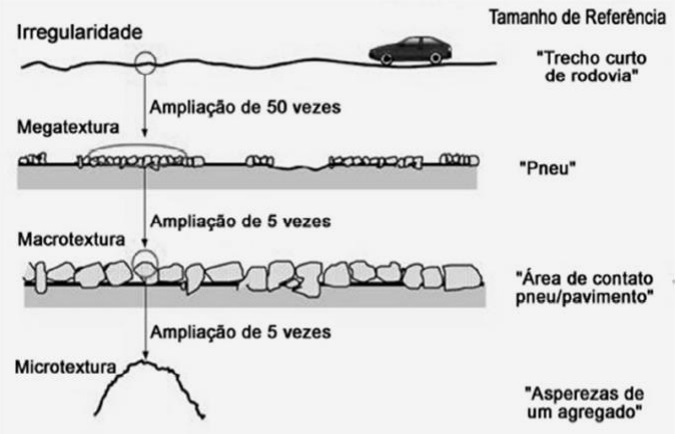
\includegraphics[scale=.70]{figures/tipos_textura.jpg}}\\
\makebox[\width]{Fonte: baseado em \citeonline{kuchiishi}} \label{Fig:tipos_textura}
\end{figure}

\subsection{Rugosidade}
\citeonline{piratelli} define o conceito de rugosidade como o  conjunto de desvios microgeométricos caracterizado pelas pequenas saliências e reentrâncias presentes em uma superfície. Para \apudonline{scheers}{machado} a rugosidade é o conjunto de oscilações de alta freqüência ou de ondas curtas.

Há uma grande similaridade entre as definições de rugosidade e textura, que por vezes chegam a se confundir. Entendemos aqui, a rugosidade como a ocorrência de desvios na superfície e textura como o efeito causado por esses desvios. Os diferentes níveis de rugosidade, corresponderiam portanto, aos diferentes níveis de textura descritos anteriormente, quando os desvios são de ordem de grandezas maiores, caracterizam ondulação e erro de forma (Figura \ref{Fig:rugosidade}). 

\begin{figure}[!ht]
\centering
\caption{Representação dos diferentes níveis de rugosidade.}
{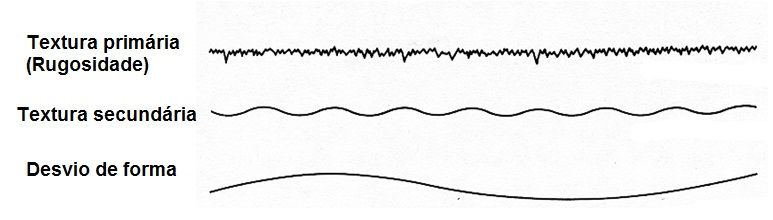
\includegraphics[scale=.70]{figures/rugosidade.jpg}}\\
\makebox[\width] {Fonte: \citeonline{piratelli}} \label{Fig:rugosidade}
\end{figure}

A diferença entre rugosidade, ondulação e erro de forma é baseada no comprimento de onda da superfície analisada ou no espaçamento entre picos \apud{demare}{machado} porém a fronteira entre rugosidade e ondulação é questionável e deve-se especificar numericamente o comprimento da frequência de onda acima ou abaixo do qual uma das componentes da superfície (rugosidade ou ondulação) é eliminada \cite{machado}. 

\subsection{Superfície}
A superfície real de um objeto é definida pela NBR ISO 4287:2002 \nocite{iso4287} como a superfície que limita o corpo e o separa do meio ambiente, ela pode ser representada pela superfície efetiva que é aquela obtida por meio das técnicas de medição. Estes conceitos estão representados na Figura \ref{Fig:superficie}.

\begin{figure}[!ht]
\centering
\caption{Representação das superfícies real e efetiva.} 
{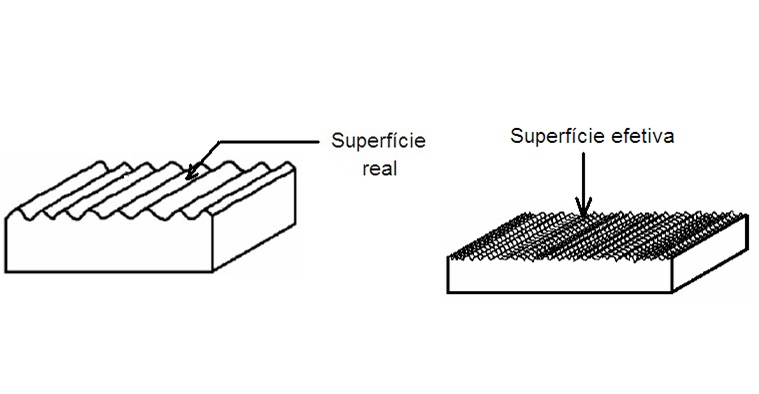
\includegraphics[scale=.65]{figures/superficie.jpg}}\\
\makebox[\width]{Fonte:Adaptado de \citeonline{piratelli}} \label{Fig:superficie}
\end{figure}

\subsection{Perfil de Superfície}
O perfil de superfície é uma representação bidimensional geralmente orientada em um eixo x-y. Ele é resultante da interseção da superfície real e um plano específico NBR ISO 4287:2002 \nocite{iso4287}, como representado na Figura \ref{Fig:perfil_de_superficie}.

\begin{figure}[!ht]
\centering
\caption{Obtenção do perfil de superfície.}
{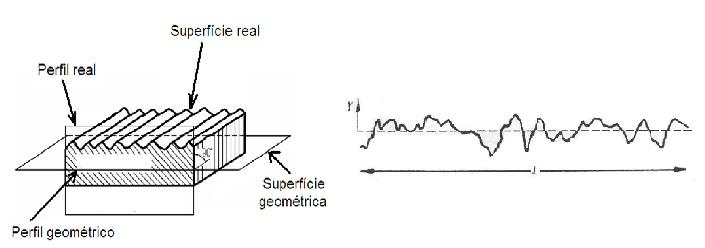
\includegraphics[scale=0.84]{figures/perfil_de_superficie.jpg}}\\
\makebox[\width]{Fonte: Adaptado de \citeonline{piratelli}} \label{Fig:perfil_de_superficie}
\end{figure}

Na prática é usual escolher um plano onde a normal é teoricamente paralela à superfície real e em uma direção apropriada (NBR ISO 4287:2002\nocite{iso4287}).

Para obtenção de um perfil que represente a superfície efetiva existem vários ensaios e equipamentos, contudo alguns métodos como os perfilométricos acabam gerando um perfil composto por todos os níveis de textura, o que nem sempre é prático para a análise que se deseja realizar. Para permitir a separação entre os perfis de rugosidade e de ondulação, a norma propõe uma correção que consiste na filtragem do perfil primário. Assim, temos que a definição do perfil de rugosidade é a seguinte: "perfil derivado do perfil primário pela eliminação dos componentes de comprimento de ondas longas, usando o filtro de perfil $\lambda$c” (NBR ISO 4287:2002). No presente trabalho, esta correção não se fez necessária, uma vez que as dimensões dos corpos de prova utilizados são pequenas, assim os desvios no nível das ondulações e desvios de forma não foram representados.

A partir dos perfis medidos podem ser realizadas caracterizações de parâmetros superficiais específicos \cite{machado}, alguns elementos do perfil devem ser analisados para que se obtenham estes parâmetros. A seguir estão apresentadas as definições compiladas a partir das normas EN ISO 113473-1:1997 \nocite{iso113473} e NBR ISO 4287:2002 \nocite{iso4287}, foram ainda acrescidas as definições de outros autores quando necessário.

\subsection{Linha Média (LM)} 
De acordo com \citeonline{machado} a linha média, identificada na Figura \ref{Fig:lm_e_ca} pode ser determinada de duas maneiras: linha média dos mínimos quadrados, referente ao perfil primário; e linha média filtrada, referente aos perfis de rugosidade e de ondulação.

A primeira definição é apresentada pela NBR ISO 4287:2002\nocite{iso4287}, que define a linha média do perfil como a linha determinada pelo ajuste dos mínimos quadrados à linha da forma nominal do perfil. Ou seja, essa linha acompanha o perfil nominal, de forma que a soma dos quadrados dos desvios do perfil na direção vertical seja minimizado.

A definição da linha média filtrada consta no trabalho de \citeonline{piratelli}, segundo a qual a linha média divide o perfil tal que a soma das áreas acima é igual à soma das áreas abaixo, ao longo do comprimento de medição.

\subsection{Comprimento de Amostragem (L)}
O comprimento de amostragem está identificado na Figura \ref{Fig:lm_e_ca}, a norma o define como sendo o comprimento na direção do eixo X, usado para identificar as irregularidades características do perfil sob avaliação; ou seja, é o comprimento do trecho a ser avaliado.

\begin{figure}[!ht]
\centering
{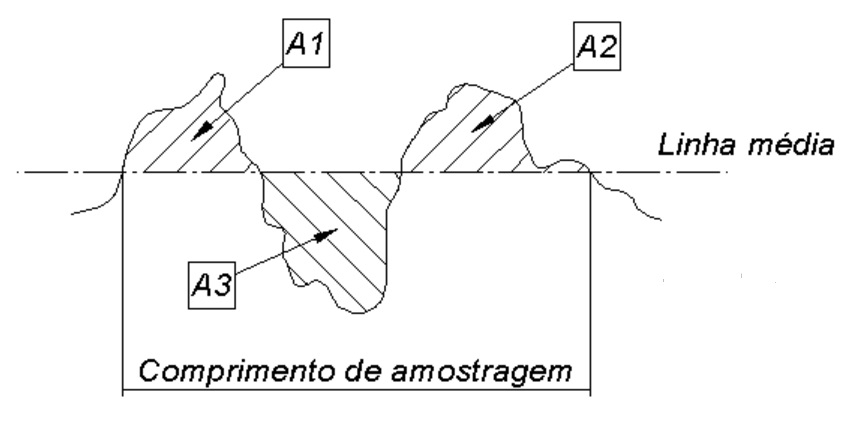
\includegraphics[scale=0.50]{figures/lm_e_ca.jpg}}\\\caption{Representação da linha média e do comprimento de amostragem.}
\makebox[\width]{Fonte: \citeonline{unicamp}} \label{Fig:lm_e_ca}
\end{figure}

\subsection{Altura de pico (Zp) e profundidade do vale (Zv)}
São respectivamente as distância verticais entre o eixo x e o ponto mais alto dos picos do perfil e entre o eixo x e o ponto mais baixo dos vales do perfil. A soma da altura do pico e profundidade do vale é denominada altura de um elemento do perfil (Zt), como representado na Figura \ref{Fig:alturas}.
 Conforme \citeonline{machado}, a avaliação dos picos é importante quando se consideram as propriedades de fricção e desgaste e a interação entre concentração de superfícies.

\begin{figure}[!ht]
\centering
{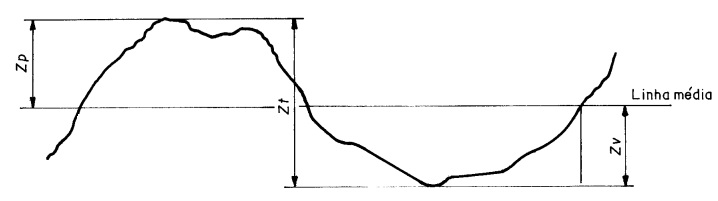
\includegraphics[scale=0.65]{figures/alturas.jpg}}\\\caption{Representação da altura de pico e profundidade de vale.}
\makebox[\width]{Fonte: Adaptado de NBR ISO 4287:2002 \nocite{iso4287}} \label{Fig:alturas}
\end{figure}

\subsection{Altura máxima do pico (Rp) e profundidade máxima de vale do perfil (Rv)}
Os parâmetros de amplitude máxima de picos e vales correspondem ao valor de maior altura de pico (Zp) e de maior profundidade de vale (Zv), no comprimento de amostragem. 
O somatório do mais alto pico (Rp) com o mais profundo vale (Rv) é chamado de amplitude de perfil (Rt). 

\subsection{Rugosidade média ou Amplitude média (Ra)}
O parâmetro de amplitude média de perfil, também é conhecido como média aritmética, média da linha central ou desvio médio aritmético do perfil.
É o valor médio das alturas dos elementos do perfil (Zt) no comprimento de amostragem, obtido pela Equação (\ref{Eq:rugosidademedia}).

\begin{equation}\label{Eq:rugosidademedia}
%
Ra = \frac{\sum Ai}{L}
%
\end{equation}
%

As variáveis $Ai$, $L$ representam respectivamente a área sob a curva entre dois pontos nulos e o comprimento de amostragem, como indicado na Figura \ref{Fig:lm_e_ca}. 

De acordo com \citeonline{machado}, este parâmetro corresponde à área entre o perfil de rugosidade e a linha média, ou ainda, a integral dos valores absolutos das amplitudes do perfil de rugosidade dentro de um comprimento de amostragem.

\subsection{Textura Média do Perfil (MPD)}
É o valor médio da rugosidade do perfil dentro de um comprimento de amostragem. 
Diferença entre a média aritmética de dois picos ($Z_1$ e $Z_2$) e a linha média (LM)\footnote{Observe que a Linha Média não corresponde necessariamente ao eixo coordenado x, quando isso ocorre, o valor de LM na equação é zero.}  em uma distância de 100m. Este parâmetro é obtido pela Equação \ref{Eq:texturamedia}: 

\begin{equation}\label{Eq:texturamedia}
%
MPD = \frac{Z_{1}+Z_{2}}{L} - LM 
%
\end{equation}
%

\section{PARÂMETROS ESTATÍSTICOS
}
O algoritmo utilizado, além de retornar a medida da rugosidade média  e o erro percentual em relação aos dados experimentais, também calcula alguns parâmetros estatísticos descritivos como Desvio padrão, Mediana e Curtose. Estes parâmetros possibilitam a análise quantitativa dos dados.

\subsection{Desvio Médio Quadrático (Rms)}
É uma medida gerada a partir do Desvio Padrão, fornece informações referentes à dispersão dos dados, permitindo analisar  como as alturas se comportam quando distantes da média. É definido como a raiz quadrada da média dos valores das ordenadas $Z(x)$, oferecendo uma medida do desvio padrão dos dados analisados. Este parâmetro é obtido pela Equação \ref{Eq:rms}.

\begin{equation}\label{Eq:rms}
%
Rms = \sqrt\frac{1}{l} \int_0^l Z^2(x)  dx
%
\end{equation}
%

\subsection{Fator de achatamento ou Curtose (Rku)}

A curtose indica a facilidade de se obter valores que não se aproximam da média, representando que a distribuição dos resultados tem achatamento semelhante ao da distribuição normal quando esta medida de dispersão se aproxima de zero \cite{magalhaes}. É definida como o quociente entre o valor médio dos valores das ordenadas Z(x) à quarta potência e o valor de Rms à quarta potência. Este parâmetro é obtido pela Equação \ref{Eq:rku}.

\begin{equation}\label{Eq:rku}
%
Rku = \frac{1}{Rms^4} \bigg[\sqrt\frac{1}{l} \int_0^l Z^4(x)  dx \bigg] 
%
\end{equation}
%

Como enfatizado na NBR ISO 4287:2002\nocite{iso4287}, a curtose é um parâmetro fortemente influenciado por picos isolados ou vales isolados. \citeonline{bernuccipavimentaccao} destaca que, em pavimentos asfálticos, as alturas das asperezas podem não ser normalmente distribuídas, apresentando assim valores distintos de Rku, o que faz com que as superfícies do pavimentos apresentem 
configurações variadas, como mostra a Figura \ref{Fig:curtose}.

\begin{figure}[!ht]
\centering
{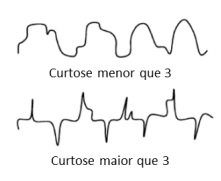
\includegraphics[scale=1.1]{figures/curtose.jpg}}\\
\caption{Influência da curtose na no perfil de superfície.} \makebox[\width]{Fonte:\citeonline{bernuccipavimentaccao}} \label{Fig:curtose}
\end{figure}


\subsection{Mediana (Md)}
A mediana é o valor central de um conjunto de dados, dividindo-o em duas partes iguais. É um parâmetro menos sensível a valores atípicos. Este parâmetro é obtido pela Equação \ref{Eq:md}.

\begin{equation}\label{Eq:md}
%
Md = L_i+\bigg(\frac{\frac{n}{2}-\sum{f'}}{f_{Md}}\bigg) C_{Md}
%
\end{equation}
%

Onde $L_i$ é o limite inferior da classe mediana; $n$ é o total
de frequência; $\sum{f’}$ é soma de todas as frequências das classes inferiores à mediana, $f_{Md}$ é a frequência da classe mediana e $C_{Md}$ é a amplitude da classe mediana.


\section{INFLUÊNCIA DA RUGOSIDADE NO DESEMPENHO DE PAVIMENTOS}
Os desvios na superfície do pavimento são de fundamental importância para garantir condições de segurança e conforto nas rodovias. Para avaliar o estado de conservação dos pavimentos, diversos indicadores foram desenvolvidos ao longo dos anos. O Instituto de Infra-Estruturas Rodoviárias (INIR), em sua disposição técnica \citeonline{azevedo} cita parâmetros de avaliação das características superficiais e estruturais, baseados na rugosidade. São eles:
\begin{itemize}
\item Textura Superficial;
\item Irregularidade Longitudinal;
\item Perfil Transversal. 
\end{itemize}

Cada nível de textura está relacionado à uma propriedade física do pavimento. O atrito no clima seco, por exemplo, é influenciado pelos níveis de macrotextura e microtextura, ou seja, por rugosidades compreendidas no intervalo  entre 1$\mu$m e 10mm, como representado na Figura \ref{Fig:influencia}.


\begin{figure}[!ht]
\centering
{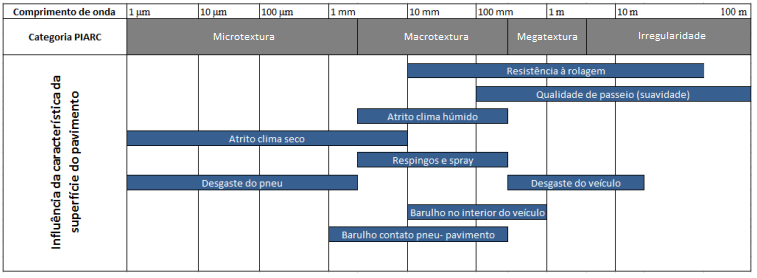
\includegraphics[scale=0.8]{figures/influencia.jpg}}\\
\caption{Influência das características da superfície no desempenho dos pavimentos.} 
\makebox[\width]{Fonte: \citeonline{bitelli}} \label{Fig:influencia}
\end{figure}

A macrotextura garante a resistência à derrapagem, principalmente em velocidades elevadas ou quando o pavimento encontra-se molhado, contribui também para melhorar a visibilidade em condições de pista molhada, elimina ou atenua a reflexão da luz melhorando a percepção das marcas de sinalização horizontal e reduz o barulho gerado pelo contato entre pneu e pavimento. A microtextura, ou a aspereza do pavimento, por sua vez, é necessária para se conseguir uma boa aderência a baixas velocidades e no pavimento seco, além de regular o desgaste dos pneus.

A megatextura e a irregularidade superficial são características indesejáveis, de qualquer ponto de vista. Incidem negativamente sobre o conforto e aumentam o ruído de rolamento, os gastos com a manutenção dos veículos e os gastos com a conservação do pavimento \cite{azevedo}.

Observa-se que os níveis que predominantemente afetam o atrito são a microtextura e a macrotextura, por isso, essas características são os principais objetos de estudos que relacionam a rugosidade e o desempenho de pavimentos. Dentre eles podemos citar o de \citeonline{boscaino}, que correlacionou propriedades de superfícies asfálticas, como a textura superficial, com a absorção acústica dos pavimentos. O mesmo tema foi abordado por \citeonline{callai}, que realizou um estudo de caso na cidade de São Paulo, analisando a emissão de ruído em diferentes tipos de revestimento. 

Outro estudo de caso foi conduzido por \citeonline{pulugurtha} na Carolina do Norte, Estados Unidos. Ele associou o efeito da macrotextura com o aumento da segurança da pista, provando uma forte relação entre ambos. No Brasil, estudos semelhantes foram desenvolvidos, como o de \citeonline{dasilva}, em São Paulo, o qual avaliou a redução de acidentes na rodovia Fernão Dias com a troca do revestimento da pista. Os resultados demonstraram que após a substituição do Concreto Asfáltico, que apresenta uma textura fina, pelo Microrrevestimento cuja textura varia de média a grossa, houve uma significativa redução dos acidentes.  

Segundo \citeonline{bitelli}, os indicadores de performance são, em geral, relacionados às diferentes condições de medição (velocidade de deslizamento, estado da superfície, ângulo entre as direções de deslocamento e os pneus, etc.), cada uma possui uma ténica de medição específica, geralmente regulmentada por padrões nacionais ou internacionais. Dentre os ensaios e aparelhos criados para aferição dos parâmetros superficias de um pavimento, classificam-se os métodos em perfilométricos ou estáticos. 

Nas medições estáticas, destaca-se o Ensaio de Mancha de Areia, que mede a rugosidade em nível de macrotextura. A eficiência deste ensaio foi objeto de pesquisa como \citeonline{specht} e  \citeonline{kuchiishi}. Outro ensaio é o chamado Pêndulo Britânico, destinado à medição da rugosidade à nível da microtextura como estudado por \citeonline{lee}. Há ainda pesquisas que utilizam processamento de imagens como método de caracterização da textura \cite{slimane}, \cite{khoudeirs}.

Em relação aos métodos perfilométricos há diversos tipos de equipamentos disponíveis. No nosso país, os equipamentos empregados em maior escala são os do tipo resposta, que fornecem um somatório de desvios do eixo de um veículo em relação à suspensão ou até mesmo por meio de levantamentos topográficos. Um destes aparelhos é o chamado rugosímetro BPR, porém ele apresentou falhas como indicado por \citeonline{perera}, uma vez que estava sujeito à variações de temperatura além de produzir algumas frequências resssoantes que provocaram resultados incorretos. O   Maysmeter, foi outro equipamento amplamente utilizado entre os anos de 1960 e 1980, inclusive no Brasil, pelo antigo DNER (Departamento Nacional de Estradas de Rodagem). Contudo, este acabou sendo substituído no país pelo perfilômetro inercial desenvolvido em parceria pelo IPR (Instituto de Pesquisas Rodoviárias) e pela USP (Universidade de São Paulo). Este equipamento consiste em um veículo de passeio no qual são acoplados um sensor de deslocamentos verticais e um quantificador de irregularidade, o desenvolvimento e utilização deste equipamento foi descrito por \citeonline{barella}. 

\section{EMPREGO DE MÉTODOS DE ESCANEAMENTO PARA ANÁLISE DE PAVIMENTO}

Nos últimos anos, os dispositivos de escaneamento a laser têm sido difundidos e se tornado mais acessíveis, assim, diversas aplicações para este equipamento vem sendo estudadas. O sistema de escaneamento com uso de laser é um dos tipos de técnicas denominadas LiDAR (Light Detection and Ranging). Nesta classificação podemos discernir ainda os escaneamentos dos tipos ALS, TLS e MLS, respectivamente: escaneamento aéreo a laser, escaneamento terrestre a laser e escaneamento móvel a laser, em tradução livre. Dentre os usos já explorados para essa tecnologia, podemos citar estudos nas áreas de: gerenciamento florestal \cite{means}, \cite{giongo}, mapeamento de regiões \cite{schwarz} e na indústria automotiva \cite{rasshofer}.

A caracterização da textura superficial de pavimentos por meio de escaneamento tridimensional conforme proposto neste trabalho, já foi realizada por outros autores como \citeonline{bitelli}, cujo procedimento foi uma das referências para esta pesquisa. Ressalta-se dentre as similaridades, o uso de corpos de prova extraídos em campo, além de outros moldados in-loco e também o uso do mesmo equipamento, o Next Engine® laser scanner.  Os parâmetros obtidos foram agrupados em duas classes: a primeira leva em consideração parâmetros “geométricos” relacionados à morfologia da amostra analisada; a segunda classe inclui indicadores estatísticos do desempenho(...), que analisam os aspectos da interação entre o pneu e a superfície do pavimento \cite{bitelli}.

A conclusão do experimento de \citeonline{bitelli} foi bastante satisfatória, a análise dos diferentes tipos de pavimento: DGAC (concreto asfáltico de graduação densa); SMA (concreto asfalto de graduação descontínua), e OGAC (concreto asfáltico de graduação aberta); correspondeu às expectativas, caracterizando o DGAC como um pavimento menos rugoso e o OGAC como o de maior rugosidade.

\citeonline{sengoz} utilizaram o scanner Metris Model Maker D100 3D e comapararam os resultados com o tradicional ensaio de Mancha de Areia. O equipamento utilizado foi montado sobre uma base móvel e conectado à um computador para realizar a coleta de dados. Para análise dos resultados, foi traçada uma curva MPD (profundidade média do perfil) versus MTD (profundidade média da textura) e foi encontrado o coeficiente de correlação bastante elevado de $R^2 = 0.97$. Baseando-se nas conclusões da PIARC (congresso internacional sobre rodovias, produzido pela \emph{World Road Association}) de que o melhor parâmetros para determinação do coeficiente de atrito seria o MPD,  eles verificam que o a o partir do MTD pode-se também prever de forma satisfatória este coeficiente.

\citeonline{pratico} conduziram outro estudo focado na relação entre no MPD e no MTD. Porém, este utilizou um equipamento de escaneamento bidimensional. Foram considerados os seguintes tipos de revestimentos: DGFC (revestimento de graduação densa), SMA (revestimento de graduação descontínua), OGFC (revestimento de graduação aberta) e PEM (mistura porosa). Verificou-se que para rugosidades inferiores a 1,5mm, uma função linear era bem representativa. Contudo, para valores acima de 1,5mm, houve uma visível divergência de resultados. O estudo concluiu que a correlação entre o MPT e a medida do ensaio de mancha de areia apresenta algumas complexidades e que a divergência encontrada baseia-se essencialmente no fato de que o ensaio é tridimensional, enquanto o escaneamento realizado era bidimensional. Para associar os resultados, foi adaptada uma curva e apesar das ressalvas, a conclusão deste estudo foi um modelo satisfatório para correlacionar as grandezas, e que representa uma boa parte dos pavimentos asfaltos em uso.

\citeonline{celko} em sua pesquisa, medem a macrotextura e realizam uma comparação minuciosa entre medições feitas a partir do Método Volumétrico (MTD) e do perfilômetro GE (MPD) com medições do ZScanner\textsuperscript{\textregistered} 800, também é feita a medição e comparação do coeficiente de atrito por diferentes métodos. As medições obtidas pelo scanner são processadas por meio de um algoritmo desenvolvido no MATLAB\textsuperscript{\textregistered}. É interessante ressaltar que em todas as comparações foram obtidos resultados razoalmente próximos, principalmente, entre os valores do scanner 3D e do método volumétrico, para a qual foi obtido o coeficiente de correlação $R^2 = 0.94$. A diferença entre o método aqui apresentado e o proposto por \citeonline {celko} consiste principalmente no fato de que o foi utilizado um scanner fixo, sendo necessária a extração de amostras para que fosse possível realizar o escaneamento. Ainda assim, espera-se que seja possível comparar os resultados como forma de validação do método.  


\chapter{OBJETIVOS}\label{CAP3}
Esta seção abordará os objetivos gerais e específicos deste trabalho.
\section{OBJETIVO GERAL}
Este trabalho visa buscar um conhecimento amplo de toda a arquitetura automotiva relacionada aos seus sistemas embarcados, e como esses sistemas se comunicam entre si. Além deste estudo, o trabalho propõe também: buscar conhecimento técnico sobre sistemas computadorizados de baixo custo, com a finalidade de poder interagir com a rede veicular interna; adquirir aprendizado sobre a arquitetura, a infraestrutura e o armazenamento web utilizando serviços de computação em nuvem, como a \textit{Amazom Web Services (AWS)}, a fim de manter os dados que foram coletados e enviados através de um dispositivo de baixo custo.

Desta forma, este trabalho propõe a implementação de um sistema computadorizado de baixo custo que se conecte e interaja com a rede interna do automóvel – sendo possível coletar algumas informações presentes nesta rede – e que transmita os dados para um serviço de computação em nuvem com o objetivo de manter essas informações para uma futura análise e ou alguma aplicação envolvendo a Internet das Coisas.

\section{OBJETIVOS ESPECÍFICOS}
Para alcançar o sucesso deste trabalho, o objetivo geral foi dividido em alguns objetivos específicos que estão listados abaixo:
\begin{itemize}
\item Estudar a arquitetura dos sistemas embarcados presentes nos automóveis;
\item Levantar e estudar os protocolos de comunicação utilizados pela rede interna automotiva;
\item Pesquisar por sistemas computadorizados de baixo custo e estudo da arquitetura;
\item Analisar a viabilidade de integração de um sistema computadorizado de baixo custo à rede veicular interna;
\item Desenvolver um software embarcado responsável por realizar a conexão e interação do dispositivo computadorizado com a rede interna do automóvel;
\item Estudar a arquitetura e infraestrutura dos serviços de computação em nuvem;
\item Implementar um banco de dados utilizando uma infraestrutura de computação em nuvem;
\item Integrar o software com o banco de dados para armazenar as informações coletadas;
\item Desenvolver uma página web para consultar e disponibilizar as informações contidas no banco de dados.
\end{itemize}


\chapter{FUNDAMENTAÇÃO TEÓRICA}\label{CAP4}
Nesta seção serão abordados todos os assuntos que foram estudados para a contrução deste trabalho.
\section{SISTEMAS E SOFTWARE EMBARCADOS}\label{secaosistemasembarcados}
A definição de sistemas embarcados, segundo \citeonline{leeseshia}, são sistemas computacionais pouco perceptíveis, que geralmente são responsáveis por executar pequenas atividades de forma autônoma, como controlar os robôs da linha de produção de uma fábrica ou gerenciar os semáforos de uma cidade. De acordo com \citeonline{carrowagner} os sistemas computacionais embarcados estão presentes em boa parte das atividades humanas, passando desde o sistema de transporte até os eletrodomésticos de uma residência. Baseado nestes argumentos, sistemas embarcados são todos os dispositivos com poder de processamento, memória e fontes de energia limitados \cite{leeseshia}, que podem se integrar com o meio físico.

\citeonline{leeseshia} ainda reforçam que os programas que são executados nestes dispositivos são chamados de software embarcado. \apudonline{gill}{leeseshia} da \textit{National Science Foundation in the US} cria o termo sistemas ciberfísicos \textit{(Cyber-Physical Systems – CPS)} para se referir à integração da computação com processos físicos. Observa-se aqui uma outra definição para sistemas embarcados. No \textit{CPS}, os sistemas informatizados monitoram e controlam os processos físicos geralmente executando instruções dentro de loops. \citeonline{leeseshia} ainda reforça que é importante compreender a dinâmica dos sistemas computacionais junto com os processos físicos. Por lidar diretamente com o mundo físico, o tempo necessário para executar uma tarefa, nos sistemas ciberfísicos, pode ser fundamental para o correto funcionamento do sistema. A passagem do tempo no mundo físico é algo crítico, ao contrário do mundo cibernético.

Enquanto no processo físico existem diversas coisas acontecendo concorrentemente (ao mesmo tempo), nos processos de software as atividades acontecem em etapas sequenciais. \citeonline{leeseshia} afirmam que o maior desafio técnico na concepção e análise do software embarcado se deriva da necessidade de unir a semântica sequencial do mundo lógico com a realidade concorrente do mundo físico.

\section{SISTEMAS DISTRIBUÍDOS}\label{secaosistemasdistribuidos}
Um sistema distribuído, segundo \citeonline{tanenbaum}, é um conjunto de computadores independentes que que se apresentam ao usuário final como um único sistema coerente. De maneira genérica, a arquitetura de um sistema distribuído é composto por diversos itens de hardware que atuam de forma autônoma - geralmente processando informações específicas - mas que se comunicam entre si caracterizando-se como apenas um único hardware responsável pelo sistema como um todo. O autor ainda reforça que as pessoas ou usuários acham que estão interagindo com um sistema apenas, e não com um conjunto de sistemas. Contudo, para garantir a operação de todo este conjunto, é preciso que haja a colaboração de todos os componentes e dispositivos que fazem parte do sistema. A essência do sistema distribuído está em estabelecer essa colaboração.

Não é estabelecido nenhum padrão ou premissa relacionado ao tipo de hardware que irá compor o sistema. \citeonline{tanenbaum} ainda afirma que esses dispositivos podem variar desde computadores centrais até pequenos nós em redes de sensores. Também não existe premissa com relação ao modo com que os dispositivos se interligam. A característica principal dos sistemas distribuídos está em ocultar boa parte da comunicação interna deste conjunto ao usuário. \citeonline{tanenbaum} define ainda quatro metas que devem ser cumpridas para que o esforço necessário para a construção de um sistema distribuído seja válida: o sistema deve oferecer fácil acesso a seus recursos; deve ocultar razoavelmente bem o fato de que os recursos são distribuídos por uma rede; deve ser aberto e deve permitir a sua expansão.


\section{ARQUITETURA DO SISTEMA AUTOMOTIVO}
Para compreender como funciona a comunicação interna do veículo, é necessário antes saber como o sistema está estruturado, quais dispositivos e controladores utilizados, qual a arquitetura adotada e quais protocolos estão implementados. Para \citeonline{navetsimonotlion}, os fabricantes de automóveis diferenciam em várias categorias os eletrônicos embarcados que um carro possui. Eles utilizam essas categorias para agrupar sistemas mecânicos e ou eletrônicos de acordo com as suas funcionalidades.

\subsection{CATEGORIAS FUNCIONAIS DOS SISTEMAS EMBARCADOS AUTOMOTIVOS}
Historicamente, segundo os autores, existem cinco categorias de sistemas embarcados: \textit{Power Train}, \textit{Chassis}, \textit{Body}, \textit{HMI} e \textit{Telematics}. A categoria \textit{Power Train} fazem parte todos os sistemas que participam da propulsão longitudinal do veículo, incluindo o motor, a transmissão e todos os componentes que dão apoio para esta função. A categoria \textit{Chassis} se refere às quatro rodas e à sua posição relativa de movimento. Nesta categoria os principais sistemas são o de freios e direção. Dentro da categoria \textit{Body} estão presentes as entidades que não pertencem à dinâmica do veículo, mas que auxiliam o motorista, como o airbag, limpadores, iluminação, vidros, ar condicionado, assentos, etc. Já a categoria \textit{HMI} inclui o equipamento que permite a troca de informações entre os sistemas eletrônicos e o motorista do veículo. Por fim, a categoria \textit{Telematics} está relacionado à componentes que permitem a troca de informações do veículo com o mundo exterior, como rádio, sistemas de navegação, GPS, entre outros. \citeonline{navetsimonotlion} ainda ressaltam que cada categoria do sistema eletrônico possui características bem diferentes, o que faz com que cada dispositivo tenha um requisito ou uma restrição bem definida. A Figura \ref{Fig:categorias_sistemas_embarcados} ilustra a divisão funcional dos sistemas pelas categorias.

\begin{figure}[!ht]
\centering
\caption{Representação das cinco categorias funcionais.} 
{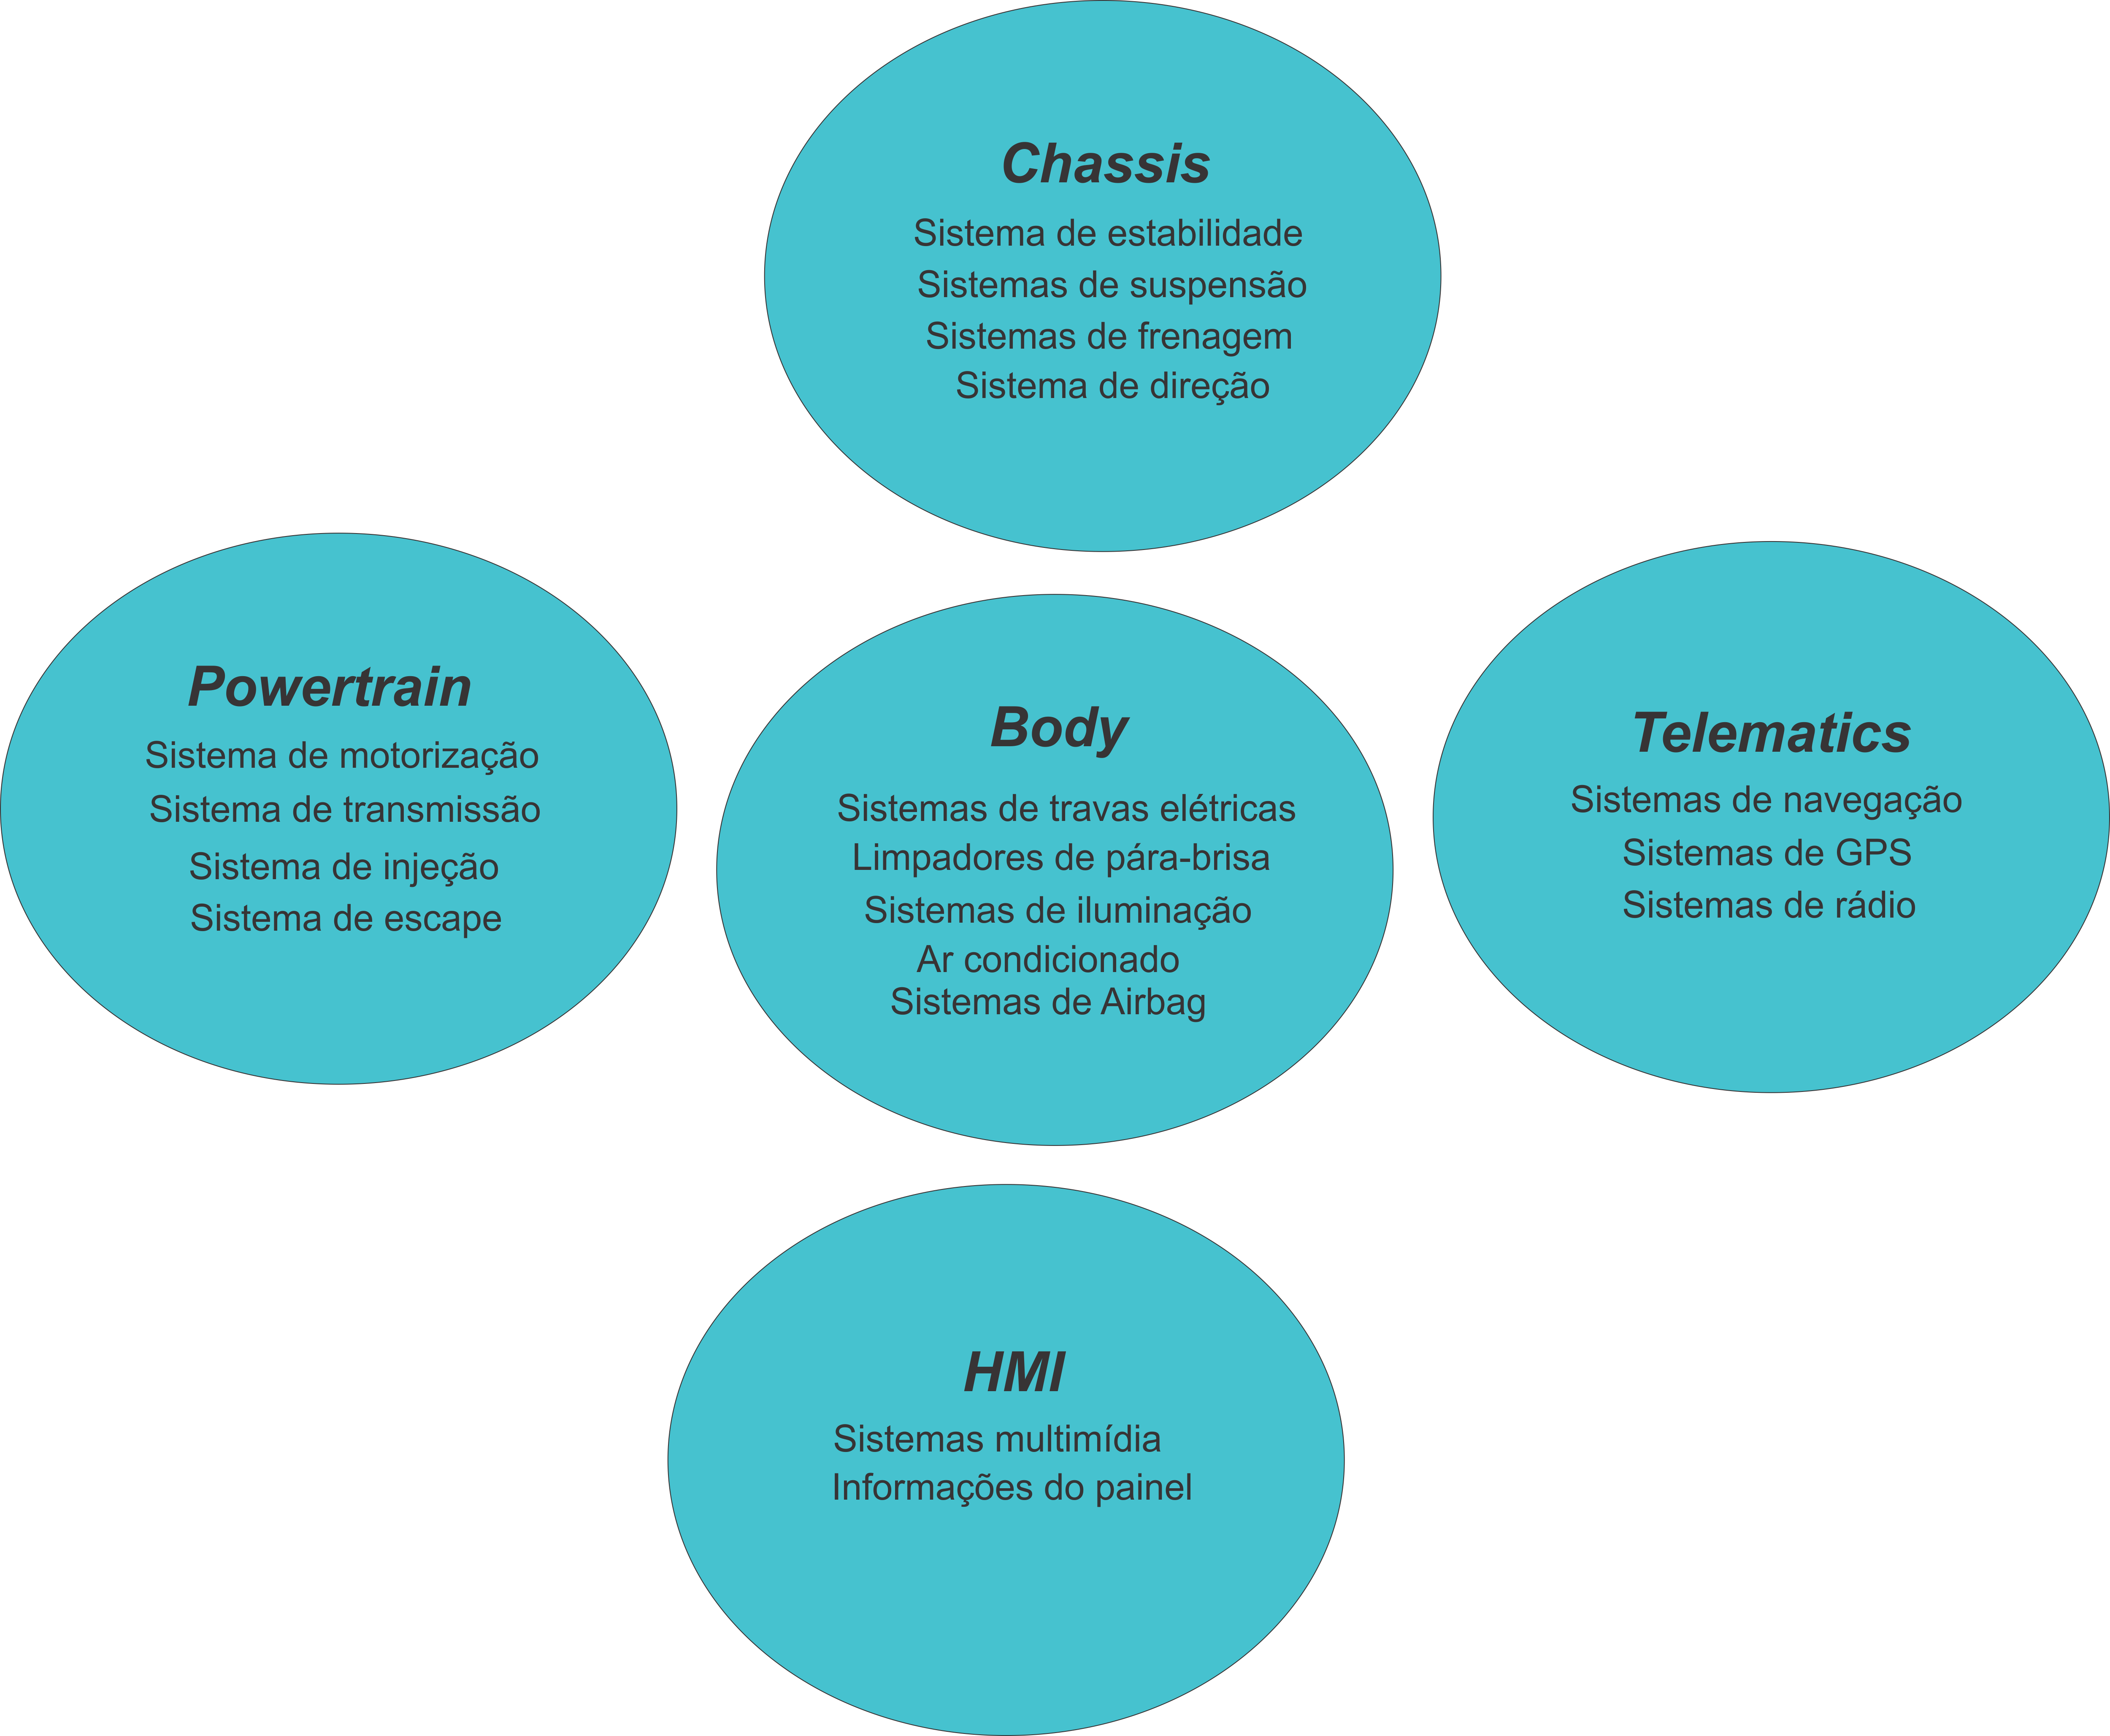
\includegraphics[scale=.31]{imagens/categoriaFuncionalSistemasEmbarcados.png}}\\
\makebox[\width]{Fonte: baseado em \citeonline{navetsimonotlion}} \label{Fig:categorias_sistemas_embarcados}
\end{figure}


\begin{itemize}
\item{Categoria \textit{Power Train}:}
Além de controlar a velocidade do motor, atuando de acordo com as intervenções do motorista no pedal, o controlador pode também, atuar de acordo com fatores naturais, como a temperatura do ar ou o nível de oxigênio, ou atuar de acordo com os distúrbios ambientais, como a poluição dos gases de escape ou o ruído. Ainda segundo \citeonline{navetsimonotlion}, o controlador é projetado para otimizar alguns parâmetros. O parâmetro mais comum a ser controlado é a quantidade de combustível que deve ser injetado para combustão de acordo com a rotação do motor e a posição do pedal do acelerador. Observa-se que nesta categoria estão presentes todos os dispositivos que auxiliam no gerenciamento do motor, tanto de forma direta quanto indireta.

\item{Categoria \textit{Chassis}:}
Nesta categoria, existem sistemas responsáveis por gerenciar a interação do veículo com a estrada. O objetivo destes sistemas é controlar o automóvel de acordo com as solicitações do motorista, como frenagem ou aceleração, considerando também o perfil da via ou as condições ambientais, visando sempre o conforto e a segurança dos passageiros. \citeonline{navetsimonotlion} ainda reforça que esses sistemas devem ser de alta qualidade, como qualquer sistema crítico. Os sistemas mais comuns são o de frenagem (ABS) e o controle automático de estabilidade (ASC).

\item{Categoria \textit{Body}:}
Limpadores de para-brisa, luzes, portas e janelas e outros itens são controlados por sistemas pertencentes a esta categoria. Estes, por sua vez, não estão sujeitos a restrições de desempenho rigorosas, e do pondo de vista de segurança, segundo os autores, não representam uma parte crítica do sistema. Entretanto, existem certas funções, como controlar o acesso ao veículo, que deve respeitar as dificuldades em tempo real.

\item{Categoria \textit{HMI}:}
Os sistemas presentes nesta categoria, em geral, permite a interação do motorista com diversas funções integradas no veículo. Uma das funções é exibir o estado atual do veículo, como velocidade, rotação do motor e temperatura, por exemplo, ou também mostrar o estado de algum dispositivo multimídia.

\item{Categoria \textit{Telematics}:}
Esta categoria, ainda segundo \citeonline{navetsimonotlion}, inclui sistemas que suportam trocas de informações entre infra-estruturas viárias e rodoviárias. Um exemplo está relacionado com a cobrança automática de pedágios. Para os autores, em um futuro próximo, esta categoria permitirá otimizar o uso rodoviário através da gestão do tráfego a fim de evitar congestionamentos.
\end{itemize}

A divisão dos sistemas por categoria engloba dispositivos de acordo com suas semelhanças funcionais. Logo, se um conjunto eletrônico, mesmo que sejam diferentes, seguirem um determinado requisito comum à uma categoria, estes pertencerão à esta. Entretanto, os sistemas eletrônicos, mesmo pertencendo à uma categoria distinta, não são impedidos de se comunicarem entre si. Segundo o exemplo de \citeonline{navetsimonotlion}, as informações como a rotação do motor, temperatura ou a velocidade fazem parte do gerenciamento do motor, e logo pertencem à categoria \textit{power train}, mas são transmitidas desta para a categoria \textit{HMI}, para exibir as informações do veículo ao motorista no painel de instruções (Figura \ref{Fig:comunicacao_categorias_sistemas_embarcados}).

\begin{figure}[!ht]
\centering
\caption{Representação do monitoramento de RPM e a comunicação entre as categorias.} 
{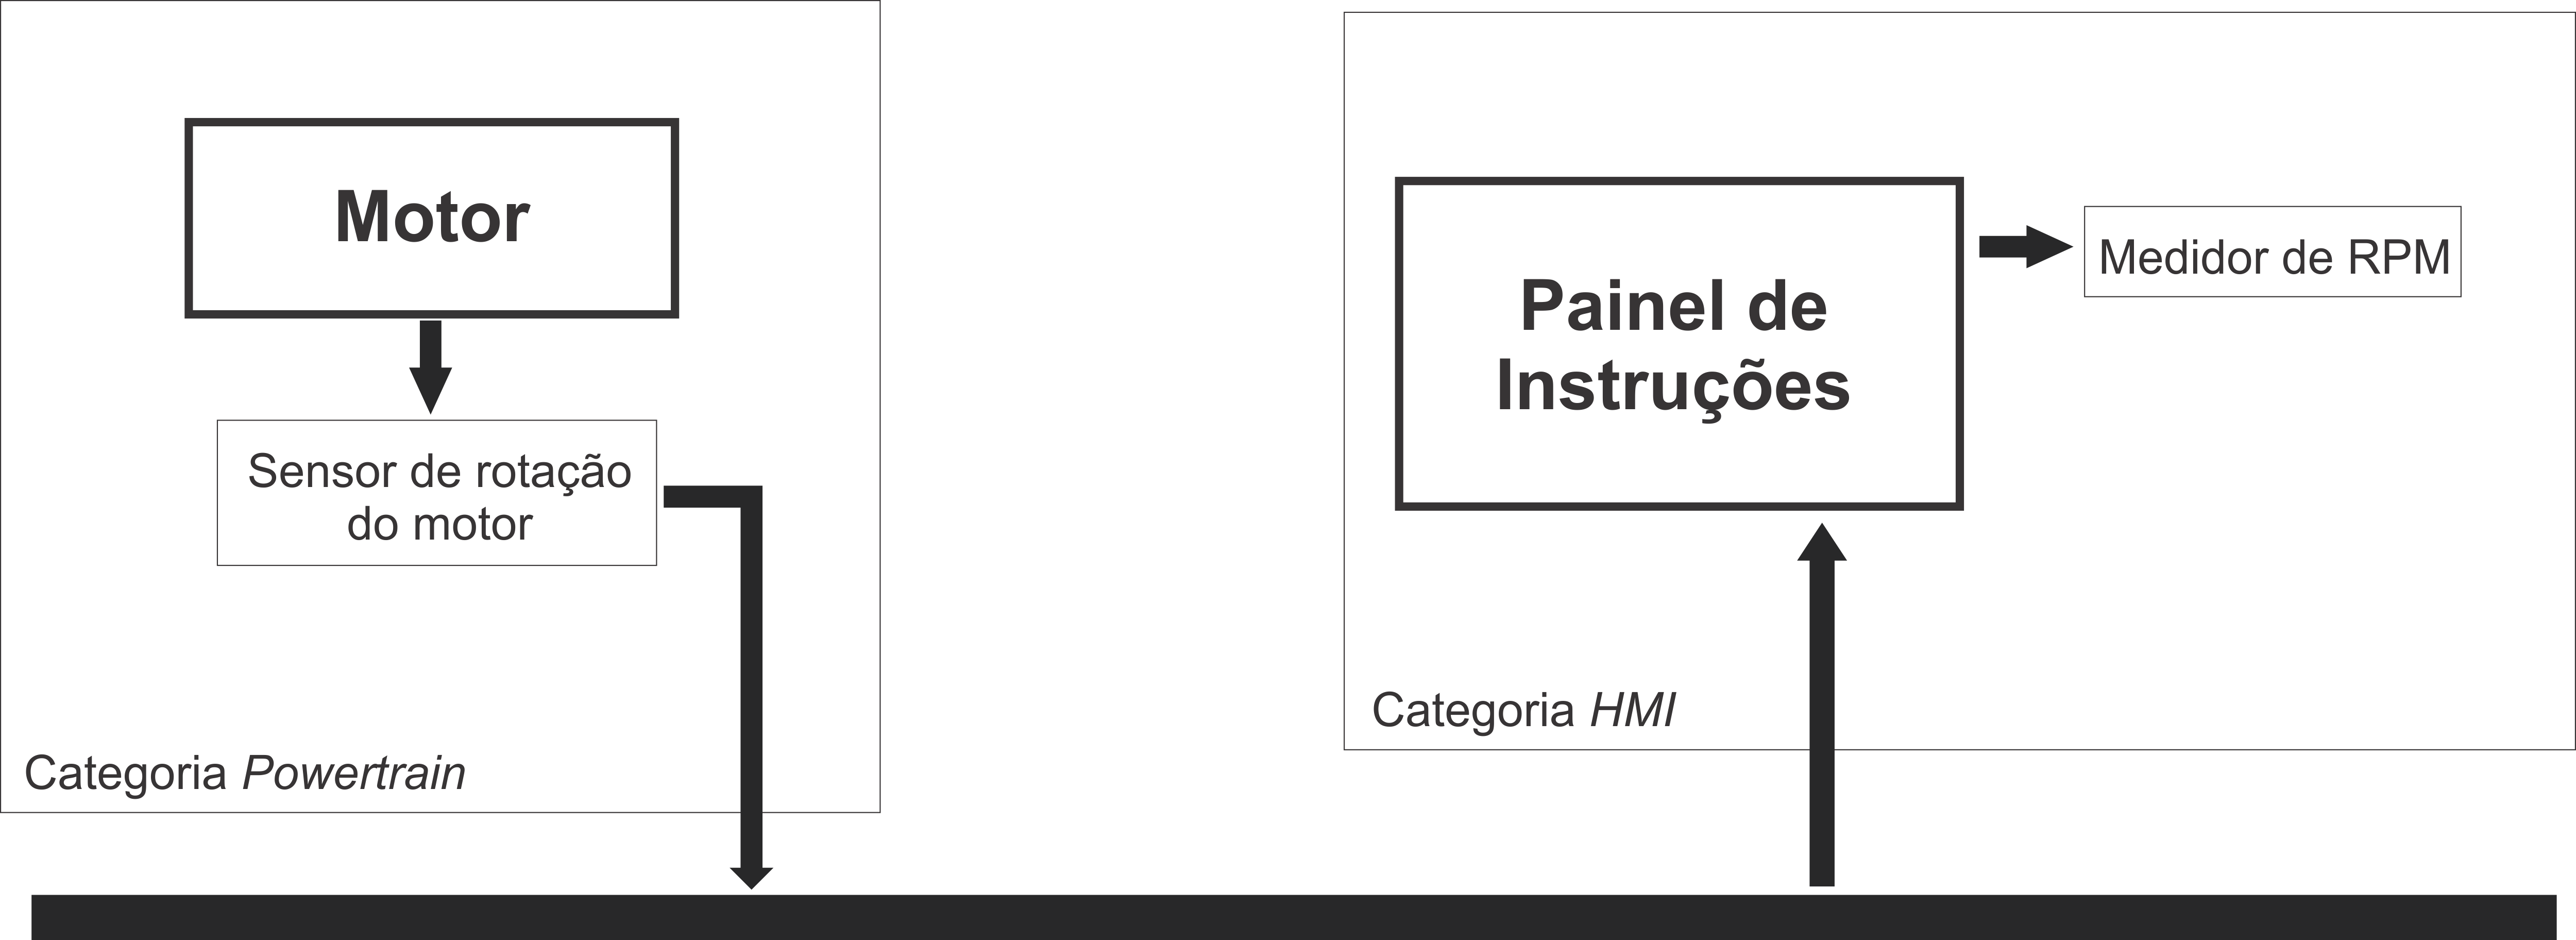
\includegraphics[scale=.37]{imagens/intercomunicacaoEntreCategorias.png}}\\
\makebox[\width]{Fonte: baseado em \citeonline{navetsimonotlion}} \label{Fig:comunicacao_categorias_sistemas_embarcados}
\end{figure}

Analisando o funcionamento destes sistemas eletrônicos, eles são caracterizados como sistemas embarcados automotivos pelo fato de possuírem uma forte interação com o mundo físico, conforme a definição de sistemas embarcados explorado na seção \ref{secaosistemasembarcados}. Para interagir com o mundo físico, estes sistemas fazem o uso de outros dispositivos conhecidos como sensores e atuadores. Segundo \citeonline{leeseshia}, um sensor mede uma quantidade física, enquanto o atuador altera a quantidade física. Eles ainda complementam que estes dispositivos conectam o mundo cibernético com o mundo físico. Em outras palavras, um sensor obtém os dados de uma leitura, e o atuador realiza uma ação que foi passado a ele. Em um automóvel existem diversos sensores espalhados por sua estrutura e que monitoram diversos aspectos físicos do veículo, como aceleração lateral, velocidade e tração individual das rodas, monitorando a estabilidade do carro durante o percurso \cite{navetsimonotlion}. O autor ainda complementa que quando uma correção precisa ser aplicada nesta situação, as rodas dianteiras ou traseiras podem frear individualmente e com intensidades diferentes, ou atuar na redução da potência do motor. Percebe-se neste exemplo a ação dos atuadores no meio físico. A Figura \ref{Fig:relacao_sensor_atuador} representa a influência destes dispositivos no meio físico.

\begin{figure}[!ht]
\centering
\caption{Representação da atuação dos sensores e atuadores.} 
{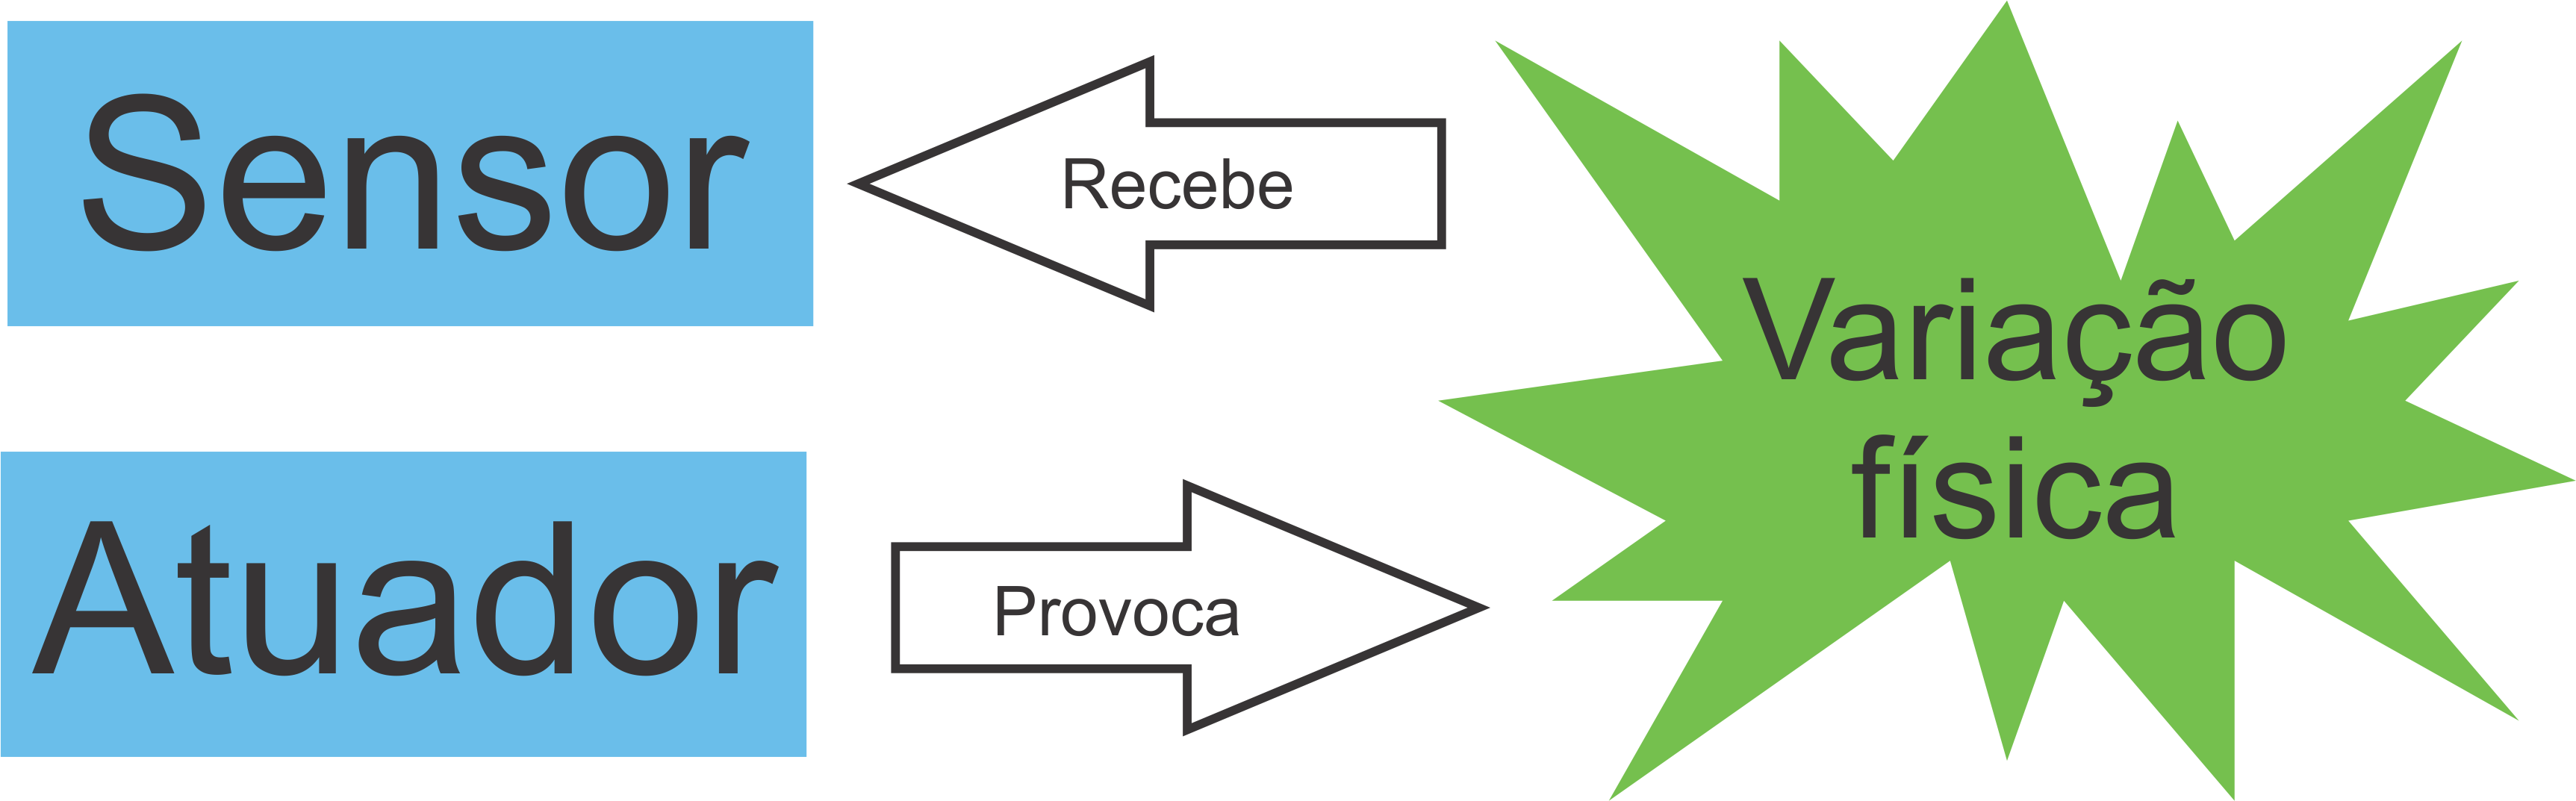
\includegraphics[scale=.29]{imagens/relacaoSensorAtuador.png}}\\
\makebox[\width]{Fonte: baseado em \citeonline{leeseshia}} \label{Fig:relacao_sensor_atuador}
\end{figure}

Analisando-se também a forma como esses dispositivos trocam informações uns com os outros, percebe-se que está presente o conceito de sistemas distribuídos, conforme apresentado na seção \ref{secaosistemasdistribuidos}. Um exemplo desse conceito no cenário automotivo é mencionado por \citeonline{navetsimonotlion}, que está relacionado com a funcionalidade de piloto automático \textit{(cruise control)} presente em alguns modelos de veículos. Para que esse sistema funcione perfeitamente, segundo os autores, é necessário a troca de dados de vários sensores que podem pertencer a categorias funcionais distintas. A função de piloto automático tem a responsabilidade central de processar esses dados vindos de diversas origens e enviar as respostas a vários outros dispositivos de saída para cumprir seu objetivo.

Desde a década de 70, como aponta \citeonline{navetsimonotlion}, houve um aumento muito grande no número de sistemas que passaram a substituir os que eram puramente mecânicos ou hidráulicos. O desempenho e confiabilidade desses componentes de hardware que passaram a integrar o automóvel permite a execução de funções complexas, aumentando o conforto e a segurança dos ocupantes do veículo. A arquitetura de hardware de um automóvel não é composta somente de sensores, atuadores, controladores e links de comunicação que permite a interconexão dos componentes, mas também de dispositivos conhecidos como \textit{ECUs}.

\subsection{\textit{ECU (ELETRONIC CONTROL UNIT)}}
Um veículo possui alguns controladores eletrônicos, que para \citeonline{smith}, são chamados de dispositivos informatizados que passam por diversos nomes diferentes, como Unidade de Controle Eletrônico \textit{(Eletronic Control Unit - ECU)}, Unidade de Controle do Motor \textit{(Engine Control Unit – ECU)}, Unidade de Controle de Transmissão \textit{(Transmission Control Unit – TCU)} ou ainda Módulo de Controle de Transmissão \textit{(Transmission Control Module – TCM)}. O autor ainda destaca que esses termos na teoria podem ter significados específicos em uma determinada configuração, mas na prática acaba utilizando-se o termo \textit{ECU} que é comum a eles. Isso porque independente do tipo de controlador eletrônico, eles acabam executando as mesmas funções, ou funções extremamente semelhantes. \citeonline{navetsimonotlion} afirmam que um dos principais propósitos dos sistemas eletrônicos é auxiliar o condutor a controlar o veículo. Segundo eles, a \textit{ECU} autônoma é um subsistema composto por um microcontrolador e um conjunto de sensores e atuadores associados. Os autores também trazem a ideia de que as \textit{ECUs} podem aprimorar a ação dos atuadores, indo muito além da capacidade humana sobre eles. A Figura \ref{Fig:ecu} apresenta a foto de uma \textit{ECU}.

\begin{figure}[!ht]
\centering
\caption{Foto de uma \textit{ECU}.} 
{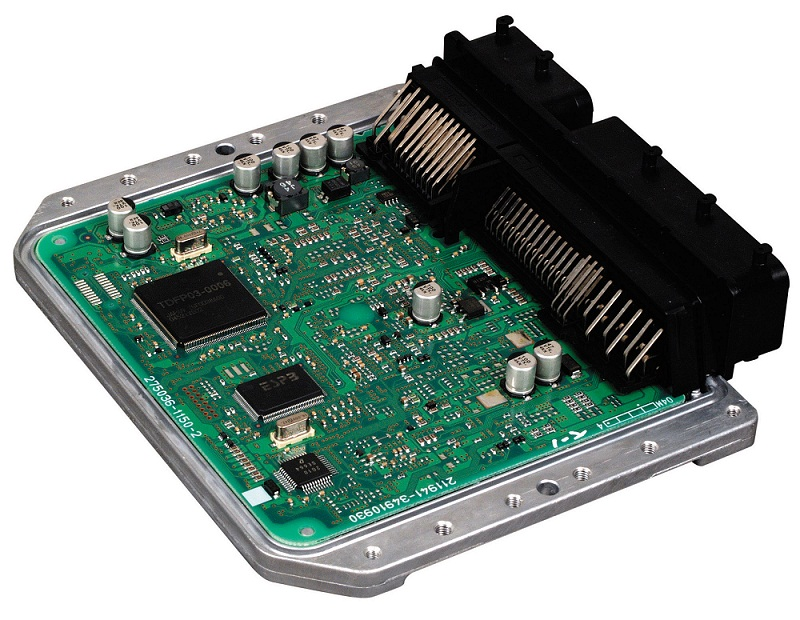
\includegraphics[scale=1.3]{imagens/ecu1.jpg}}\\
\makebox[\width]{Fonte: imagem extraída do site http://carrosinfoco.com.br/wp-content/uploads/2012/07/ecu1.jpg} \label{Fig:ecu}
\end{figure}

Em outras palavras, a \textit{ECU}, de forma geral, é um dispositivo capaz de processar as informações recebidas pelos sensores dos veículos, e gerar uma resposta para a ação dos atuadores, conforme está representado na Figura \ref{Fig:relacao_ecu_sensor_atuador}. Como a \textit{ECU} faz parte de um sistema embarcado, sua memória e capacidade de processamento são limitadas assim como qualquer dispositivo embarcado, conforme abordado na seção \ref{secaosistemasembarcados}. Entretanto, as \textit{ECUs} são destinadas a executar determinadas tarefas em específico, de modo que o desempenho do sistema como um todo não seja afetado pela limitação de hardware do dispositivo.

\begin{figure}[!ht]
\centering
\caption{Diagrama da comunicação entre \textit{ECU}, sensor e atuador.} 
{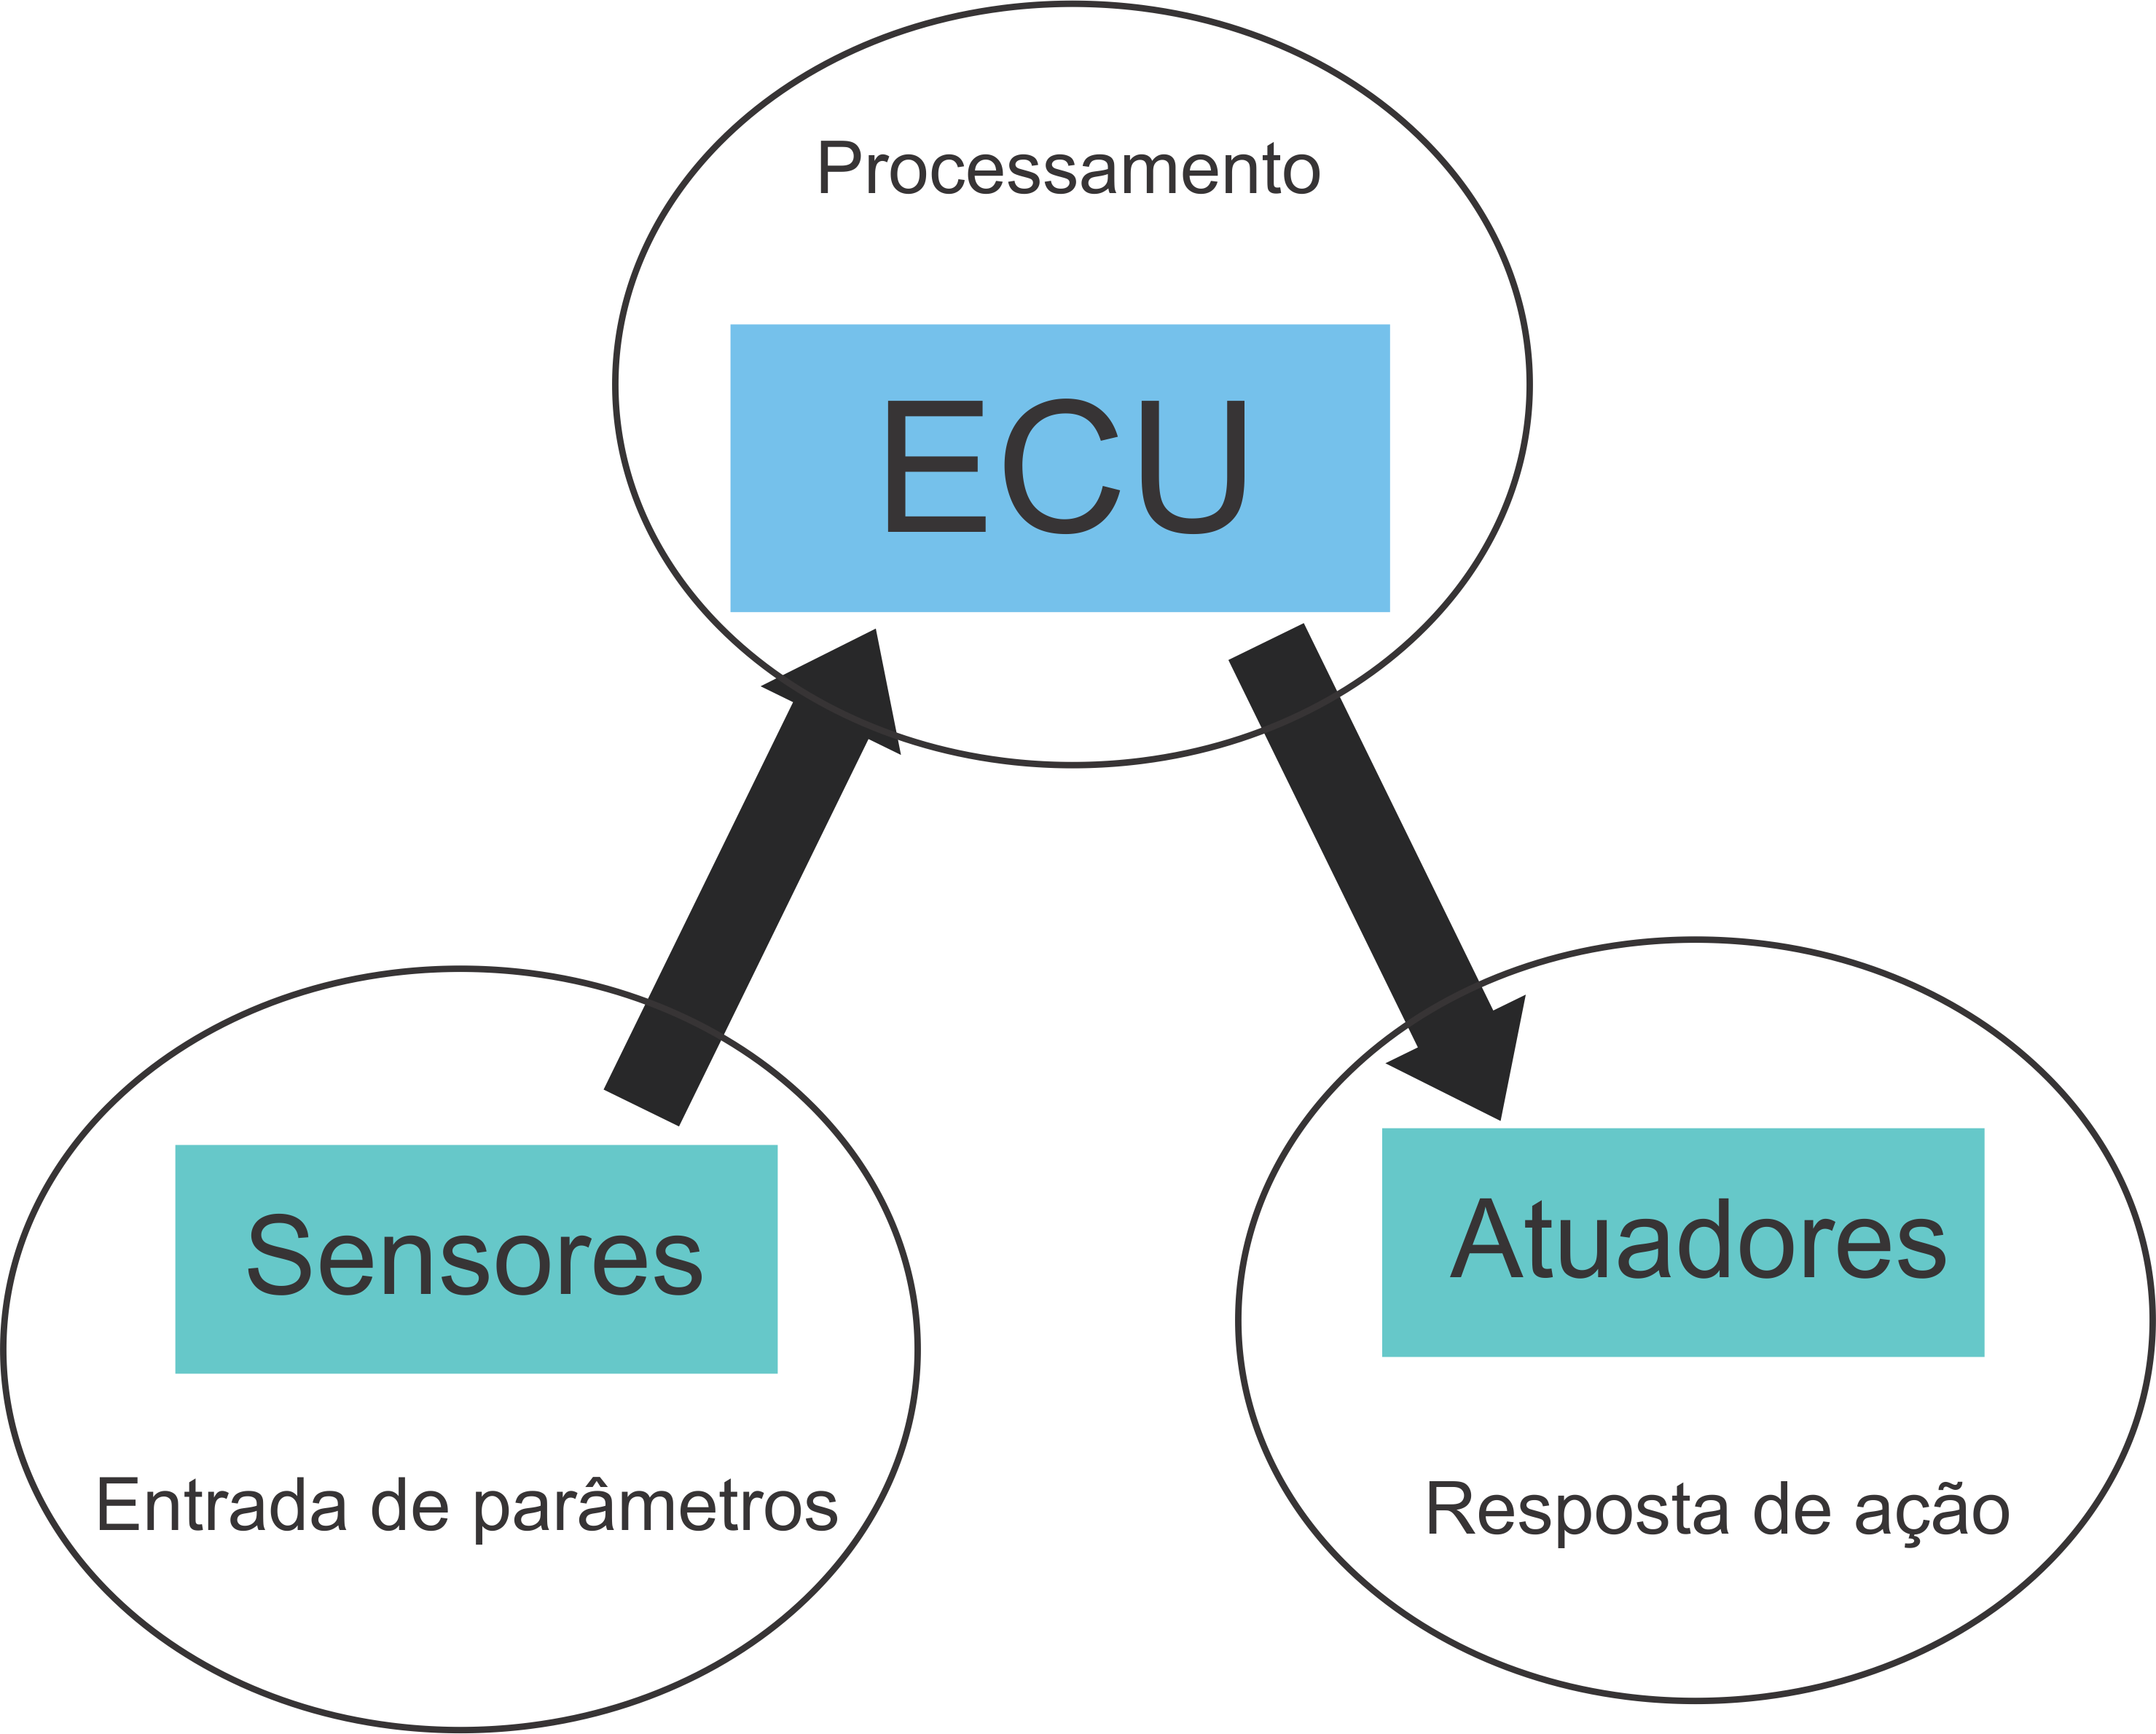
\includegraphics[scale=.34]{imagens/ecuSensorAtuador.png}}\\
\makebox[\width]{Fonte: baseado em \citeonline{navetsimonotlion}} \label{Fig:relacao_ecu_sensor_atuador}
\end{figure}

Segundo Smith, a comunicação da \textit{ECU} com os diversos componentes acontece de forma simplificada. Para esta comunicação ser simples e eficiente, os automóveis utilizam alguns protocolos para tratar da comunicação da rede interna do veículo. Estes protocolos serão explorados na sequência.

\subsection{PROTOCOLOS AUTOMOTIVOS}
Apesar dos protocolos permitirem a comunicação entre os dispositivos, \citeonline{smith} reforça que caso o veículo tenha sido fabricado antes do ano de 2000, há possibilidade de ele não possuir nenhum protocolo implementado. Para ele, os protocolos presentes nos barramentos são responsáveis por gerenciar a transmissão de pacotes de dados pela rede automotiva. Diversos sensores e dispositivos conectados nesta rede se comunicam com a finalidade de administrar o comportamento do veículo. Segundo o autor, toda a parte da comunicação crítica ocorrem nos barramentos de alta velocidade, enquanto a comunicação não crítica ocorre nos barramentos de média e baixa velocidade. Subentende-se que a comunicação crítica está relacionada a todos os controles que garantem a segurança e integridade dos ocupantes do automóvel. 

\citeonline{navetsimonotlion} afirmam que o papel central das redes está em manter os sistemas embarcados em estado de segurança, uma vez que a maioria das funções críticas estão distribuídas e necessitam da comunicação contínua entre si. Ele ainda aponta que a diversificação das redes utilizadas em todo o automóvel é justificada pela crescente necessidade da largura de banda, desempenho e outros requisitos de confiabilidade.

Cada fabricante decide qual barramento ou protocolo serão utilizados na arquitetura do veículo; entretanto, existe um protocolo comum em todos os veículos: o protocolo \textit{CAN} \cite{smith}. Em 1994, a Sociedade de Engenheiros Automotivos \textit{(Society for Automotive Engineers – SAE)}, citada por \citeonline{navetsimonotlion}, definiu uma classificação para protocolos de comunicação automotiva baseando-se na velocidade de transmissão dos dados e nas funções que seriam distribuídas pela rede (Tabela \ref{tab:tipos_redes_transmissao}). As redes de classe A possuem uma taxa de dados inferior a 10 kbps e são utilizadas para transmissão de dados de controle com tecnologias de baixo custo e estão integradas na categoria \textit{Body}. As redes classe B operam em uma velocidade de 10 a 125 kbps e se dedicam para suportar a troca de dados entre \textit{ECUs}, para reduzir o número de sensores compartilhando informações. Aplicações que precisam de comunicação em tempo real requerem redes de classe C (com velocidade de transmissão de 125 kbps a 1Mbps) ou redes de classe D (operando com velocidades superiores a 1Mbps). As redes classe C integram a comunicação das categorias \textit{Power Train} e \textit{Chassis}. Já as redes de classe D são dedicadas a dados multimídia e aplicações críticas de segurança que requeiram previsibilidade e tolerância de falhas.

\begin{table}[htb!]
\centering
\caption{Tipos de redes e suas respectivas velocidades de transmissão de acordo com a \textit{SAE}.}
\label{tab:tipos_redes_transmissao}
\begin{tabular}{cc}
\hline
Tipos de redes & \multicolumn{1}{c}{Velocidade de transmissão} \\ \hline
Classe A              & até 10 kbps                             \\
Classe B              & de 10 a 125 kbps                          \\
Classe C              & de 125 kbps a 1Mbps                       \\
Classe D              & acima de 1Mbps                            \\ \hline
\end{tabular}
\end{table}

De acordo com \citeonline{navetsimonotlion}, é comum a inclusão dos quatro tipos de redes em barramentos diferentes interligadas por \textit{gateways} na arquitetura eletrônica dos veículos atuais, conforme representado na Figura \ref{Fig:redes_gateway}. Eles ainda complementam que será possível futuramente a inclusão de um barramento dedicado aos sistemas de segurança dos ocupantes. De todos os protocolos existentes e citados pelos autores, serão explorados dois, o protocolo \textit{CAN} e o SAE J1850.

\begin{figure}[!ht]
\centering
\caption{Representação de redes distintas interligadas.} 
{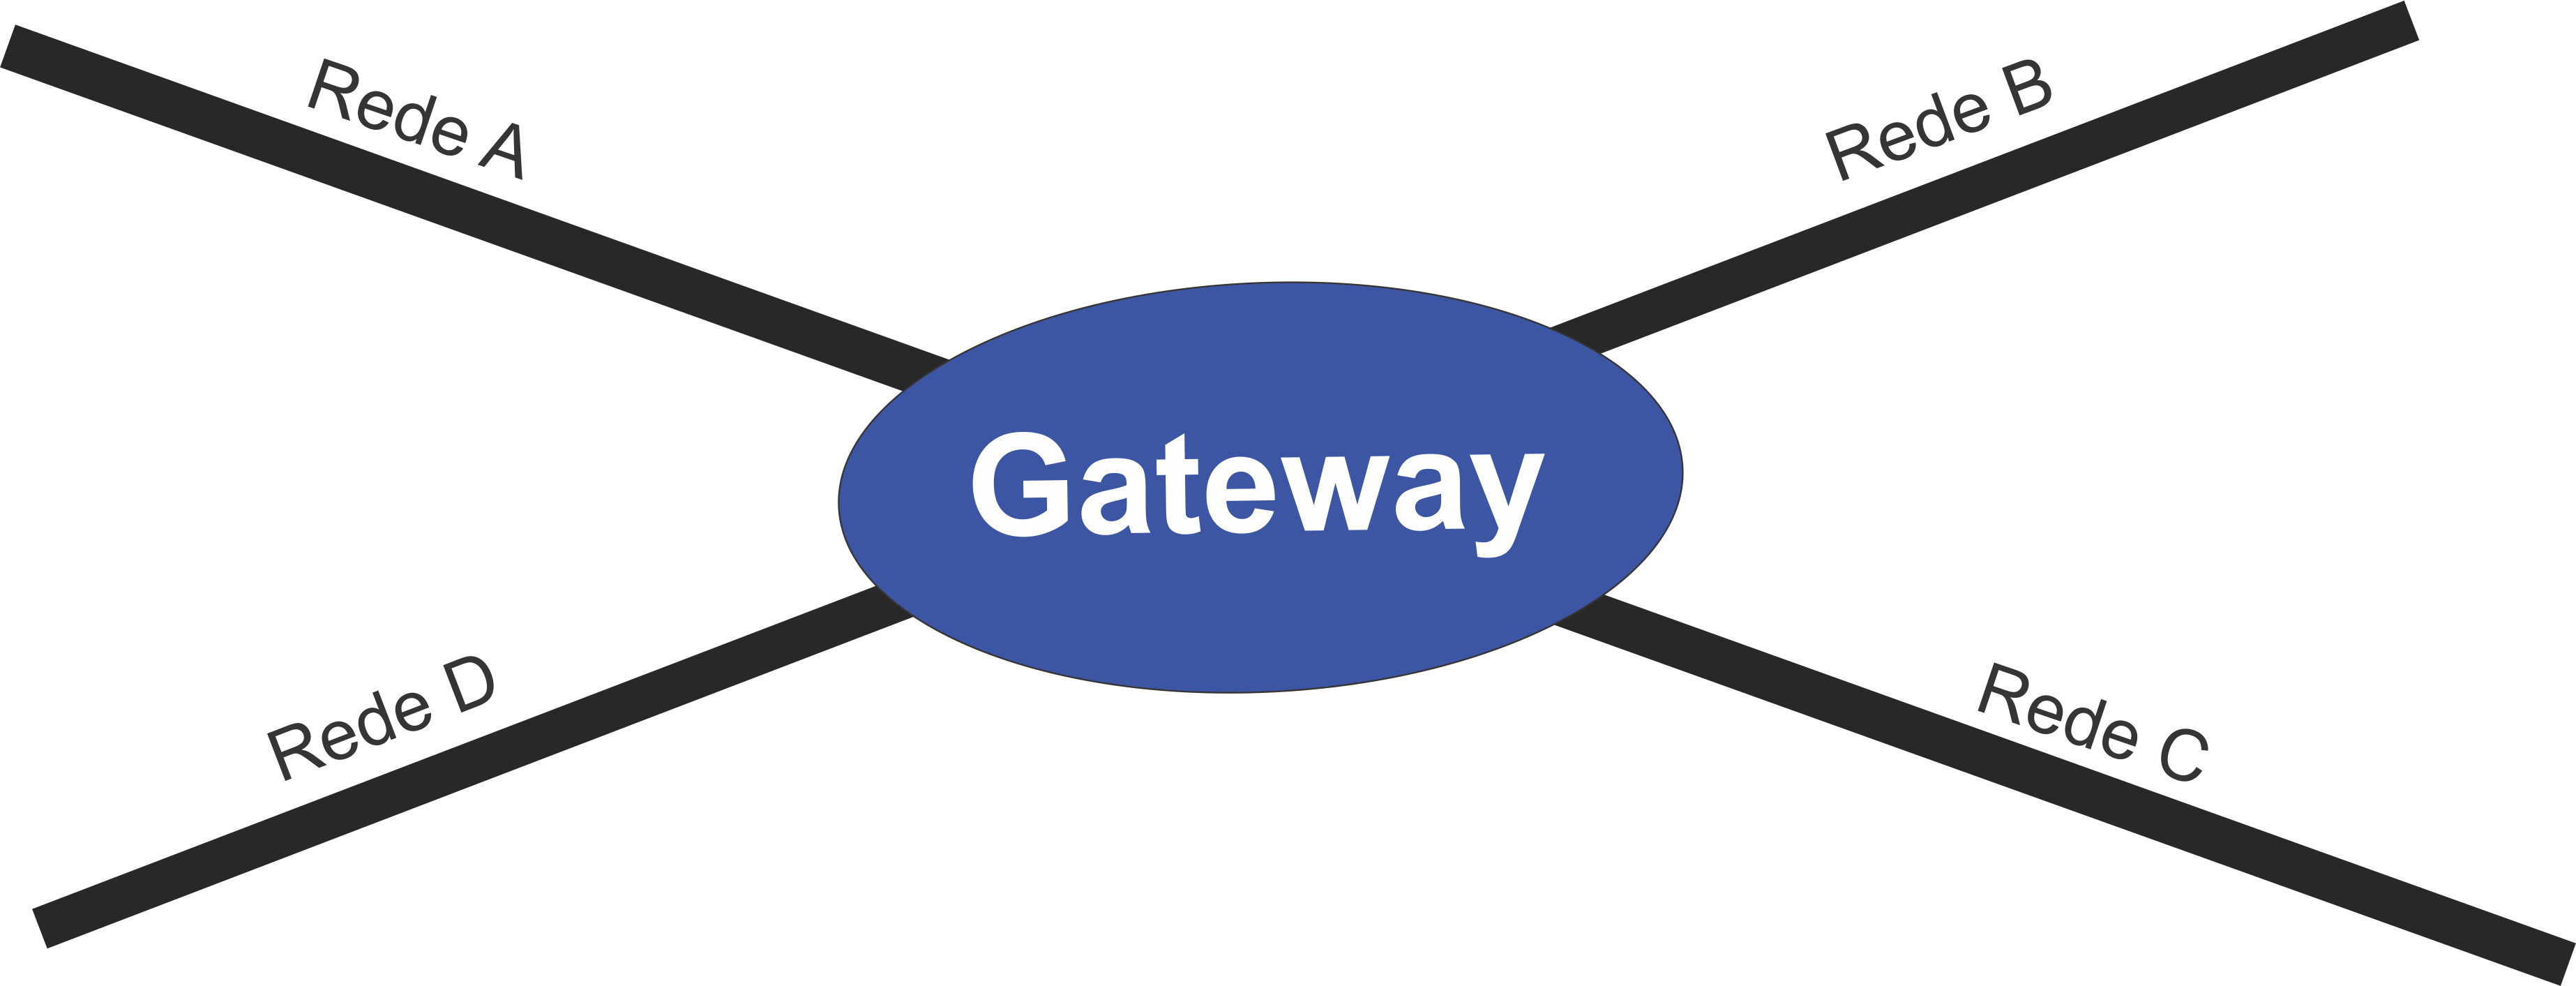
\includegraphics[scale=.35]{imagens/redesGateway.png}}\\
\makebox[\width]{Fonte: baseado em \citeonline{navetsimonotlion}} \label{Fig:redes_gateway}
\end{figure}

\subsubsection{PROTOCOLO \textit{CAN} \textit{(CONTROLLER AREA NETWORK)}}
Por volta de 1980, foi desenvolvido pela Bosch o protocolo conhecido como \textit{CAN} \textit{(Controller Area Network)}, ou simplesmente protocolo de controle de área de rede. Este protocolo foi integrado pela primeira vez em carros de produção da Mercedes na década de 90 \cite{navetsimonotlion}. \citeonline{smith} afirma que o \textit{CAN} é um protocolo simples utilizado na indústria automobilística. Este protocolo permite a comunicação de \textit{ECUs} e sistemas embarcados que estão presentes nos veículos modernos. \citeonline{navetsimonotlion} ainda complementam que as redes que utilizam esse protocolo tornaram-se as mais utilizadas nos sistemas automotivos. Por possuírem baixo custo, serem robustas e terem atrasos baixos de comunicação, o protocolo \textit{CAN} é um padrão utilizado na Europa para transmissão de dados de aplicações automotivas.

Atualmente, para controlar os sistemas da categoria \textit{Power Train} utiliza-se a \textit{CAN} como uma rede \textit{SAE} de classe C, operando de 250 a 500 kbps. Entretanto, ela também pode operar nos sistemas de categoria \textit{Body}, com uma taxa de 125 kbps. Segundo os estudos de \citeonline{smith}, o protocolo \textit{CAN} possui dois tipos de pacotes que são chamados de \textit{standard} (padrão) e \textit{extended} (extendido).

Os pacotes \textit{standard} possuem quatro elementos, que são o ID de arbitragem, extensão de ID, código do tamanho dos dados e os própios dados. Quando um dispositivo tenta se comunicar é enviado ID de arbitragem, que é uma mensagem de broadcast que identifica o ID deste dispositivo. Quando dois pacotes são transmitidos ao mesmo tempo no barramento, aquele com ID de arbitragem menor vence. \citeonline{navetsimonotlion} apontam esta técnica como sendo um método utilizado por este protocolo para evitar colisões ao acessar o barramento. Voltando aos estudos de \citeonline{smith}, ele afirma que o bit que define a extensão de ID tem o valor 0 para pacotes \textit{standard}. O código do tamanho dos dados define o tamanho dos dados, que pode variar de 0 a 8 bytes. O tamanho máximo dos dados transportados por este pacote pode ter no máximo 8 bytes.

Já os pacotes \textit{extended}, segundo o autor, são semelhantes ao \textit{standard}, com exceção de possuir espaço maior para armazenar IDs mais longos. Estes pacotes foram desenvolvidos para caberem dentro do formato \textit{standard} para manter a compatibilidade com as versões anteriores. Desta forma, caso algum sensor tenha suporte somente para pacotes \textit{standard}, ele não será invalidado caso sejam transmitidos pacotes \textit{extended} na mesma rede. Dentre outras particularidades deste pacote, \citeonline{smith} ainda reforça que existem outros protocolos adicionais específicos de alguns fabricantes (protocolo ISO-TP, \textit{CANopen}, GMLAN) que seguem o padrão \textit{CAN}, da mesma forma que o pacote \textit{CAN} \textit{extended} (Figura \ref{Fig:implementacoes_can}).

\begin{figure}[!ht]
\centering
\caption{Representação de outros protocolos implementados no padrão \textit{CAN}.} 
{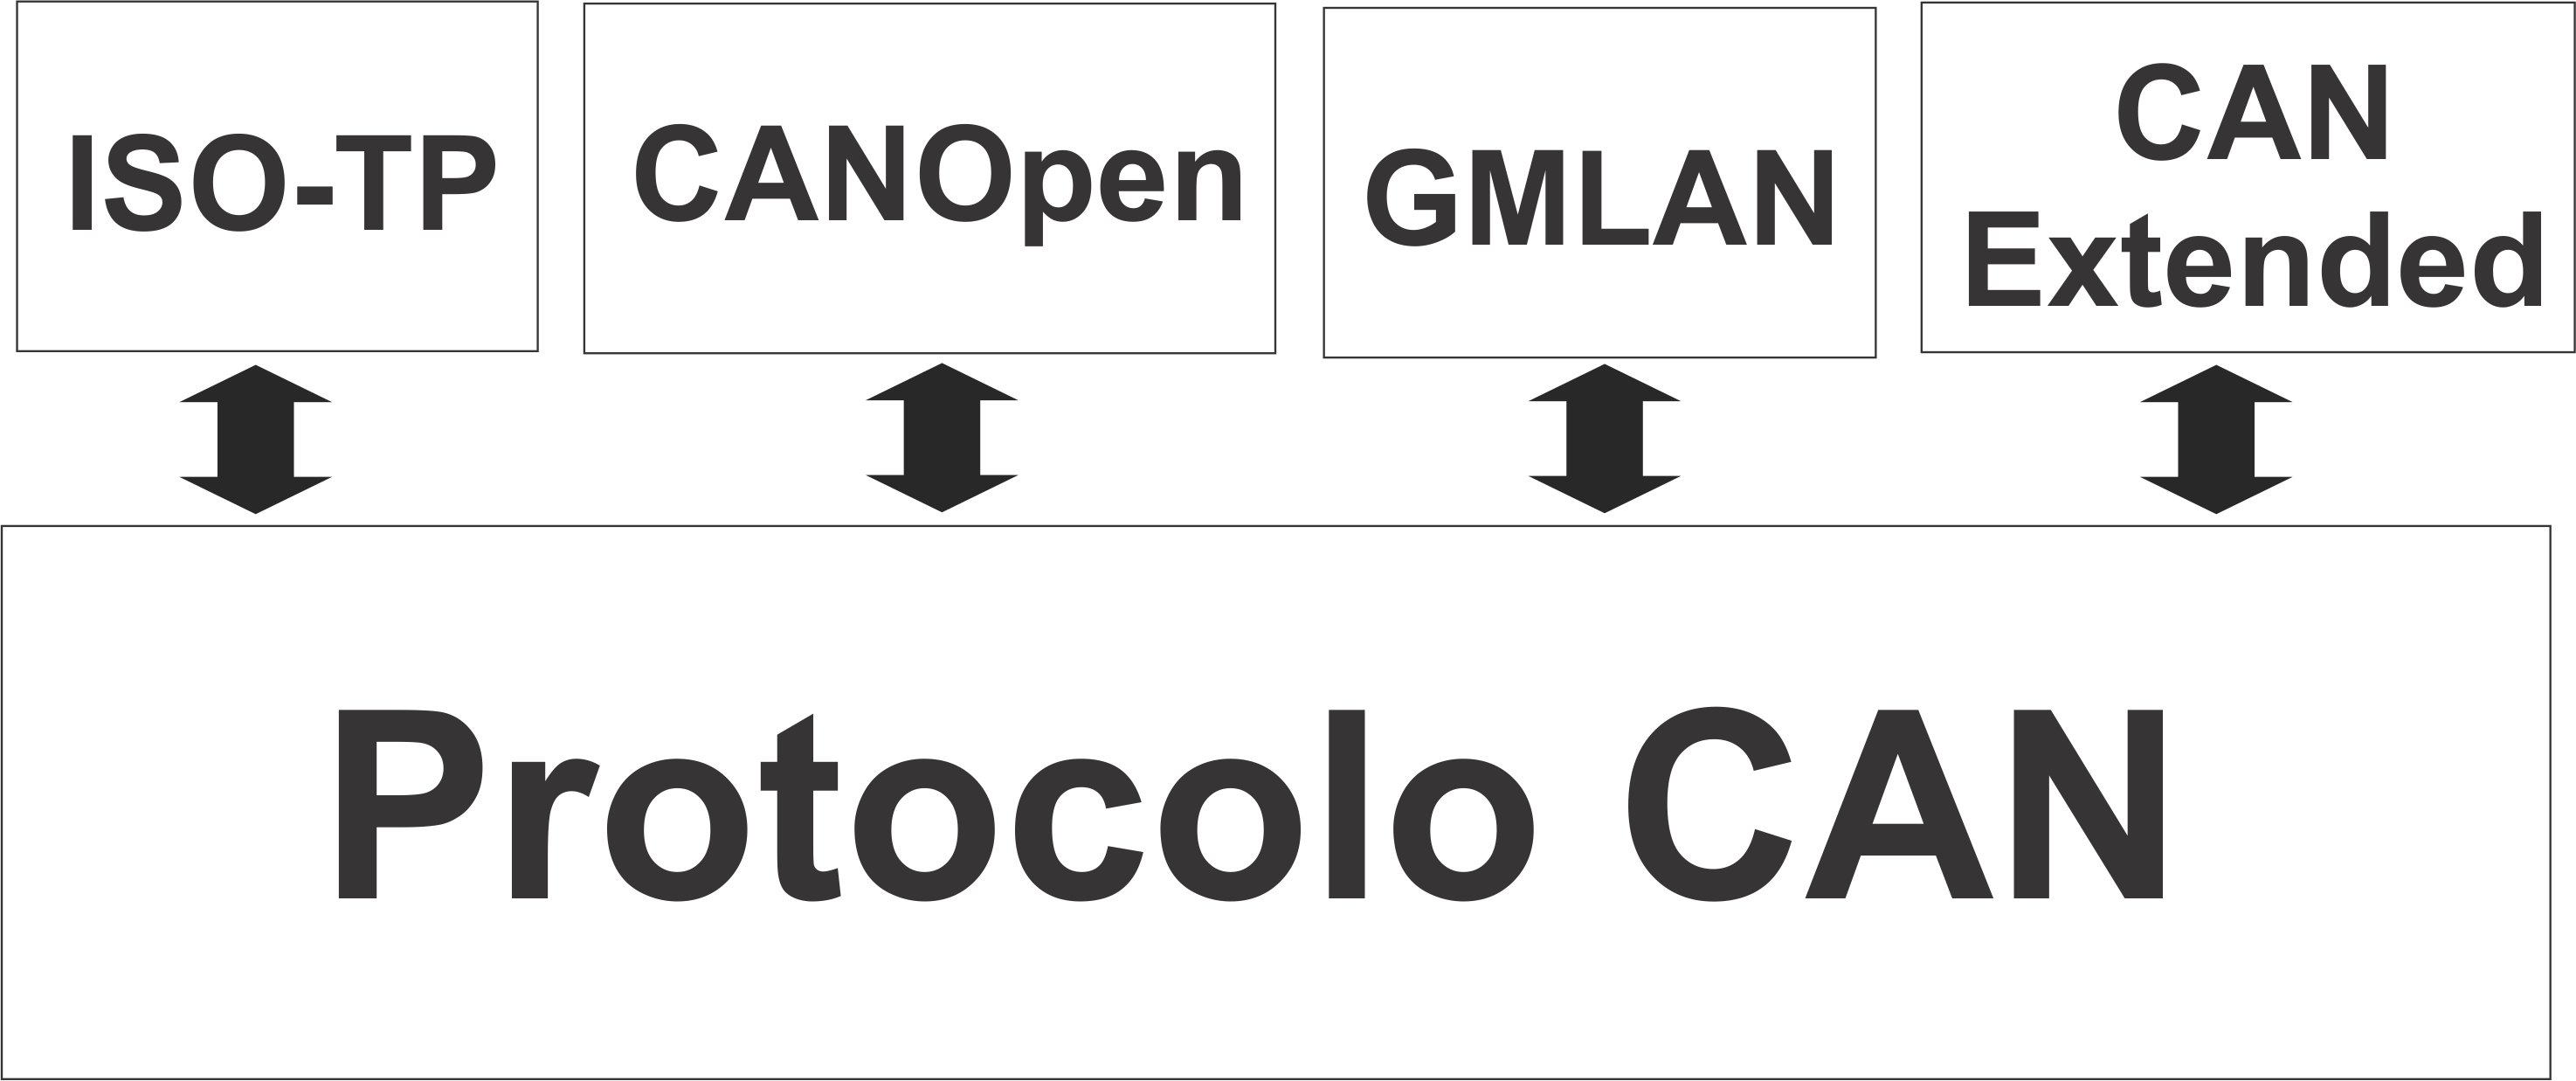
\includegraphics[scale=.25]{imagens/protocoloCanEVariacoes.png}}\\
\makebox[\width]{Fonte: baseado em \citeonline{smith}} \label{Fig:implementacoes_can}
\end{figure}

Segundo \citeonline{navetsimonotlion}, o protocolo \textit{CAN} define apenas a camada física e a camada de link dos dados. Para tratar a padronização de inicialização, implementar a segmentação de dados ou enviar mensagens periódicas, foram propostos diversos protocolos de nível superior.

\subsubsection{PROTOCOLO SAE J1850}
O protocolo SAE J1850 foi implementado originalmente por volta de 1994, segundo \citeonline{smith}, e ainda pode ser encontrado nos veículos atuais. Comparado com o protocolo \textit{CAN}, este é mais lento, entretanto, seu custo de implantação é mais barato. \citeonline{navetsimonotlion} menciona que são definidas duas variações para este protocolo. \citeonline{smith} as define como modulação de largura de pulso \textit{(pulse width modulation – PWM)} e largura de pulso variável \textit{(variable pulse width – VPW)}, conforme representado pela Figura \ref{Fig:implementacoes_saej1850}. O \textit{PWM} trabalha com uma velocidade de 41.6 Kbps, enquanto o \textit{VPW} trabalha com 10.4 Kbps.

\begin{figure}[!ht]
\centering
\caption{Variações do protocolo SAE J1850.} 
{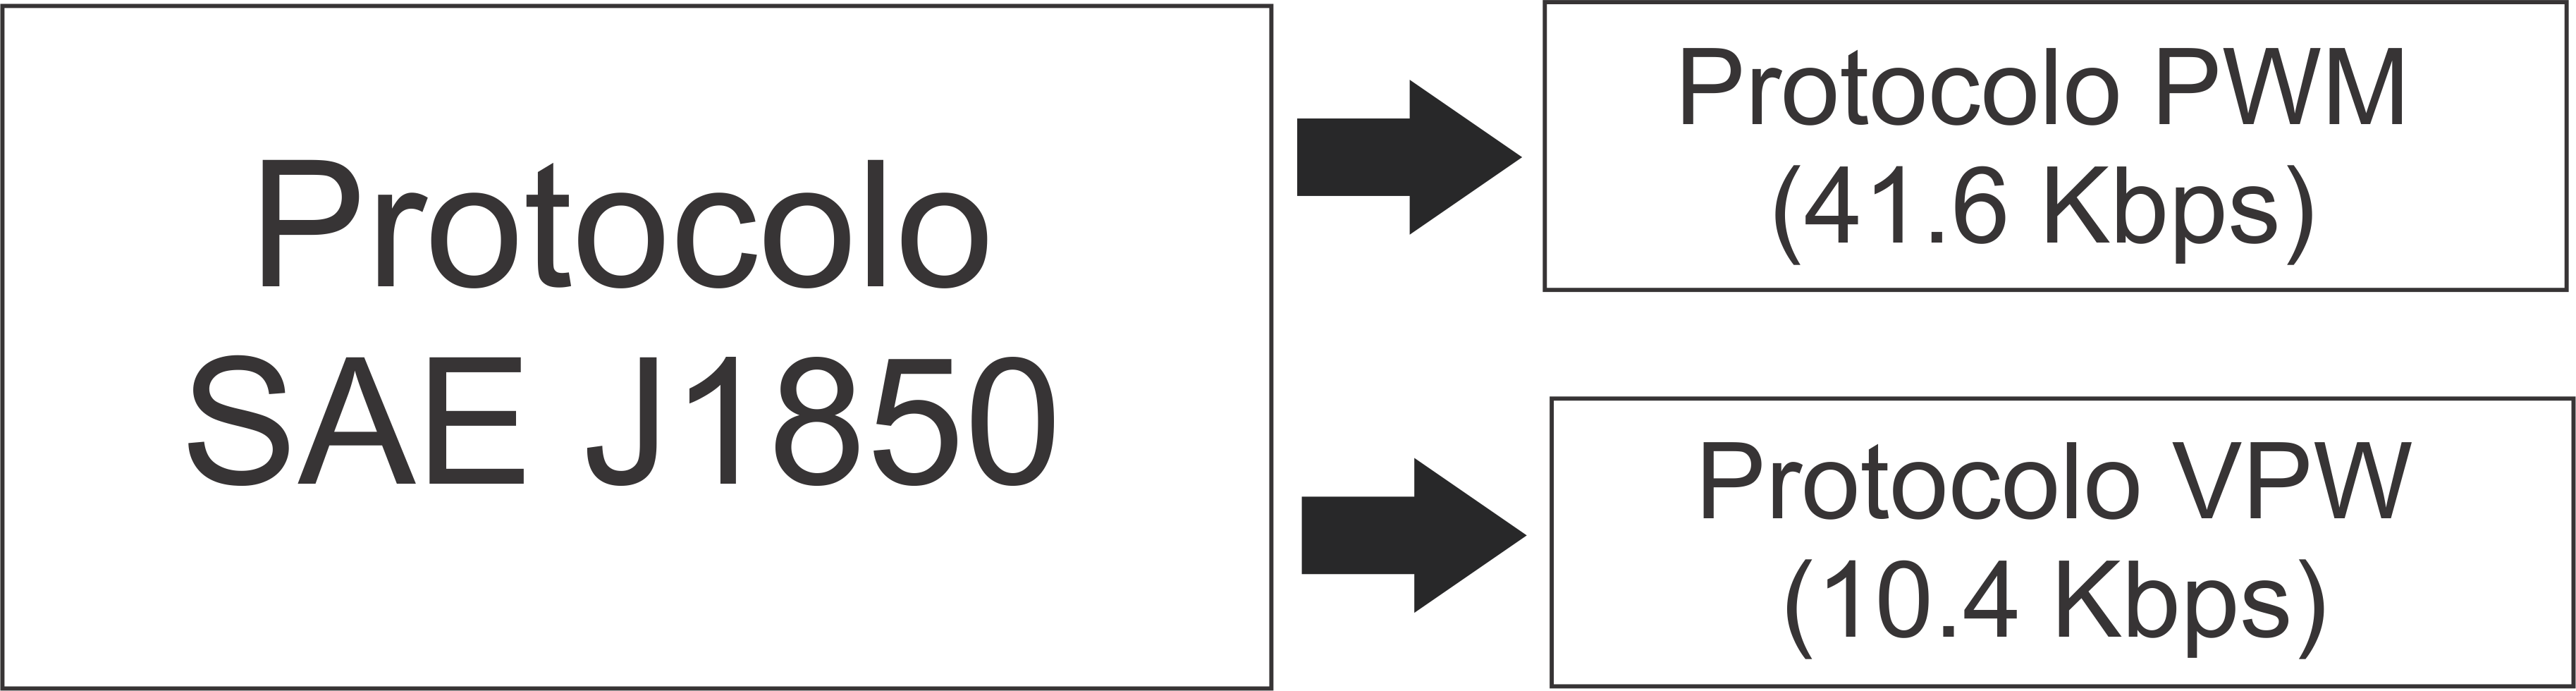
\includegraphics[scale=.25]{imagens/protocoloSaeJ1850.png}}\\
\makebox[\width]{Fonte: baseado em \citeonline{smith, navetsimonotlion}} \label{Fig:implementacoes_saej1850}
\end{figure}

\citeonline{navetsimonotlion} afirmam que para tratar dos controles dos sistemas da categoria \textit{Body} ou de diagnósticos, os Estados Unidos adotaram este protocolo SAE J1850 de classe B pois as comunicações não possuíam requisitos de transmissão em tempo real.

Analisando os protocolos apresentados, observa-se que para determinada aplicação é utilizado um protocolo específico.  E cada protocolo tem uma classificação quanto à sua velocidade de transmissão pelo \textit{SAE}. Existem outros protocolos que estão presentes na rede automotiva, como o \textit{Keyword Protocol} e ISO 9141-2, explorados por \citeonline{smith}, os protocolos IDB-1394, \textit{VAN (Vehicle Area Network)} e \textit{TTCAN}, explorados por \citeonline{navetsimonotlion}, ou ainda os protocolos \textit{LIN (Local Interconnect Protocol)}, \textit{MOST (Media Oriented Systems Transport)} e o \textit{FlexRay}, todos explorados na literatura de ambos.

Observando-se o comportamento da rede automotiva, nota-se a presença de vários protocolos responsáveis pela comunicação de diversos dispositivos que são destinados a realizar uma determinada função específica no veículo. Entretanto, também existe a necessidade de monitorar essa rede para realizar eventuais diagnósticos neste sistema, e o nome dado para esta função se chama diagnóstico de bordo \textit{(OnBoard Diagnostics – OBD)} \cite{navetsimonotlion}.

\subsection{CONECTOR \textit{OBD-II (ONBOARD DIAGNOSTICS)}}\label{subsecaoobd}
Também conhecido como conector de diagnóstico de conexão \textit{(Diagnostic Link Connector – DLC)}, o conector \textit{OBD-II} está integrado em grande parte dos veículos, e permite a comunicação com a rede interna automotiva conforme exemplificado por \citeonline{smith}. De acordo com \citeonline{navetsimonotlion}, a introdução de sistemas informáticos capazes de memorizar grandes quantidades de informação de um automóvel possibilitou o diagnóstico de bordo, que se refere ao autodiagnóstico e a facilidade de emissão de relatórios. Para \citeonline{smith}, o conector \textit{OBD-II} é utilizado principalmente pela mecânica para analisar e solucionar eventuais problemas com o automóvel. A Figura \ref{Fig:obd2} mostra a localização do conector \textit{OBD-II} em um automóvel.

\begin{figure}[!ht]
\centering
\caption{Foto do conector \textit{OBD-II}.} 
{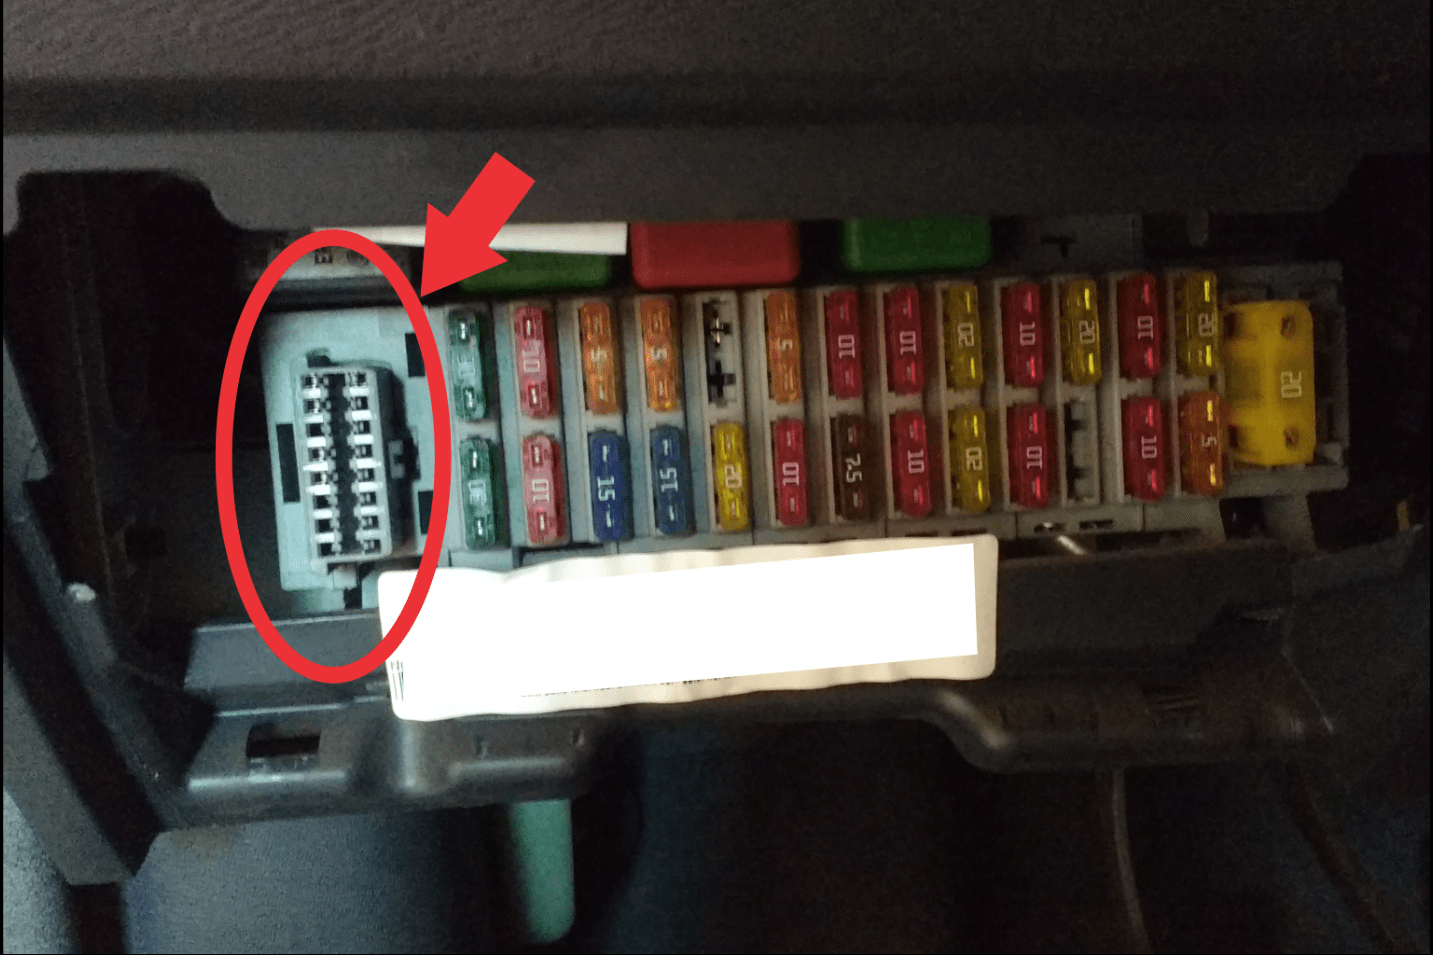
\includegraphics[scale=.19]{imagens/obdII.png}}\\
\makebox[\width]{Fonte: foto tirada pelo autor} \label{Fig:obd2}
\end{figure}

Ao apresenta uma falha, o sistema guarda informações relacionadas a ela e aciona uma luz de aviso do motor no painel do motorista, conhecida como luz indicadora de mau funcionamento (\textit{malfunction indicator lamp – MIL}, Figura \ref{Fig:luz_mil}). Embora o diagnóstico tenha se limitado a essa luz indicadora, conforme \citeonline{navetsimonotlion} apresentam, a comunicação dos sistemas \textit{OBD} recentes são padronizados, como por exemplo a padronização de dados monitorados, codificação padronizada e relatórios de uma lista de falhas específicas, conhecidas como códigos de diagnósticos de problemas \textit{(Diagnostic Trouble Codes – DTC)}. De acordo com \citeonline{smith}, as verificações de rotina são tratadas pela \textit{ECU} primária do veículo, o qual ele se refere de módulo de controle do \textit{powertrain} \textit{(PCM)}. Para controlar a emissão de gases de escape ao longo da vida útil de um veículo, segundo \citeonline{navetsimonotlion}, foi necessário uma padronização na especificação \textit{OBD-II}, que passou a ser obrigatória para todos os carros comercializados nos Estados Unidos a partir de 1996. Este padrão definia com precisão diversos aspectos relacionados ao diagnóstico, avaliação e monitoramento do veículo.

\begin{figure}[!ht]
\centering
\caption{Foto da luz \textit{MIL} do painel.} 
{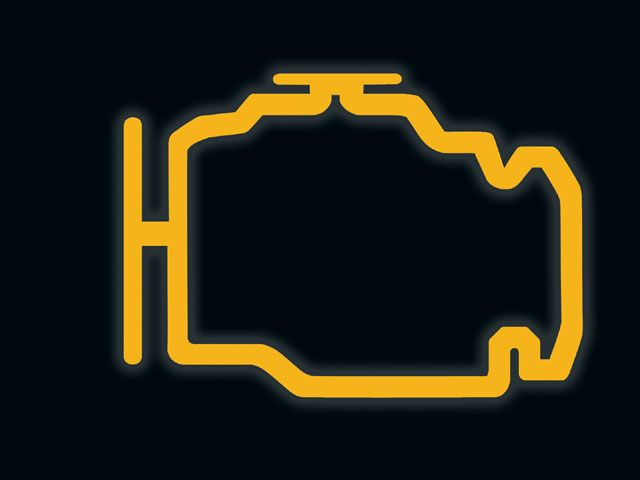
\includegraphics[scale=.15]{imagens/luzMil.jpg}}\\
\makebox[\width]{Fonte: imagem extraída do site https://goo.gl/CiSaec} \label{Fig:luz_mil}
\end{figure}

Voltando à parte de diagnósticos, com base nos estudos de \citeonline{smith}, todos os códigos de falha, como os \textit{DTCs} são armazenados no \textit{PCM}. Ele ainda complementa dizendo que os \textit{DTCs} são armazenados em locais diferentes. Enquanto os \textit{DTCs} baseados em memória ficam armazenadas na memória RAM e apagados quando a energia da bateria acaba, os \textit{DTCs} mais sérios que estão relacionados com falhas permanentes ficam armazenados em locais onde a persistência de dados é maior e consequentemente sobreviverão à uma queda de energia.

A Figura \ref{Fig:rede_veicular} representa de maneira simplificada como ocorre a comunicação entre os dispositivos na rede interna automotiva.

\begin{figure}[!ht]
\centering
\caption{Diagrama representando a arquitetura da rede veicular.} 
{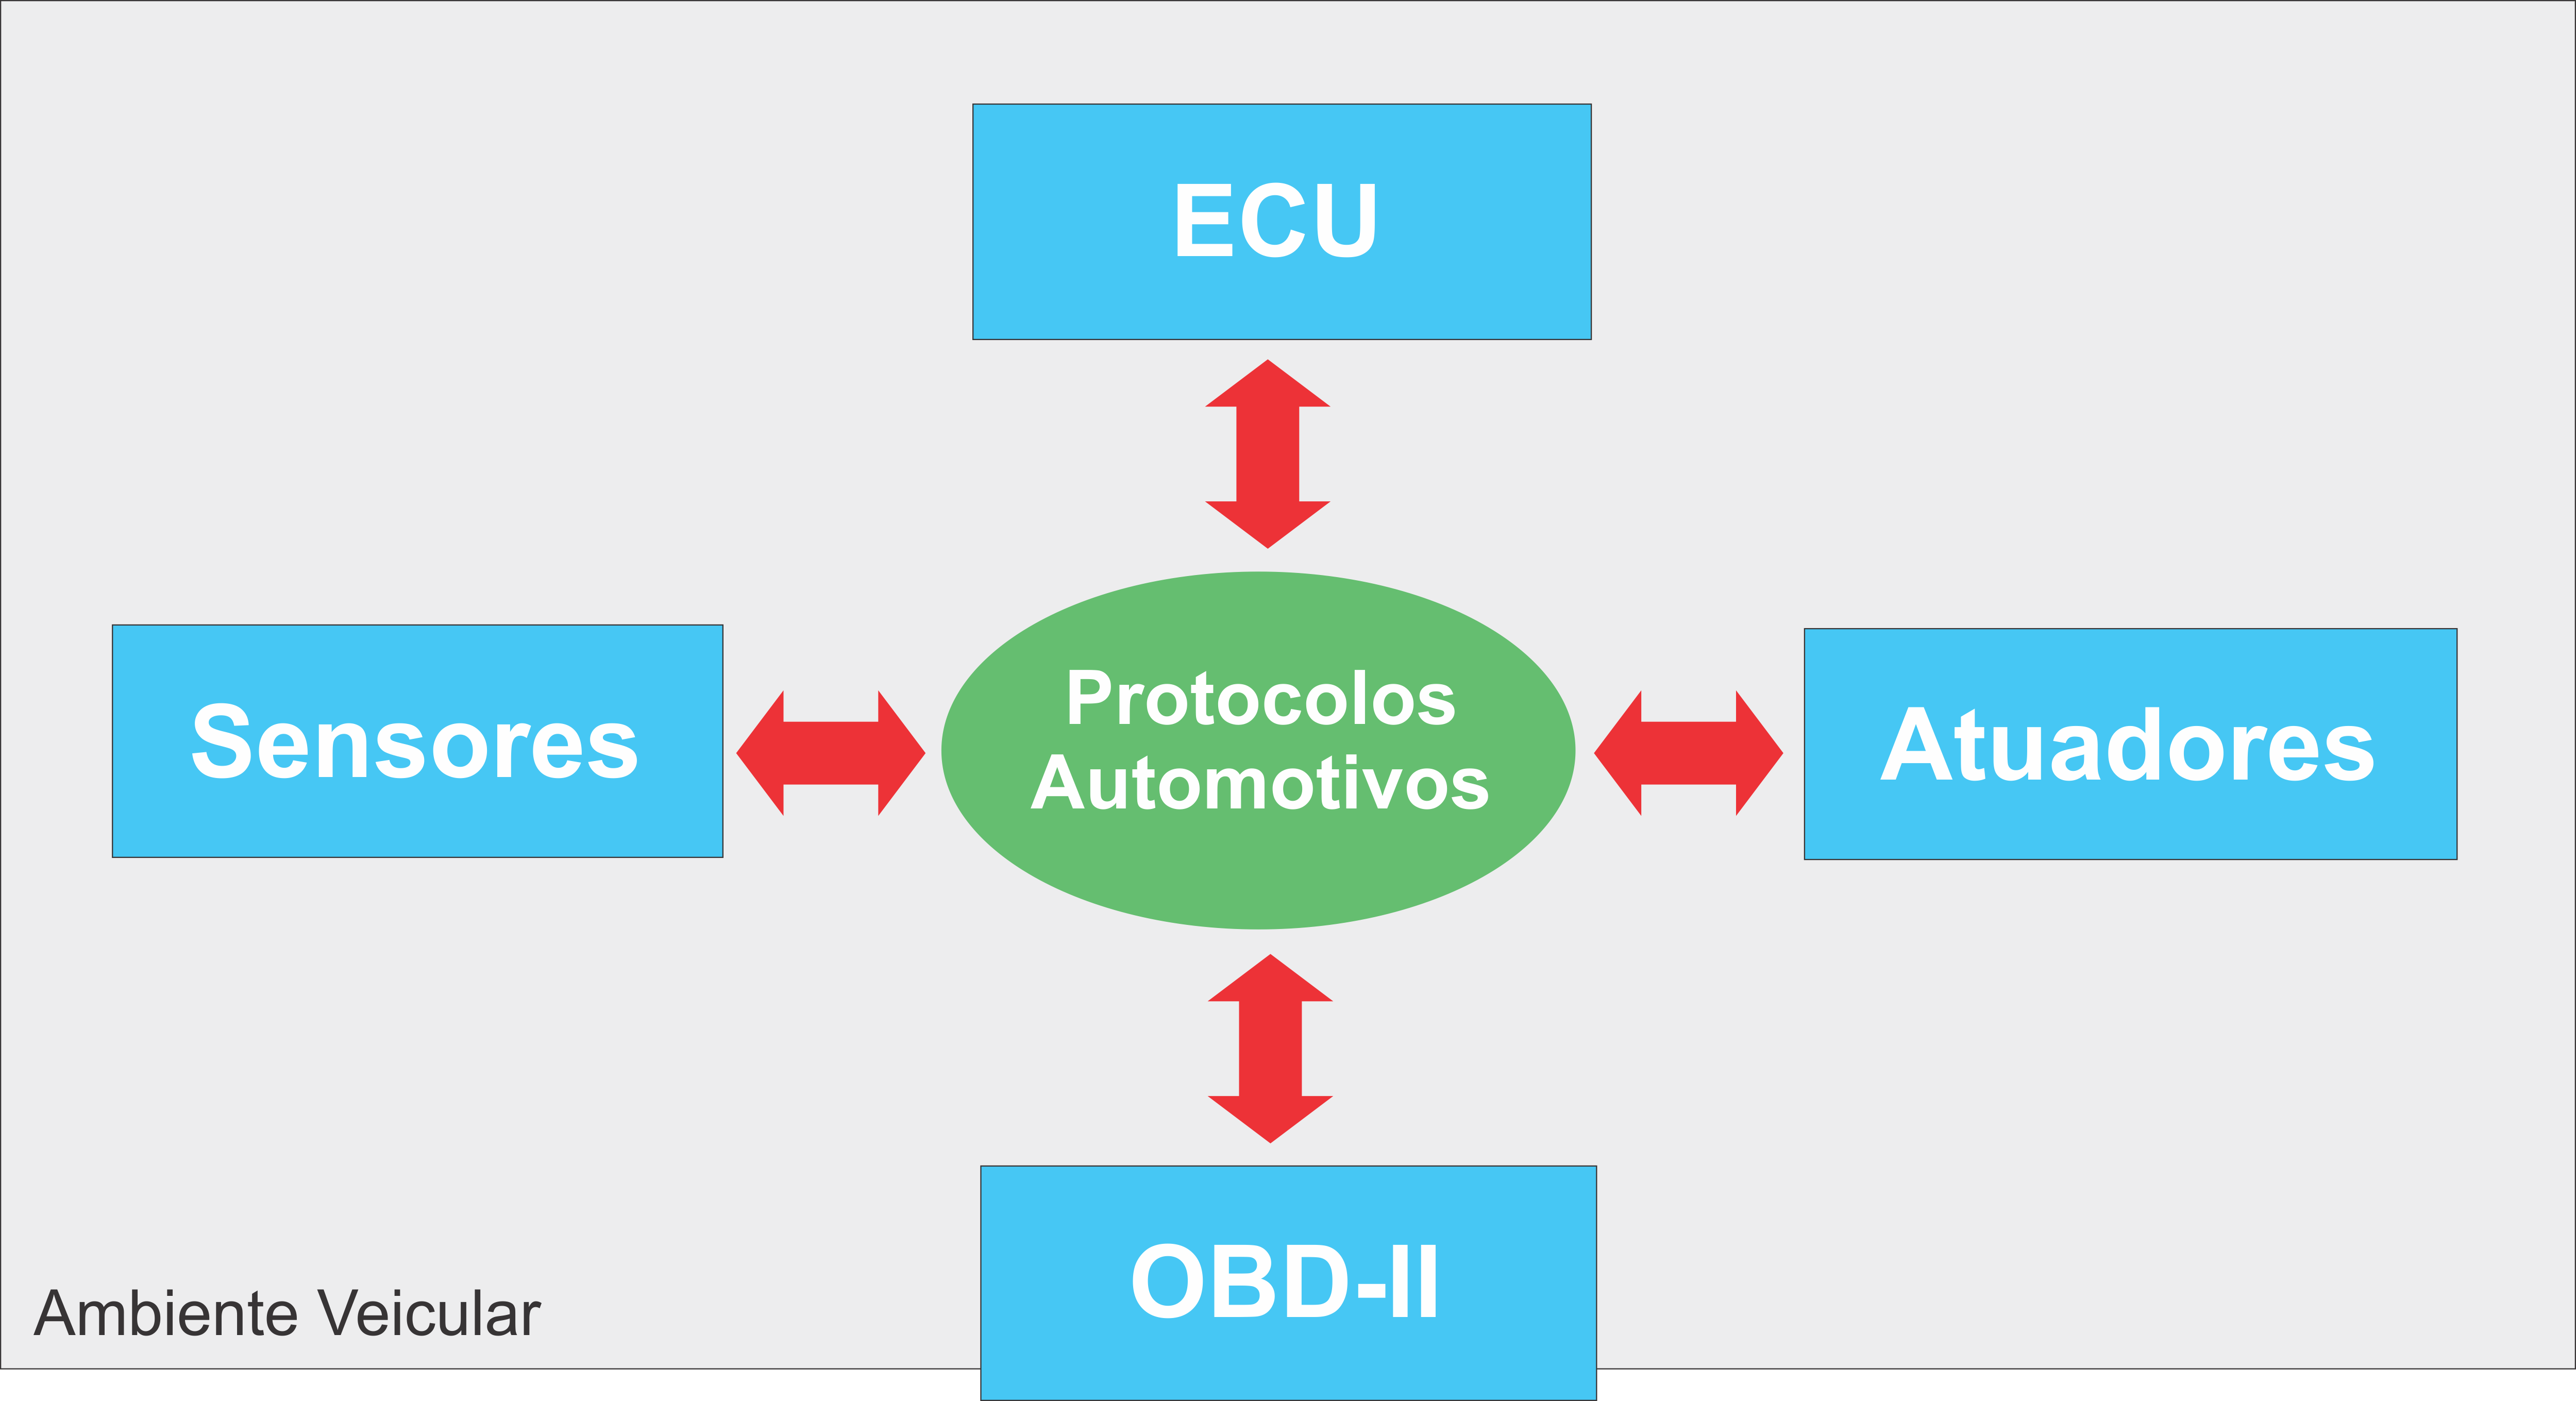
\includegraphics[scale=.32]{imagens/arquiteturaRedeVeicular.png}}\\
\makebox[\width]{Fonte: baseado em \citeonline{navetsimonotlion} e \citeonline{smith}} \label{Fig:rede_veicular}
\end{figure}

\section{ELM327}
A lei atualmente obriga, segundo a \citeonline{elmeletronics}, que todos os automóveis produzidos forneçam uma interface para a conexão de dispositivos de teste e diagnóstico. Esta interface apresentada na subseção \ref{subsecaoobd} como \textit{OBD-II}, segue as mesmas especificações dos protocolos da rede interna automotiva, o que permite a interação com ela somente se utilizar os mesmos padrões que foram estabelecidos por esta rede. Entretanto, a \citeonline{elmeletronics} ressalta que tais padrões não são compatíveis com computadores ou outros dispositivos inteligíveis, como um smartphone, por exemplo. Para solucionar este problema e permitir a compatibilidade, o ELM327 foi desenvolvido para servir de intermediário entre a porta \textit{OBD-II} - presente nos automóveis - com a interface serial padrão (RS232) presente nos computadores. A \citeonline{elmeletronics} ainda afirma que este dispositivo é capaz de identificar e interpretar nove protocolos automotivos mais o padrão J1939 utilizado por ônibus e caminhões. Desta maneira, com o ELM327 é possível utilizar um computador para se comunicar com a rede interna de um automóvel.

O ELM327 se conecta ao computador por meio da interface serial, que segundo a \citeonline{elmeletronics}, esta interface pode ser virtualizada com adaptadores USB, ou por meio de dispositivos com suporte \textit{bluetooth}. O fabricante reforça que o meio que o dispositivo usa para se conectar ao computador não tem muita relevância, pois para se comunicar com o veículo através da rede, basta apenas uma aplicação que faça o envio ou recebimento dos dados. Entretanto, para garantir a comunicação, alguns ajustes devem ser configurados, como a configuração da porta e a taxa de dados correta, conforme abordados no manual. A Figura \ref{Fig:elm327} mostra como é um dispositivo ELM327 \textit{Bluetooth}, e a Figura \ref{Fig:rede_veicular_elm327} expressa como este dispositivo se integra com o automóvel.

\begin{figure}[!ht]
\centering
\caption{Foto do ELM327 \textit{Bluetooth}.} 
{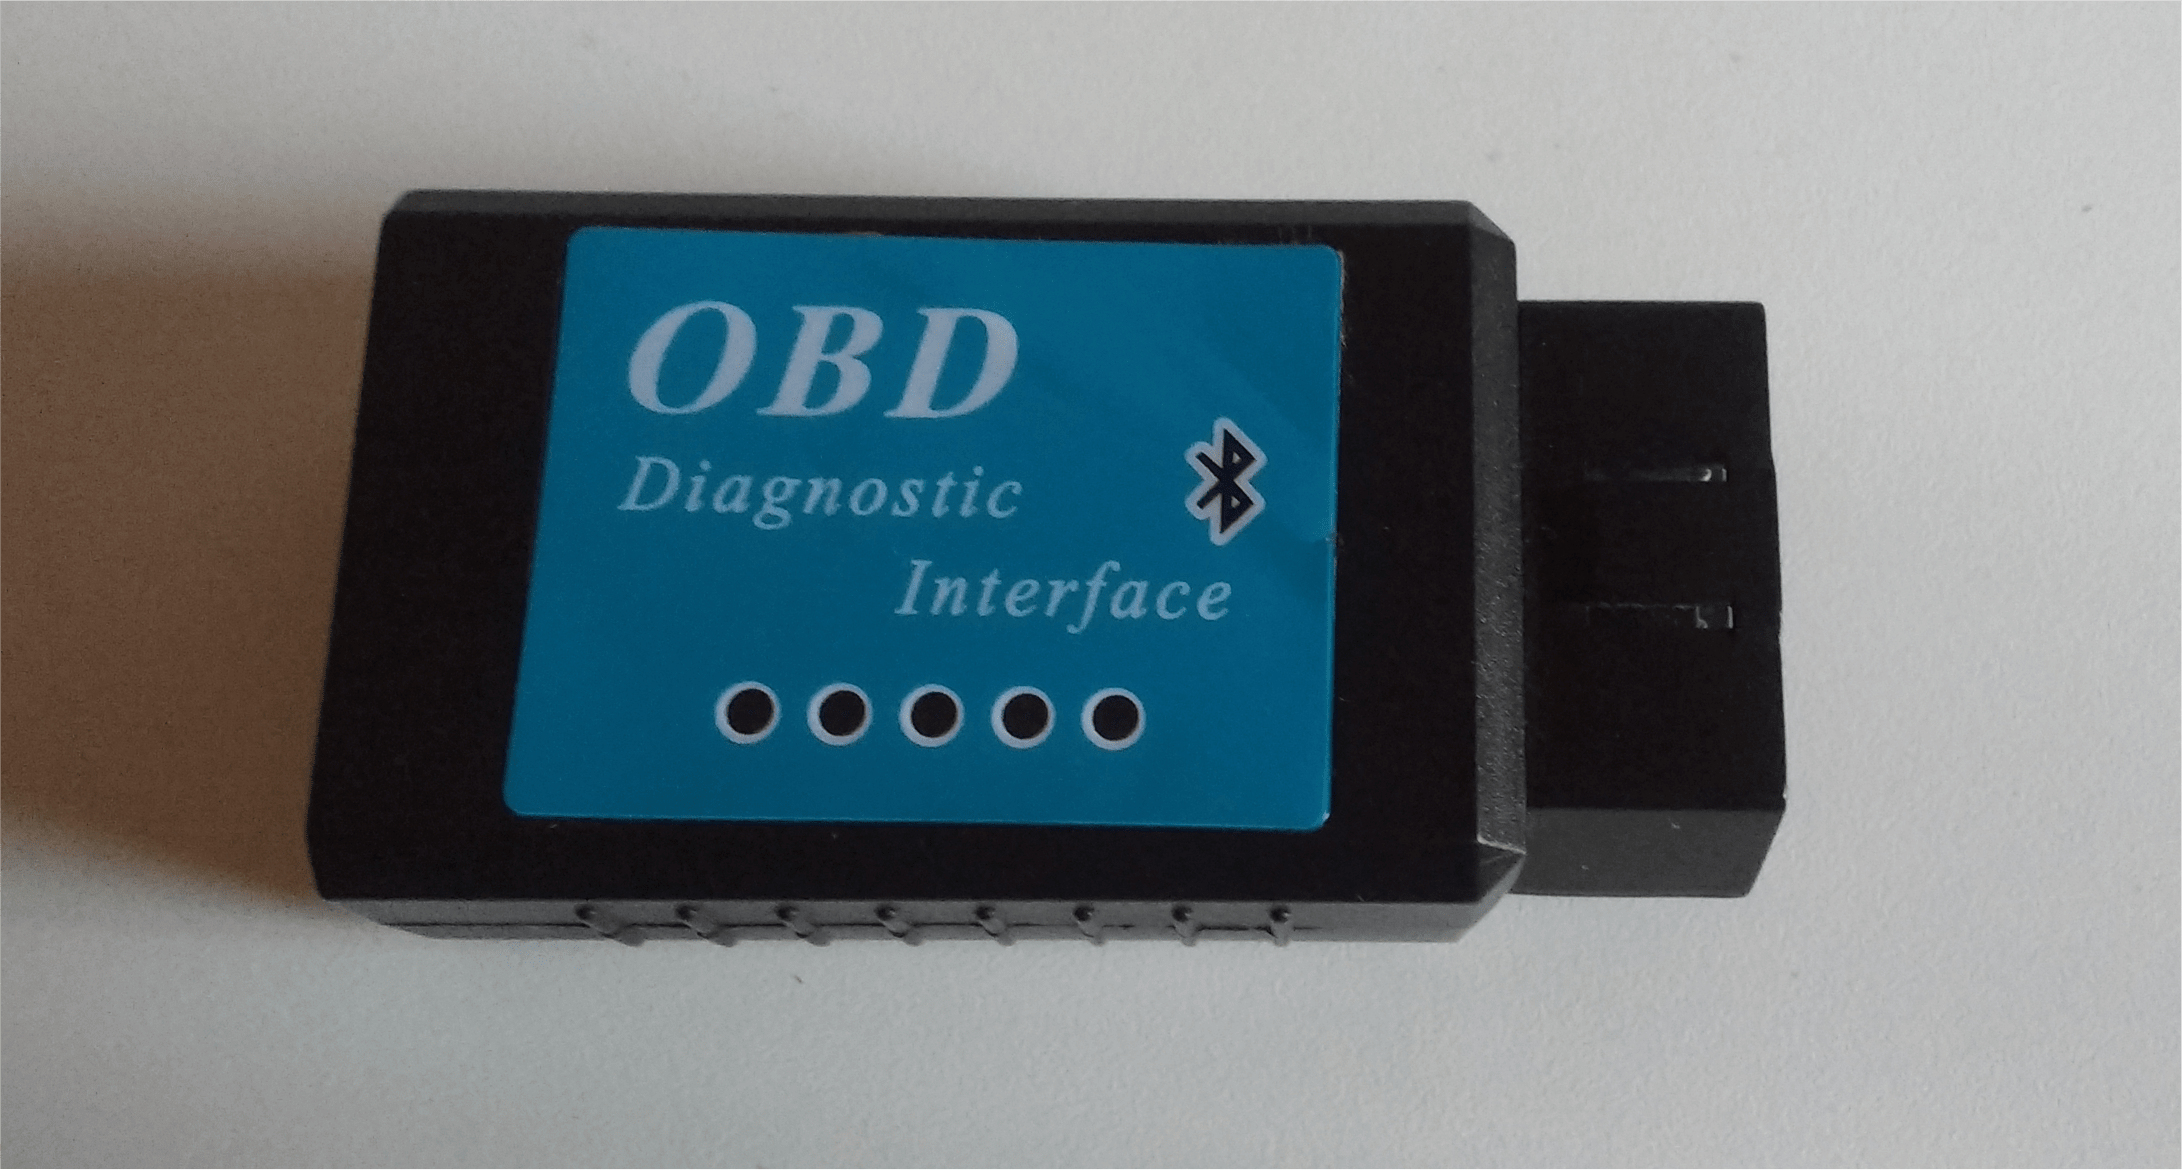
\includegraphics[scale=.16]{imagens/elm327-min.png}}\\
\makebox[\width]{Fonte: foto tirada pelo autor} \label{Fig:elm327}
\end{figure}

\begin{figure}[!ht]
\centering
\caption{Diagrama representando a interação do ELM327 com a rede automotiva.} 
{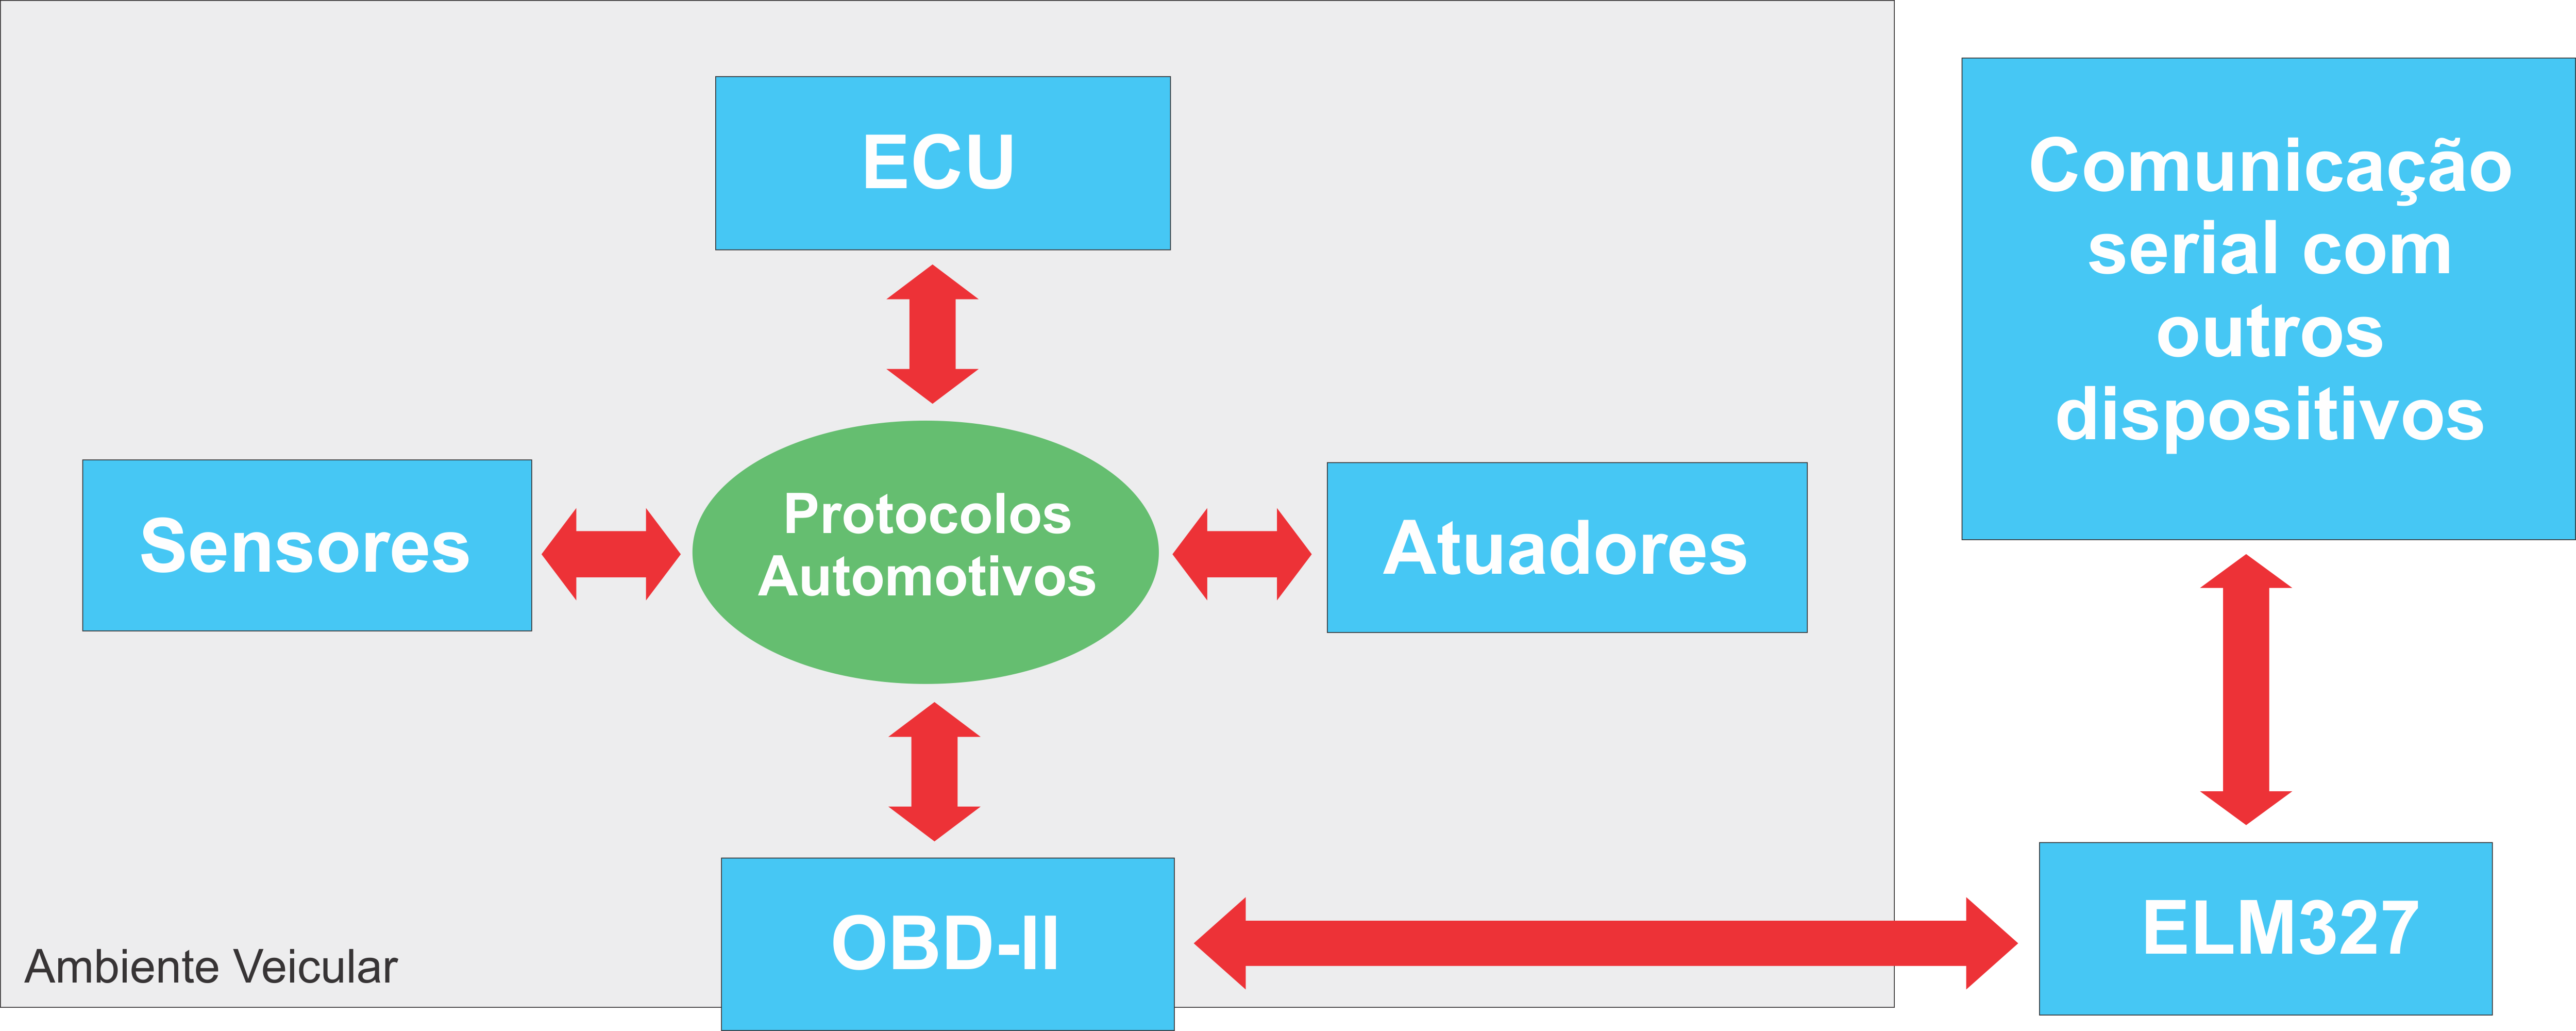
\includegraphics[scale=.35]{imagens/arquiteturaRedeVeicularELM327.png}}\\
\makebox[\width]{Fonte: baseado em \citeonline{elmeletronics}} \label{Fig:rede_veicular_elm327}
\end{figure}

Existem dois tipos de comandos que podem ser enviados. Os comandos que se destinam ao próprio dispositivo, e os comandos destinados ao veículo. Segundo a \citeonline{elmeletronics}, os comandos destinados ao dispositivo começam com os caracteres ‘AT’, enquanto os destinados à rede veicular contêm dígitos hexadecimais. Ele ainda ressalta que o ELM327 apenas converte os protocolos, não realizando nenhum tipo de validação dos dados transmitidos. Entretanto, este dispositivo garante a entrega dos dados nas extremidades, ou seja, garante que os dados sejam transmitidos tanto para o computador quanto para o veículo.

\subsection{COMANDOS AT}
Como visto anteriormente, os comandos ‘AT’ são destinados ao próprio dispositivo ELM327. Existem vários parâmetros dentro dele que podem ser ajustados para modificar seu comportamento, segundo o fabricante. Esses comandos são semelhantes aos utilizados pelos modems para a configuração interna \cite{elmeletronics}.

\subsection{COMANDOS \textit{OBD}}
Quando um comando é enviado sem as iniciais ‘AT’, é entendido como comando \textit{OBD} para o veículo. Desta forma, o dispositivo apenas verifica se o comando enviado é um algarismo hexadecimal ou uma sequencia aleatória de caracteres, e logo após transmite o dado ao veículo. Para a \citeonline{elmeletronics}, estes dados são empacotados e enviados ao automóvel. Os comandos enviados ao veículo necessitam geralmente de mais quatro bytes adicionais: três bytes de cabeçalho e um byte de verificação de erro, que devem ser incluídos junto aos dados que serão enviados. Contudo, o ELM327 adiciona estes bytes extras ao comando, abstraindo esta necessidade do usuário.

O comprimento dos comandos \textit{OBD} pode variar de um a sete bytes, sendo este último o limite máximo aceito pelo dispositivo. Ao empacotar e enviar o comando pela interface \textit{OBD}, o dispositivo fica monitorando o barramento veicular para obter a resposta ao comando. Obtida a resposta, ela será encaminhada para a porta serial ao usuário.

\subsubsection{COMUNICAÇÃO COM O VEÍCULO - PADRÕES DE SOLICITAÇÃO}
De acordo com a \citeonline{elmeletronics}, o formato das solicitações que são enviadas ao veículo devem seguir um padrão definido. O primeiro byte enviado é denominado ‘modo’ \textit{(mode)}. Este byte informa que tipo de dados está sendo solicitado. O segundo byte é conhecido como ID de parâmetro, ou simplesmente número PID \textit{(parameter identification)}. Este especifica a informação real que é necessária, como acessar uma informação de um determinado dispositivo do automóvel, por exemplo. Os modos e PIDs são descritos em detalhes pelos padrões SAE J1979 ou ISO 15031-5, além de poderem ser definidos também pelos fabricantes dos automóveis. Entretanto, como menciona a \citeonline{elmeletronics}, é comum um veículo não suportar todos os ‘modos’ e PIDs descritos pelo padrão. As mensagens de resposta, que geralmente são enviadas pela \textit{ECU}, são retornadas em conjunto de números hexadecimais, havendo a necessidade de realizar algumas conversões para ter acesso aos valores que foram retornados. Uma segunda conversão é necessária de acordo com o PID que foi solicitado (a conversão do valor varia de acordo com o PID).

\section{\textit{RASPBERRY PI}}
Segundo \citeonline{oliveira}, o \textit{Raspberry Pi} veio ao mercado com a proposta de ser um equipamento barato e dar suporte ao processo educacional das crianças. Segundo uma entrevista de Torvalds\nocite{torvalds} ao site \textit{BBC News} em 2012, o projeto \textit{Raspberry Pi} é algo importante, pois por ser de baixo custo, permite a exploração da informática sem a preocupação com possíveis danos ao hardware.

\citeonline{richardsonwallace} afirmam que é possível realizar diversas atividades com o \textit{Raspberry Pi}, como utilizá-lo para computação de maneira geral, aprender programação ou ainda integrar o minicomputador a projetos eletrônicos. Segundo os autores, um dos fatores que o diferenciam de um computador convencional além do seu tamanho e preço, é sua facilidade de integração com projetos eletrônicos. Apesar de parecer semelhante aos microcontroladores, as plataformas \textit{System on a Chip (SoC)} possuem mais características em comum com um computador do que com um microcontrolador qualquer. A Figura \ref{Fig:raspberry_pi} mostra a aparência física do \textit{Raspberry Pi}.

\begin{figure}[!ht]
\centering
\caption{Foto do \textit{Raspberry Pi} 3.} 
{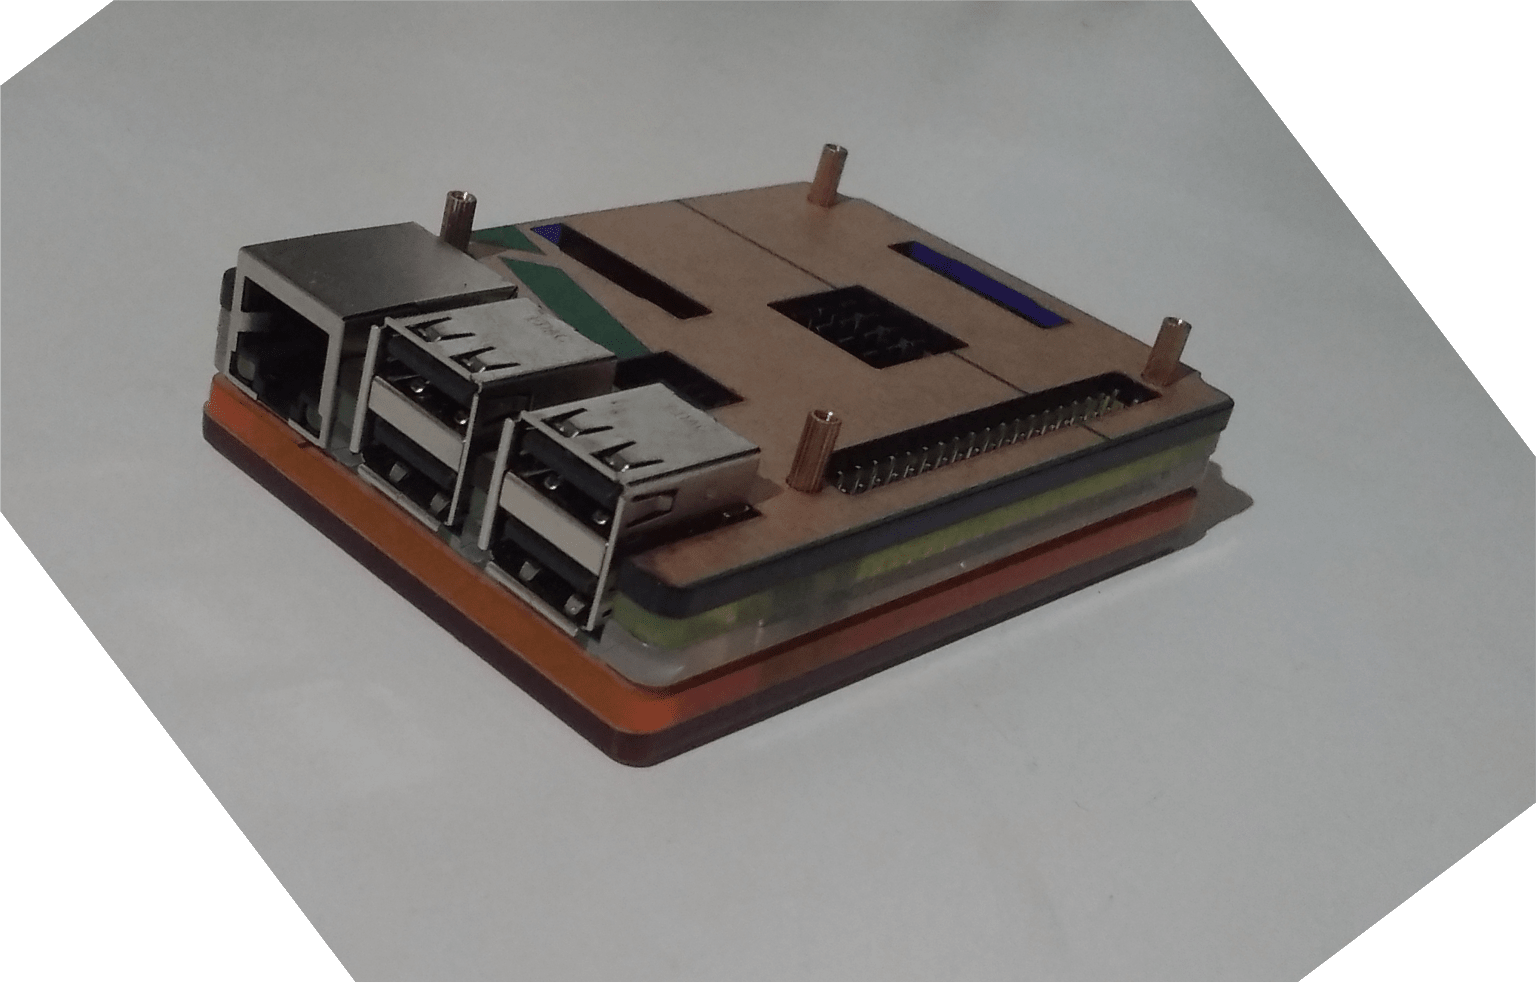
\includegraphics[scale=.20]{imagens/raspberry-min.png}}\\
\makebox[\width]{Fonte: foto tirada pelo autor} \label{Fig:raspberry_pi}
\end{figure}

O \textit{Raspberry Pi}, segundo \citeonline{oliveira}, é um computador montado em apenas uma única placa, o qual se classifica como \textit{Single-Board Computer (SBC)}. Ele ainda afirma que nesta placa, são integrados o processador, memória, portas de I/O e outros componentes que são necessários para seu funcionamento. A arquitetura presente em seu processador é um ARM, semelhantes aos processadores utilizados em celulares, tablets ou sistemas embarcados. \citeonline{richardsonwallace} afirmam que este processador é o mesmo que os encontrados no iPhone 3G e no \textit{Kindle} 2, o que permite ter uma referência sobre seu poder de processamento. De acordo com os autores, os chips ARM possuem diferentes núcleos configurados para fornecer capacidades diferentes de processamento. Seu sistema operacional padrão é uma distribuição Linux conhecida como \textit{Raspbian}, entretanto, os autores ressaltam que o usuário final não é limitado a utilizar somente este S.O. no dispositivo, ficando livre para explorar outras distribuições.

\section{COMPUTAÇÃO EM NUVEM}
De acordo com a definição da \citeonline{microsoft}, computação em nuvem é a disponibilização de diversos serviços de computação - como servidores, armazenamento, banco de dados, sistemas, entre outros serviços de TI - através da internet. A \textit{Amazon Web Service} \nocite{amazoncloudcomputing} ainda complementa que a plataforma que provê estes serviços é responsável pela manutenção de todo equipamento necessário para a disponibilização dos serviços. Tanto a \textit{Amazon Web Services (AWS)} quanto a Microsoft \textit{Azure} são plataformas conhecidas que proveem serviços de computação em nuvem.

Ambas afirmam que existem vários benefícios na utilização destes serviços. Dentre eles, uma das vantagens é relacionada ao custo, pois dispensa o gasto com qualquer tipo de equipamento para manter um datacenter local, uma vez que é utilizado uma infraestrutura já pronta e montada por estas prestadoras de serviço, que garantem a disponibilidade dos recursos através da internet \cite{amazoncloudcomputing, microsoft}.

Estes serviços são classificados em três tipos: Infraestrutura como Serviço (IaaS), Plataforma como Serviço (PaaS) e Software como Serviço (SaaS). A categoria de IaaS, segundo a definição da \citeonline{microsoft}, é a mais básica e provém toda a infraestrutura de TI, como servidores, máquinas virtuais, armazenamento, redes e sistemas operacionais. A categoria PaaS são serviços de computação que fornecem ambientes sob demanda para desenvolvimento, teste, fornecimento e gerenciamento de aplicativos de software. O SaaS fornece aplicativos de software pela nuvem sob demanda, normalmente baseadas em assinaturas.

\section{INTERNET DAS COISAS \textit{(INTERNET OF THINGS - IOT)}}
A ideia de \textit{IoT} se refere aos objetos do mundo físico gerando informações de forma autônoma para os computadores \cite{ashton}. Ele reforça que todas as informações presentes na internet foram geradas a partir de um ser humano. Uma questão pontuada por ele é referida à limitação das pessoas com relação ao tempo, atenção e precisão. Essa limitação pode resultar em ineficiência ao capturar dados sobre o mundo real. Dito isso, o autor conclui afirmando que é necessário capacitar os computadores através de seus próprios meios de coleta de informações para observarem e compreenderem o mundo físico sem a limitação da entrada de dados através de uma pessoa.

O conceito de Internet das Coisas conforme definido pelo projeto \citeonline{casagras} na introdução e idealizado por \citeonline{ashton} abordam a interconectividade e troca de informações entre os objetos do mundo físico com o mundo virtual (Figura \ref{Fig:representacao_iot}). \citeonline{dias} afirma que existem infinitas possibilidades de negócio e aplicações envolvendo o conceito de internet das coisas. Ela ainda menciona alguns nichos destes negócios, como os voltados para os bens de consumo, distribuição de energia, casas inteligentes, indústria e manufatura e transporte inteligente. Para este último nicho, a autora ainda traz algumas aplicações possíveis de serem exploradas, como notificação das condições de tráfego, controle inteligente de rotas, coordenação das rodovias e monitoramento remoto de veículos.

\begin{figure}[!ht]
\centering
\caption{Representação da interação das 'coisas' dentro do conceito de \textit{IoT}.} 
{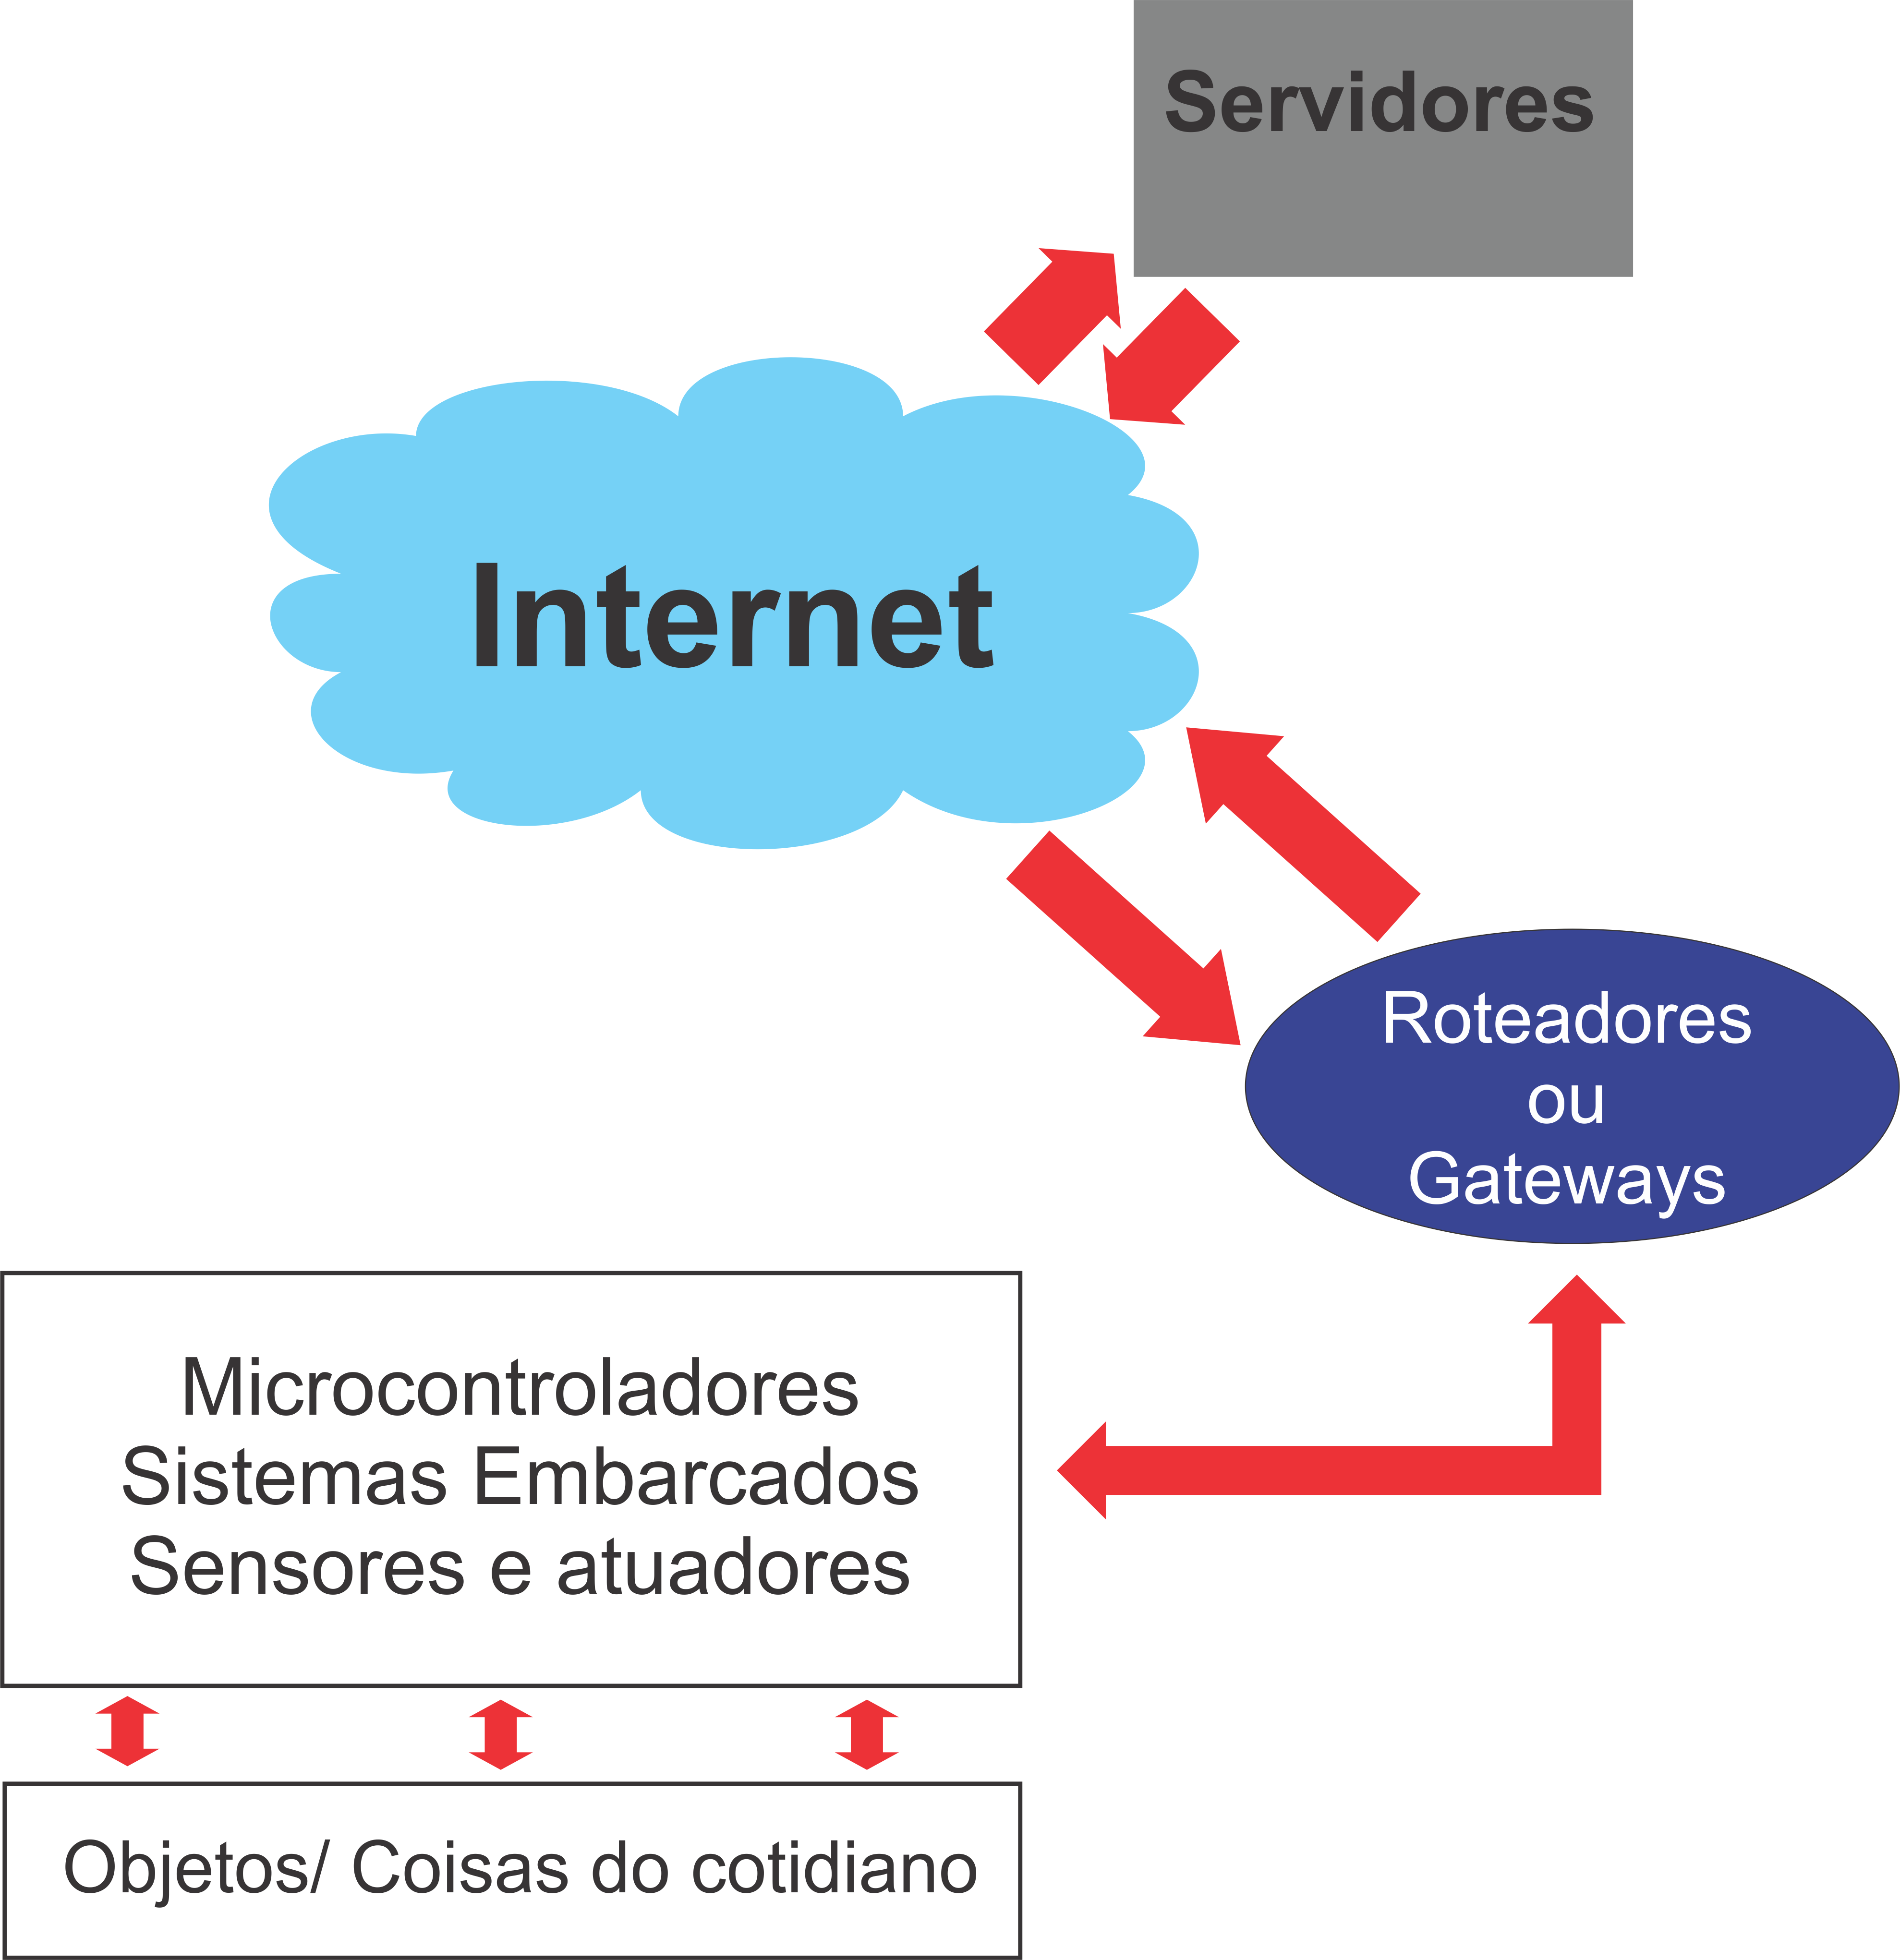
\includegraphics[scale=.40]{imagens/diagramaIOT.png}}\\
\makebox[\width]{Fonte: baseado nas obras de \citeonline{ashton}, \citeonline{casagras} e \citeonline{dias}} \label{Fig:representacao_iot}
\end{figure}

De acordo com o que foi apresentado até o momento, observam-se dois pontos importantes: primeiro, a cada evolução de um automóvel, nota-se que ele está se tornando mais informatizado e conectado; segundo, a tendência da \textit{IoT} é permitir que cada vez mais as coisas se comuniquem e troquem informações entre si, com mínima intervenção humana.

\chapter{METODOLOGIA}\label{CAP5}

O desenvolvimento do trabalho foi dividido em 3 etapas. A primeira etapa consistiu no desenvolvimento do software responsável por fazer a interação com a rede interna automotiva. A segunda etapa foi caracterizada pela configuração do \textit{Raspberry Pi} e instalação do software no dispositivo e a terceira etapa se refere à integração da aplicação com um serviço de computação em nuvem.

\section{DESENVOLVIMENTO DO SOFTWARE DE LEITURA}
O objetivo principal da concepção do software nesta fase inicial é possibilitar ao computador interagir com a rede interna veicular, enviando e recebendo dados através da interface \textit{OBD-II}. Para permitir a tradução de protocolos e tornar a comunicação simplificada, foi adquirido o dispositivo ELM327 com transmissão \textit{Bluetooth}, responsável por tratar das conversões dos protocolos automotivos presentes no conector \textit{OBD-II} para uma interface serial padrão, estabelecendo uma comunicação com o adaptador \textit{Bluetooth} do computador.

A construção do software foi feita utilizando-se a linguagem de programação Java na versão 8, juntamente com as seguintes tecnologias: \textit{BlueCove}, obd-java-api e JavaFx. \textit{BlueCove} é uma biblioteca Java que segue a especificação JSR-82, permitindo que uma aplicação acesse o adaptador \textit{Bluetooth} local para se comunicar com outros dispositivos \cite{bluecove}. obd-java-api, encontrada no repositório de Pires (https://github.com/pires/obd-java-api), é uma biblioteca que facilita a comunicação com o adaptador ELM327. O \textit{framework} JavaFx fornece um conjunto de pacotes que facilitam a criação de uma interface gráfica para uma aplicação \cite{pawlan}. A Figura \ref{Fig:tela_leitura_javafx} representa o protótipo do software desenvolvido utilizando o JavaFx.

\begin{figure}[!ht]
\centering
\caption{Imagem da tela de leitura prototipada.} 
{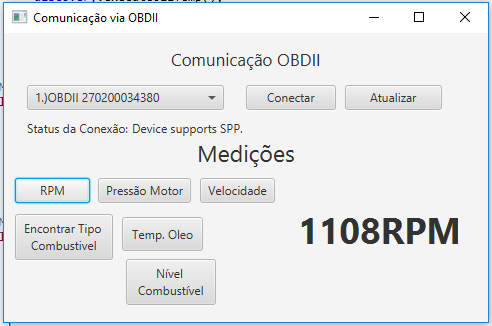
\includegraphics[scale=.75]{imagens/telaLeituraJavaFx.png}}\\
\makebox[\width]{Fonte: produzido pelo autor} \label{Fig:tela_leitura_javafx}
\end{figure}

\subsection{\textbf{Arquitetura do software}}
O projeto foi desenvolvido utilizando-se o paradigma de programação orientada à objeto e o padrão \textit{Model-View-Controller (MVC)}, e devido a isso, foi necessário criar cinco pacotes para organizar as classes do código fonte. Os nomes dos pacotes criados foram: \textit{app}, \textit{bluetooth}, \textit{controller}, \textit{scanner}, e \textit{view}.

No pacote \textit{app} contém a classe \textit{AppStart} que é responsável por iniciar a aplicação e carregar a interface de usuário \textit{ScreenMonitor} contida no pacote \textit{view}. O pacote \textit{bluetooth} contém duas classes, uma chamada \textit{DiscoveryDevices} – responsável pela descoberta de dispositivos \textit{bluetooth} próximos – e outra chamada \textit{BluetoothConnection}, responsável por obter uma conexão \textit{bluetooth}. Dentro do pacote \textit{scanner} existem duas classes, uma com o nome \textit{ConnectToDevice}, que é responsável por estabelecer uma conexão com o dispositivo ELM327, e outra com o nome ELM327, representando o próprio dispositivo. O pacote \textit{view} contém o arquivo \textit{ScreenMonitor} no formato FXML, responsável por representar a interface de usuário. Por fim, o pacote \textit{controller} contém a classe \textit{ScreenMonitorController}, responsável por receber as entradas do usuário na interface e mapear as ações a serem tomadas pelo software. Na Figura \ref{Fig:diagrama_classe}, é possível observar a organização e estruturação das classes no projeto. A implementação do código das classes dos pacotes \textit{bluetooth} e \textit{scanner} poderá ser consultado em detalhes em Anexo.

\begin{figure}[!ht]
\centering
\caption{Diagrama de pacote exibindo a estrutura de pacotes do projeto com as respectivas classes.} 
{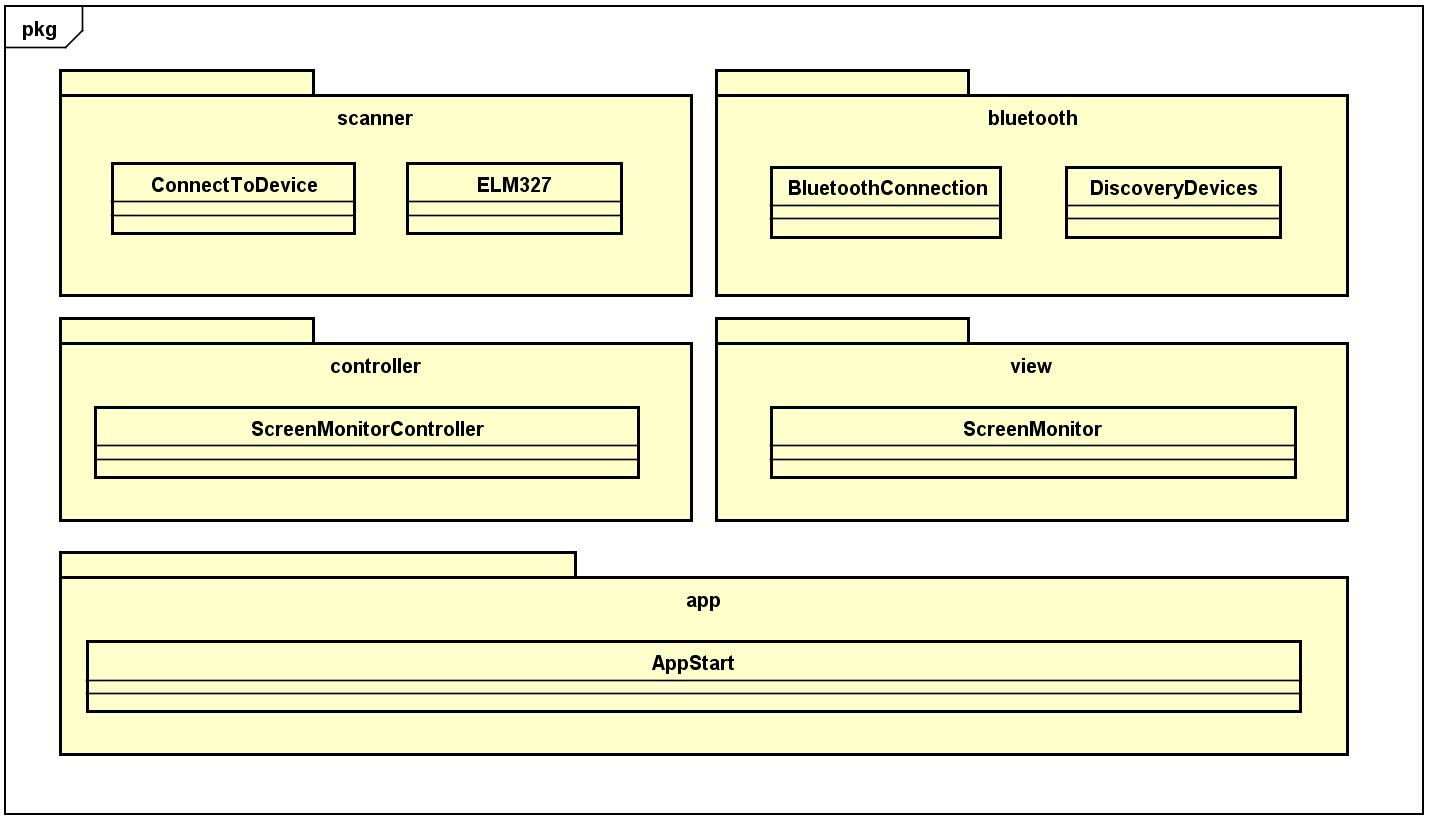
\includegraphics[scale=.42]{imagens/estruturacaoPacotes.png}}\\
\makebox[\width]{Fonte: produzido pelo autor} \label{Fig:diagrama_classe}
\end{figure}

No pacote \textit{scanner} existe a classe ELM327 (Figura \ref{Fig:elm327_class}) responsável por estabelecer a comunicação com o dispositivo de mesmo nome. Essa classe recebe como parâmetro em seu construtor dois objetos do tipo \textit{InputStream} e \textit{OutputStream}. Ela também contém alguns métodos, que são: \textit{disconnect} (Figura \ref{Fig:elm327_disconnect}), responsável por fechar a conexão dos objetos \textit{InputStream} e \textit{OutputStream}; \textit{readRpm} (Figura \ref{Fig:elm327_read_rpm}), responsável por efetuar a leitura da rotação por minuto (RPM) do motor, devolvendo uma \textit{string} no formato correto; \textit{readSpeed} (Figura \ref{Fig:elm327_read_speed}), responsável por efetuar a leitura da velocidade atual do automóvel, também retornando uma \textit{string} no formato Km/h; \textit{readFuelPressure} (Figura \ref{Fig:elm327_read_fuel_pressure}), responsável por obter a pressão do combustível em uma \textit{string}, no formato Psi ou Kilopascal (kPa); \textit{readOilTemp} (Figura \ref{Fig:elm327_read_oil_temp}), responsável por ler a temperatura do óleo do motor e devolver uma \textit{string} com o valor em graus \textit{Celsius} ($^{\circ}$C); \textit{readFindFuelType} (Figura \ref{Fig:elm327_read_find_fuel_type}), responsável por encontrar qual tipo de combustível está sendo utilizado no tanque; \textit{readFuelLevel} (Figura \ref{Fig:elm327_read_fuel_level}), responsável por obter a informação referente ao nível de combustível presente no tanque, e por último, o método \textit{clearBuffer} (Figura \ref{Fig:elm327_clear_buffer}), que implementa vários comandos que reiniciam a conexão \textit{OBD}, limpam o eco e o cabeçalho, possibilitando apagar o \textit{buffer} presente no dispositivo ELM327 para realizar novas leituras. Todos os métodos pertencentes à esta classe, exceto o \textit{disconnect}, fazem uso de classes e métodos que pertencem à biblioteca obd-java-api. Desta forma, as classes e métodos contidos nesta biblioteca abstraem a implementação de comandos ‘AT’ e \textit{‘OBD’}, tornando a sua utilização simplificada, bastando apenas chamar o recurso a ser utilizado sem se preocupar com a forma de implementação da funcionalidade.

\begin{figure}[!ht]
\centering
\caption{Foto da classe ELM327.} 
{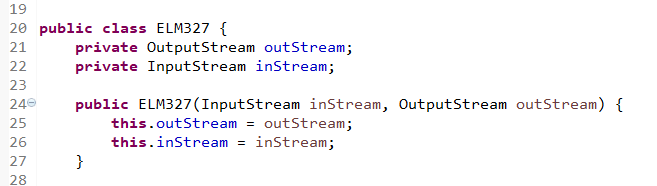
\includegraphics[scale=.70]{imagens/pacoteScanner-ELM327.png}}\\
\makebox[\width]{Fonte: produzido pelo autor} \label{Fig:elm327_class}
\end{figure}

\begin{figure}[!ht]
\centering
\caption{Foto do método \textit{disconnect} da classe ELM327.} 
{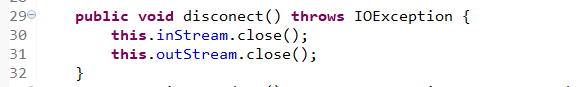
\includegraphics[scale=.70]{imagens/pacoteScanner-ELM327_disconnect.png}}\\
\makebox[\width]{Fonte: produzido pelo autor} \label{Fig:elm327_disconnect}
\end{figure}

\begin{figure}[!ht]
\centering
\caption{Foto do método \textit{readRpm} da classe ELM327.} 
{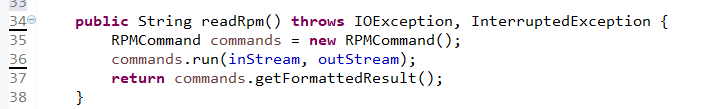
\includegraphics[scale=.85]{imagens/pacoteScanner-ELM327_readRpm.png}}\\
\makebox[\width]{Fonte: produzido pelo autor} \label{Fig:elm327_read_rpm}
\end{figure}

\begin{figure}[!ht]
\centering
\caption{Foto do método \textit{readSpeed} da classe ELM327.} 
{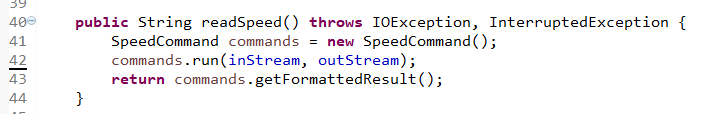
\includegraphics[scale=.85]{imagens/pacoteScanner-ELM327_readSpeed.png}}\\
\makebox[\width]{Fonte: produzido pelo autor} \label{Fig:elm327_read_speed}
\end{figure}

\begin{figure}[!ht]
\centering
\caption{Foto do método \textit{readFuelPressure} da classe ELM327.} 
{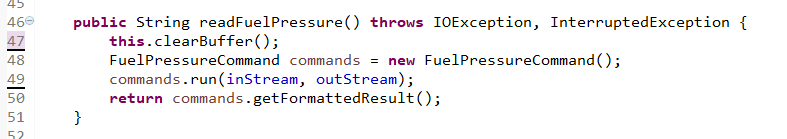
\includegraphics[scale=.80]{imagens/pacoteScanner-ELM327_readFuelPressure.png}}\\
\makebox[\width]{Fonte: produzido pelo autor} \label{Fig:elm327_read_fuel_pressure}
\end{figure}

\begin{figure}[!ht]
\centering
\caption{Foto do método \textit{readOilTemp} da classe ELM327.} 
{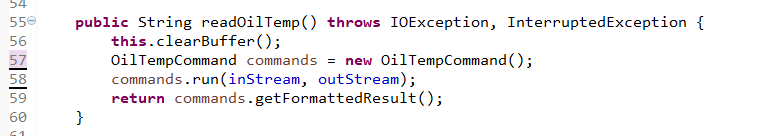
\includegraphics[scale=.85]{imagens/pacoteScanner-ELM327_readOilTemp.png}}\\
\makebox[\width]{Fonte: produzido pelo autor} \label{Fig:elm327_read_oil_temp}
\end{figure}

\begin{figure}[!ht]
\centering
\caption{Foto do método \textit{readFindFuelType} da classe ELM327.} 
{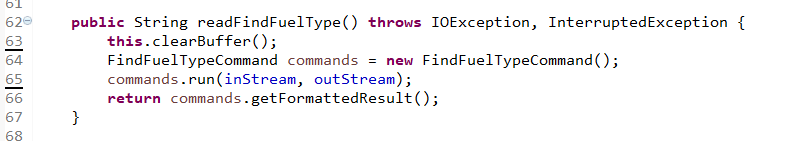
\includegraphics[scale=.80]{imagens/pacoteScanner-ELM327_readFindFuelType.png}}\\
\makebox[\width]{Fonte: produzido pelo autor} \label{Fig:elm327_read_find_fuel_type}
\end{figure}

\begin{figure}[!ht]
\centering
\caption{Foto do método \textit{readFuelLevel} da classe ELM327.} 
{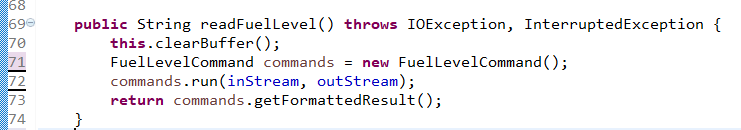
\includegraphics[scale=.70]{imagens/pacoteScanner-ELM327_readFuelLevel.png}}\\
\makebox[\width]{Fonte: produzido pelo autor} \label{Fig:elm327_read_fuel_level}
\end{figure}

\begin{figure}[!ht]
\centering
\caption{Foto do método \textit{clearBuffer} da classe ELM327.} 
{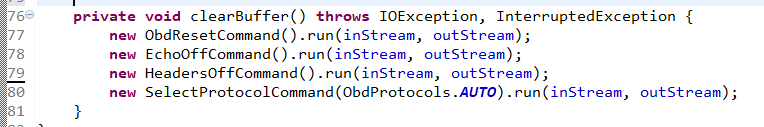
\includegraphics[scale=.70]{imagens/pacoteScanner-ELM327_clearBuffer.png}}\\
\makebox[\width]{Fonte: produzido pelo autor} \label{Fig:elm327_clear_buffer}
\end{figure}

Os pacotes \textit{view}, e \textit{controller} são implementações da arquitetura \textit{MVC}, que correspondem respectivamente à arquivos relacionados à interface de usuário, e à classes responsáveis por administrar as entradas dos usuários. Segundo \citeonline{medeirosmvc}, a arquitetura \textit{MVC} possui o controlador \textit{(Controller)} que gerencia as entradas dos usuários através das visões \textit{(Views)}, passando os comandos para os modelos \textit{(Models)} que gerencia diversos elementos de dados. Seguindo esta ideia, os pacotes que tem o papel de modelo, segundo esta arquitetura, seria o \textit{scanner} e o \textit{bluetooth} (Figura \ref{Fig:diagrama_mvc}).

\begin{figure}[!ht]
\centering
\caption{Representação da arquitetura \textit{MVC} do projeto.} 
{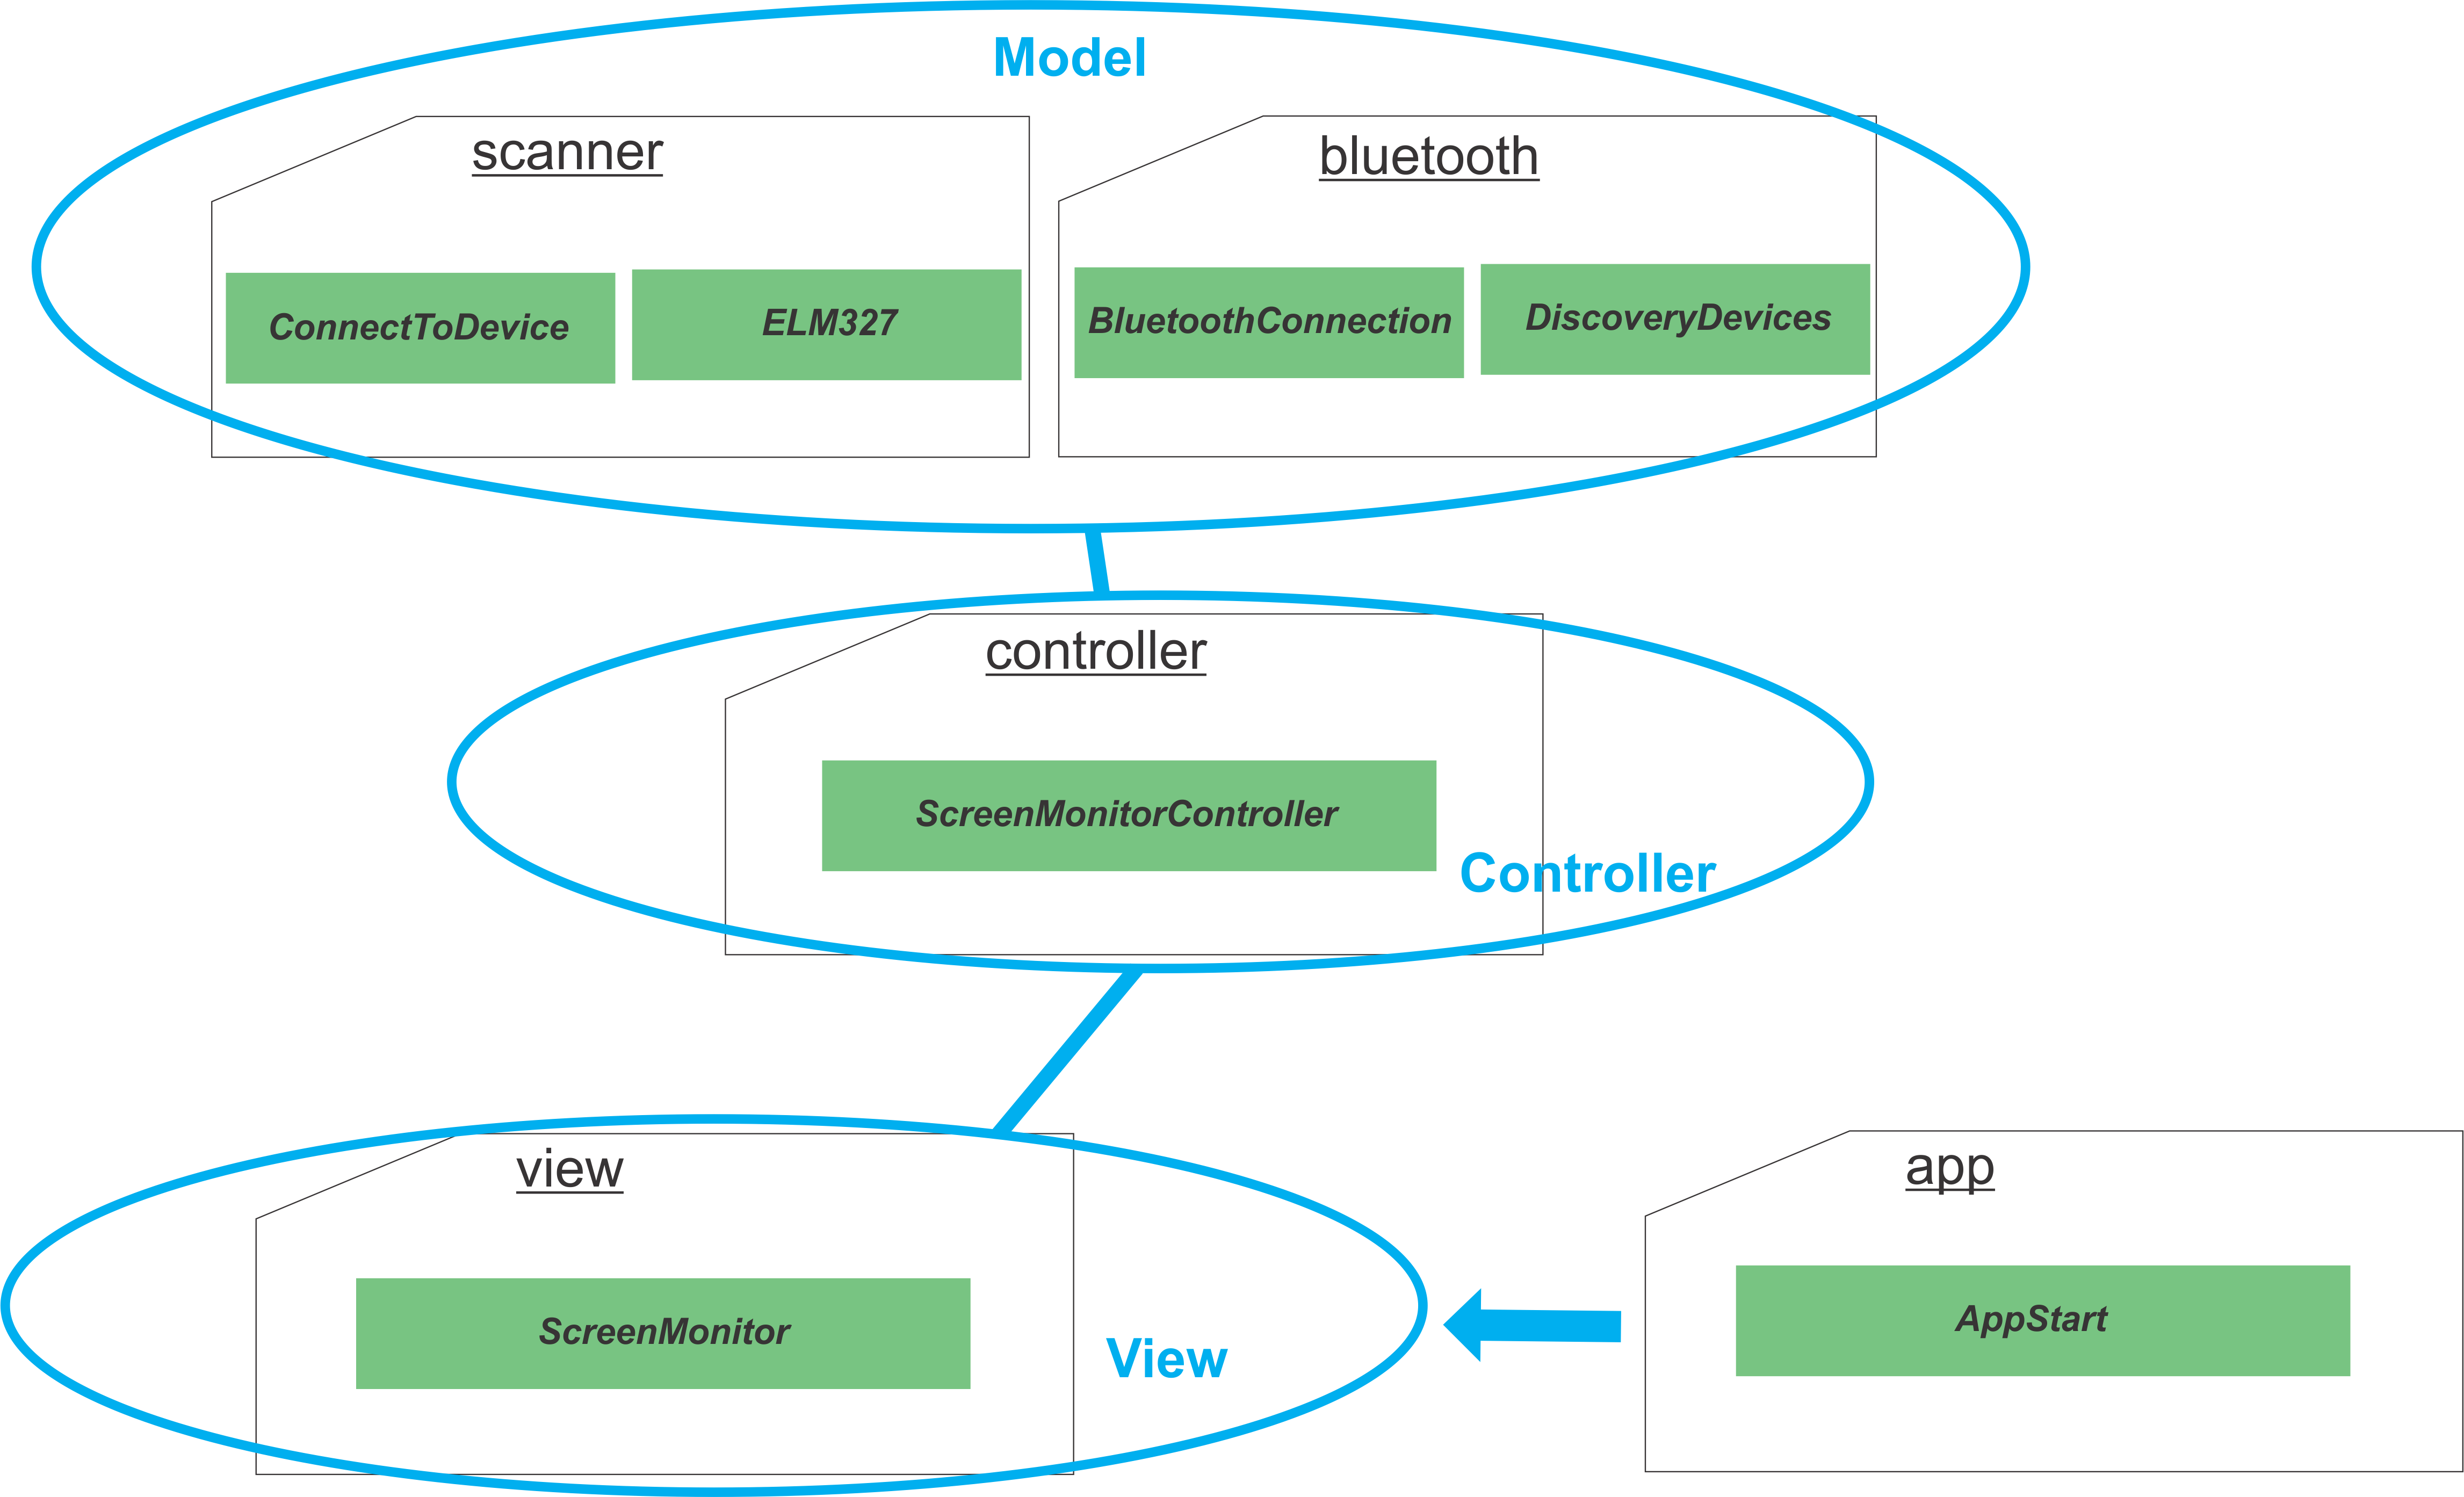
\includegraphics[scale=.40]{imagens/diagramaMvc.png}}\\
\makebox[\width]{Fonte: produzido pelo autor} \label{Fig:diagrama_mvc}
\end{figure}

\section{CONFIGURAÇÃO DO \textit{RASPBERRY PI} E INSTALAÇÃO DO SOFTWARE}
Primeiramente foi instalado a versão \textit{Jessie} do \textit{Raspbian}, com a atualização de 05 de julho de 2017 disponível em https://downloads.raspberrypi.org/raspbian/images/raspbian-2017-07-05/. O \textit{Raspbian}, conforme menciona \citeonline{long}, é uma distribuição do Linux baseada no Debian. Foi adquirido também, para o \textit{Raspberry} o display de 3.2 polegadas, modelo 3.2inch RPi Display com resolução de 320x240 pixels (Figura \ref{Fig:raspberry_display}). Este display é conectado na porta genérica de entrada e saída do \textit{Raspbery Pi} (porta GPIO - Figura \ref{Fig:raspberry_gpio}). O \textit{driver} de instalação do display está disponível em https://www.waveshare.com/wiki/3.2inch\_RPi\_LCD\_(B). De acordo com as instruções de instalação presentes neste site, os \textit{drivers} não são compatíveis com sistemas instalados pelo NOOBS. O sistema NOOBS, segundo o \citeauthor{raspberrypifoundation}, é um instalador de sistema operacional que contém o \textit{Raspbian}.

\begin{figure}[!ht]
\centering
\caption{Foto do display do \textit{Raspberry Pi}.} 
{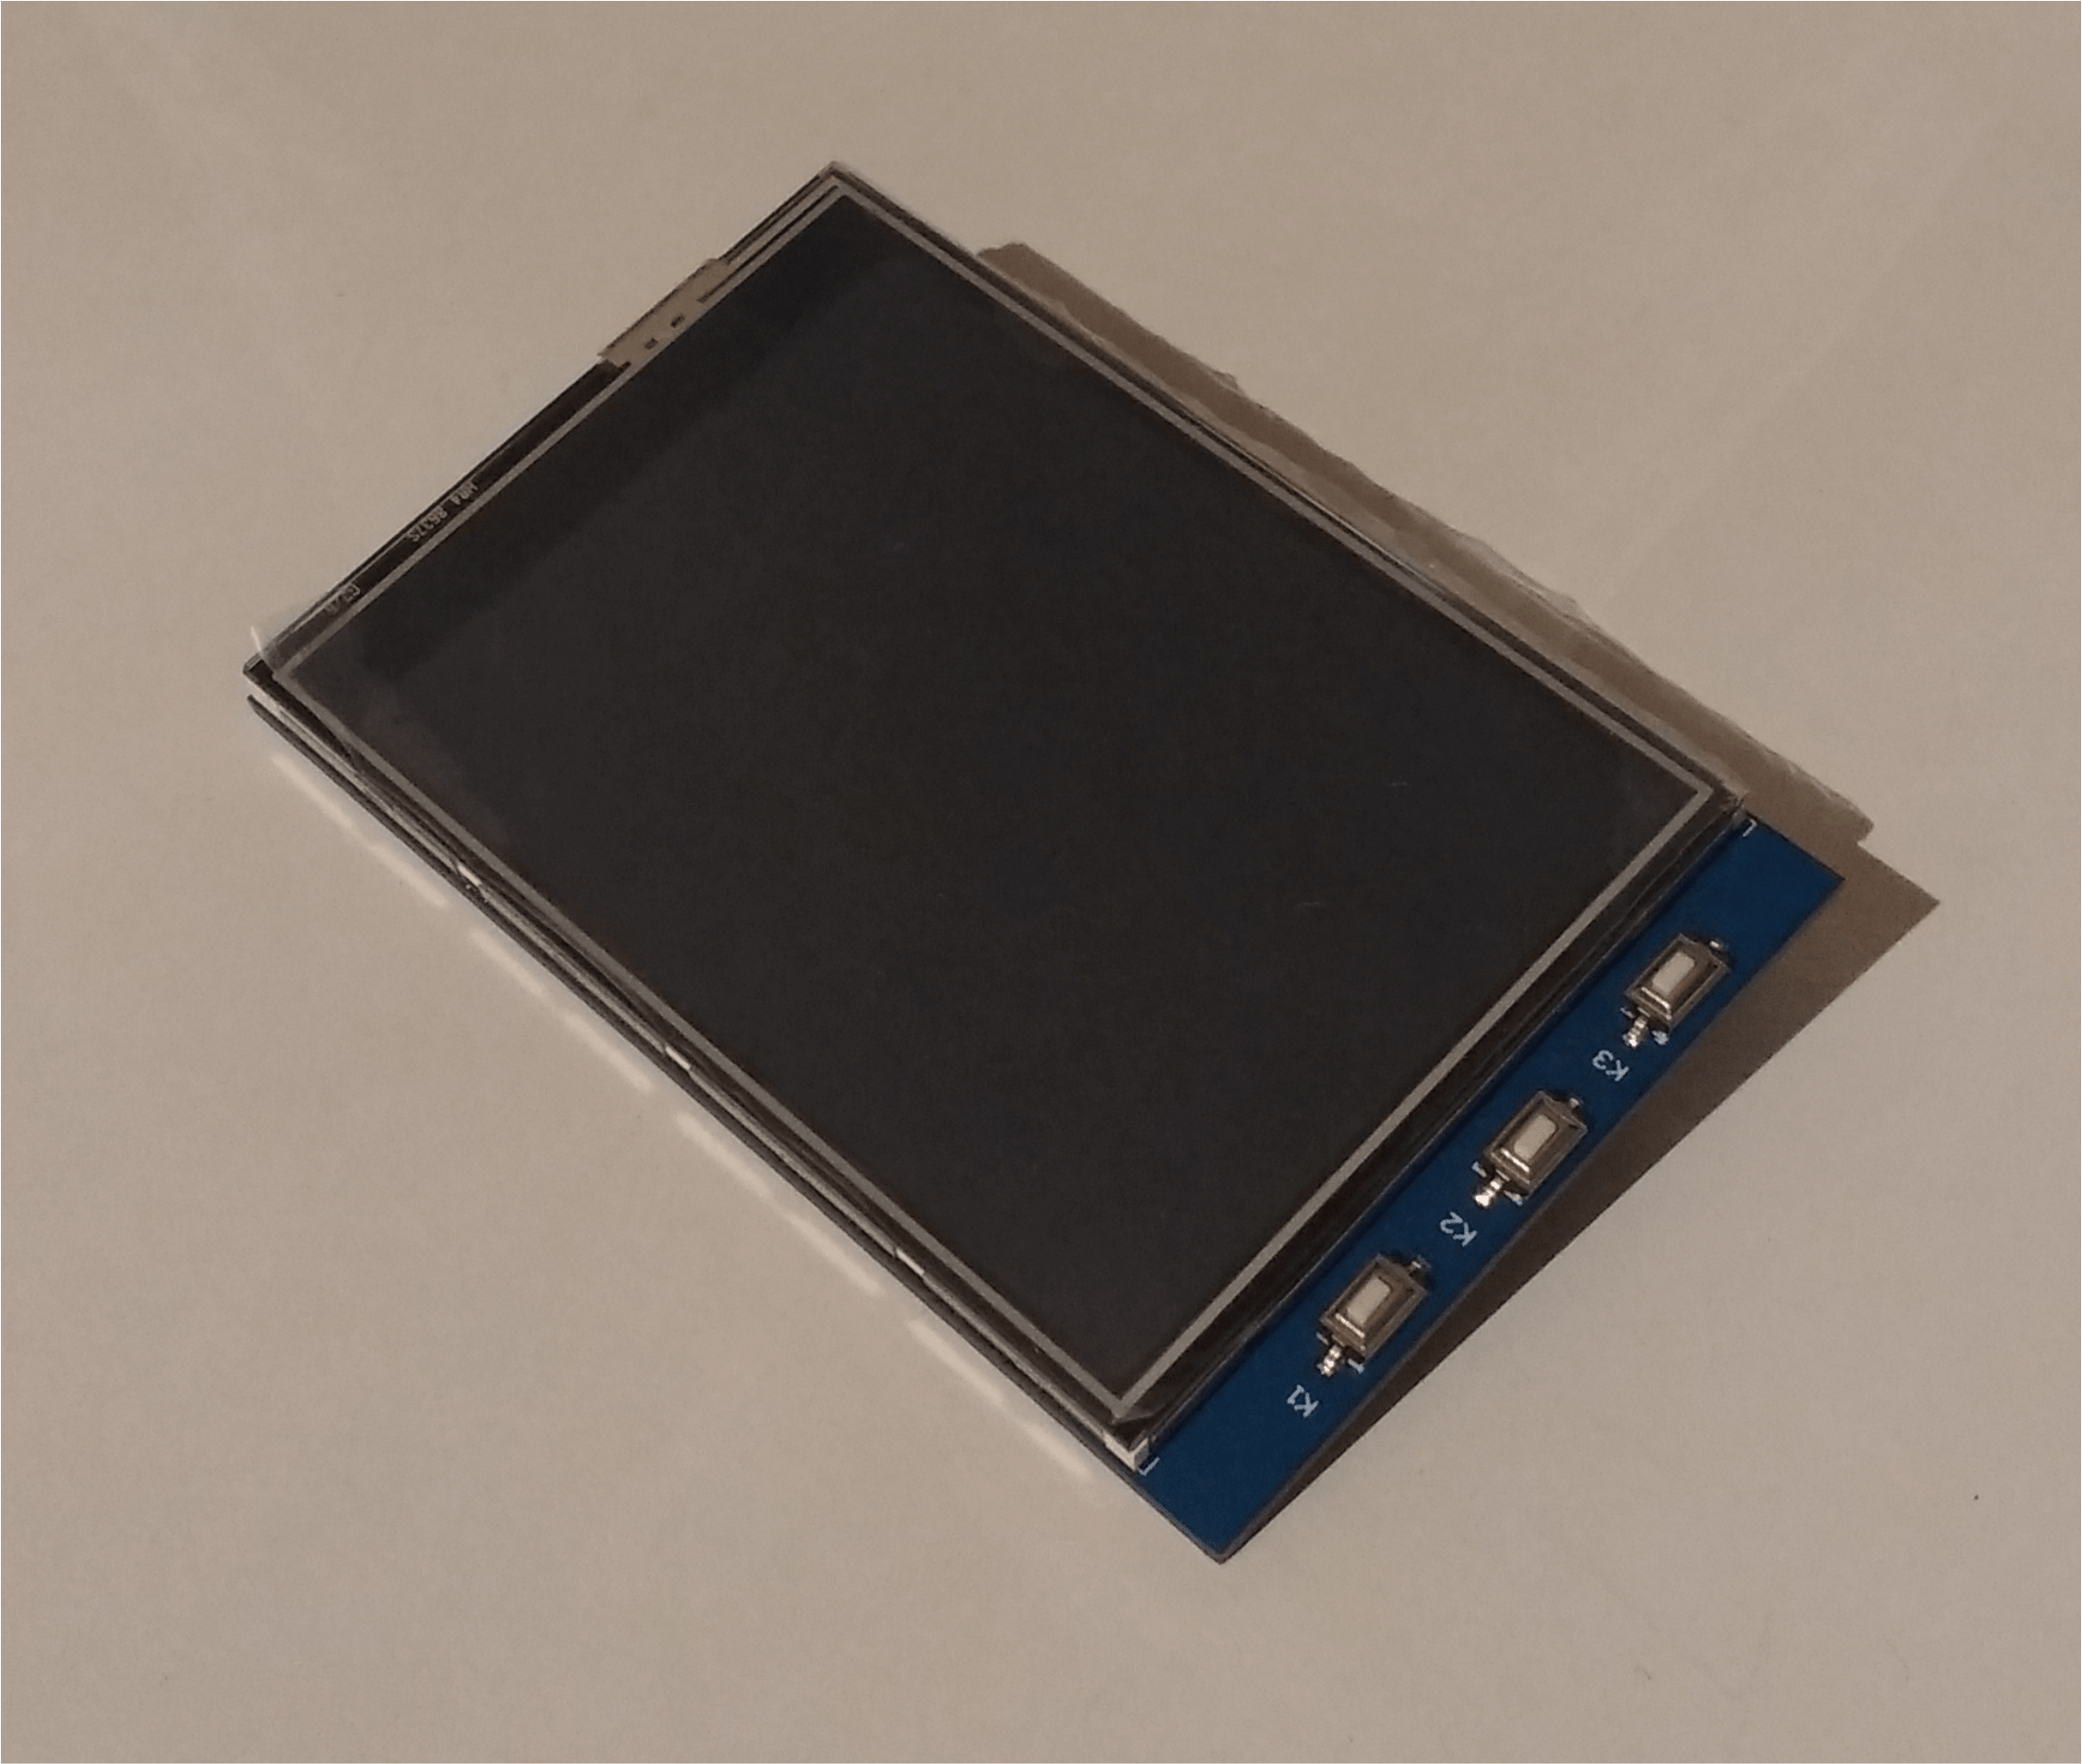
\includegraphics[scale=.12]{imagens/displayRaspberry-min.png}}\\
\makebox[\width]{Fonte: produzido pelo autor} \label{Fig:raspberry_display}
\end{figure}

\begin{figure}[!ht]
\centering
\caption{Porta GPIO do \textit{Raspberry Pi}.} 
{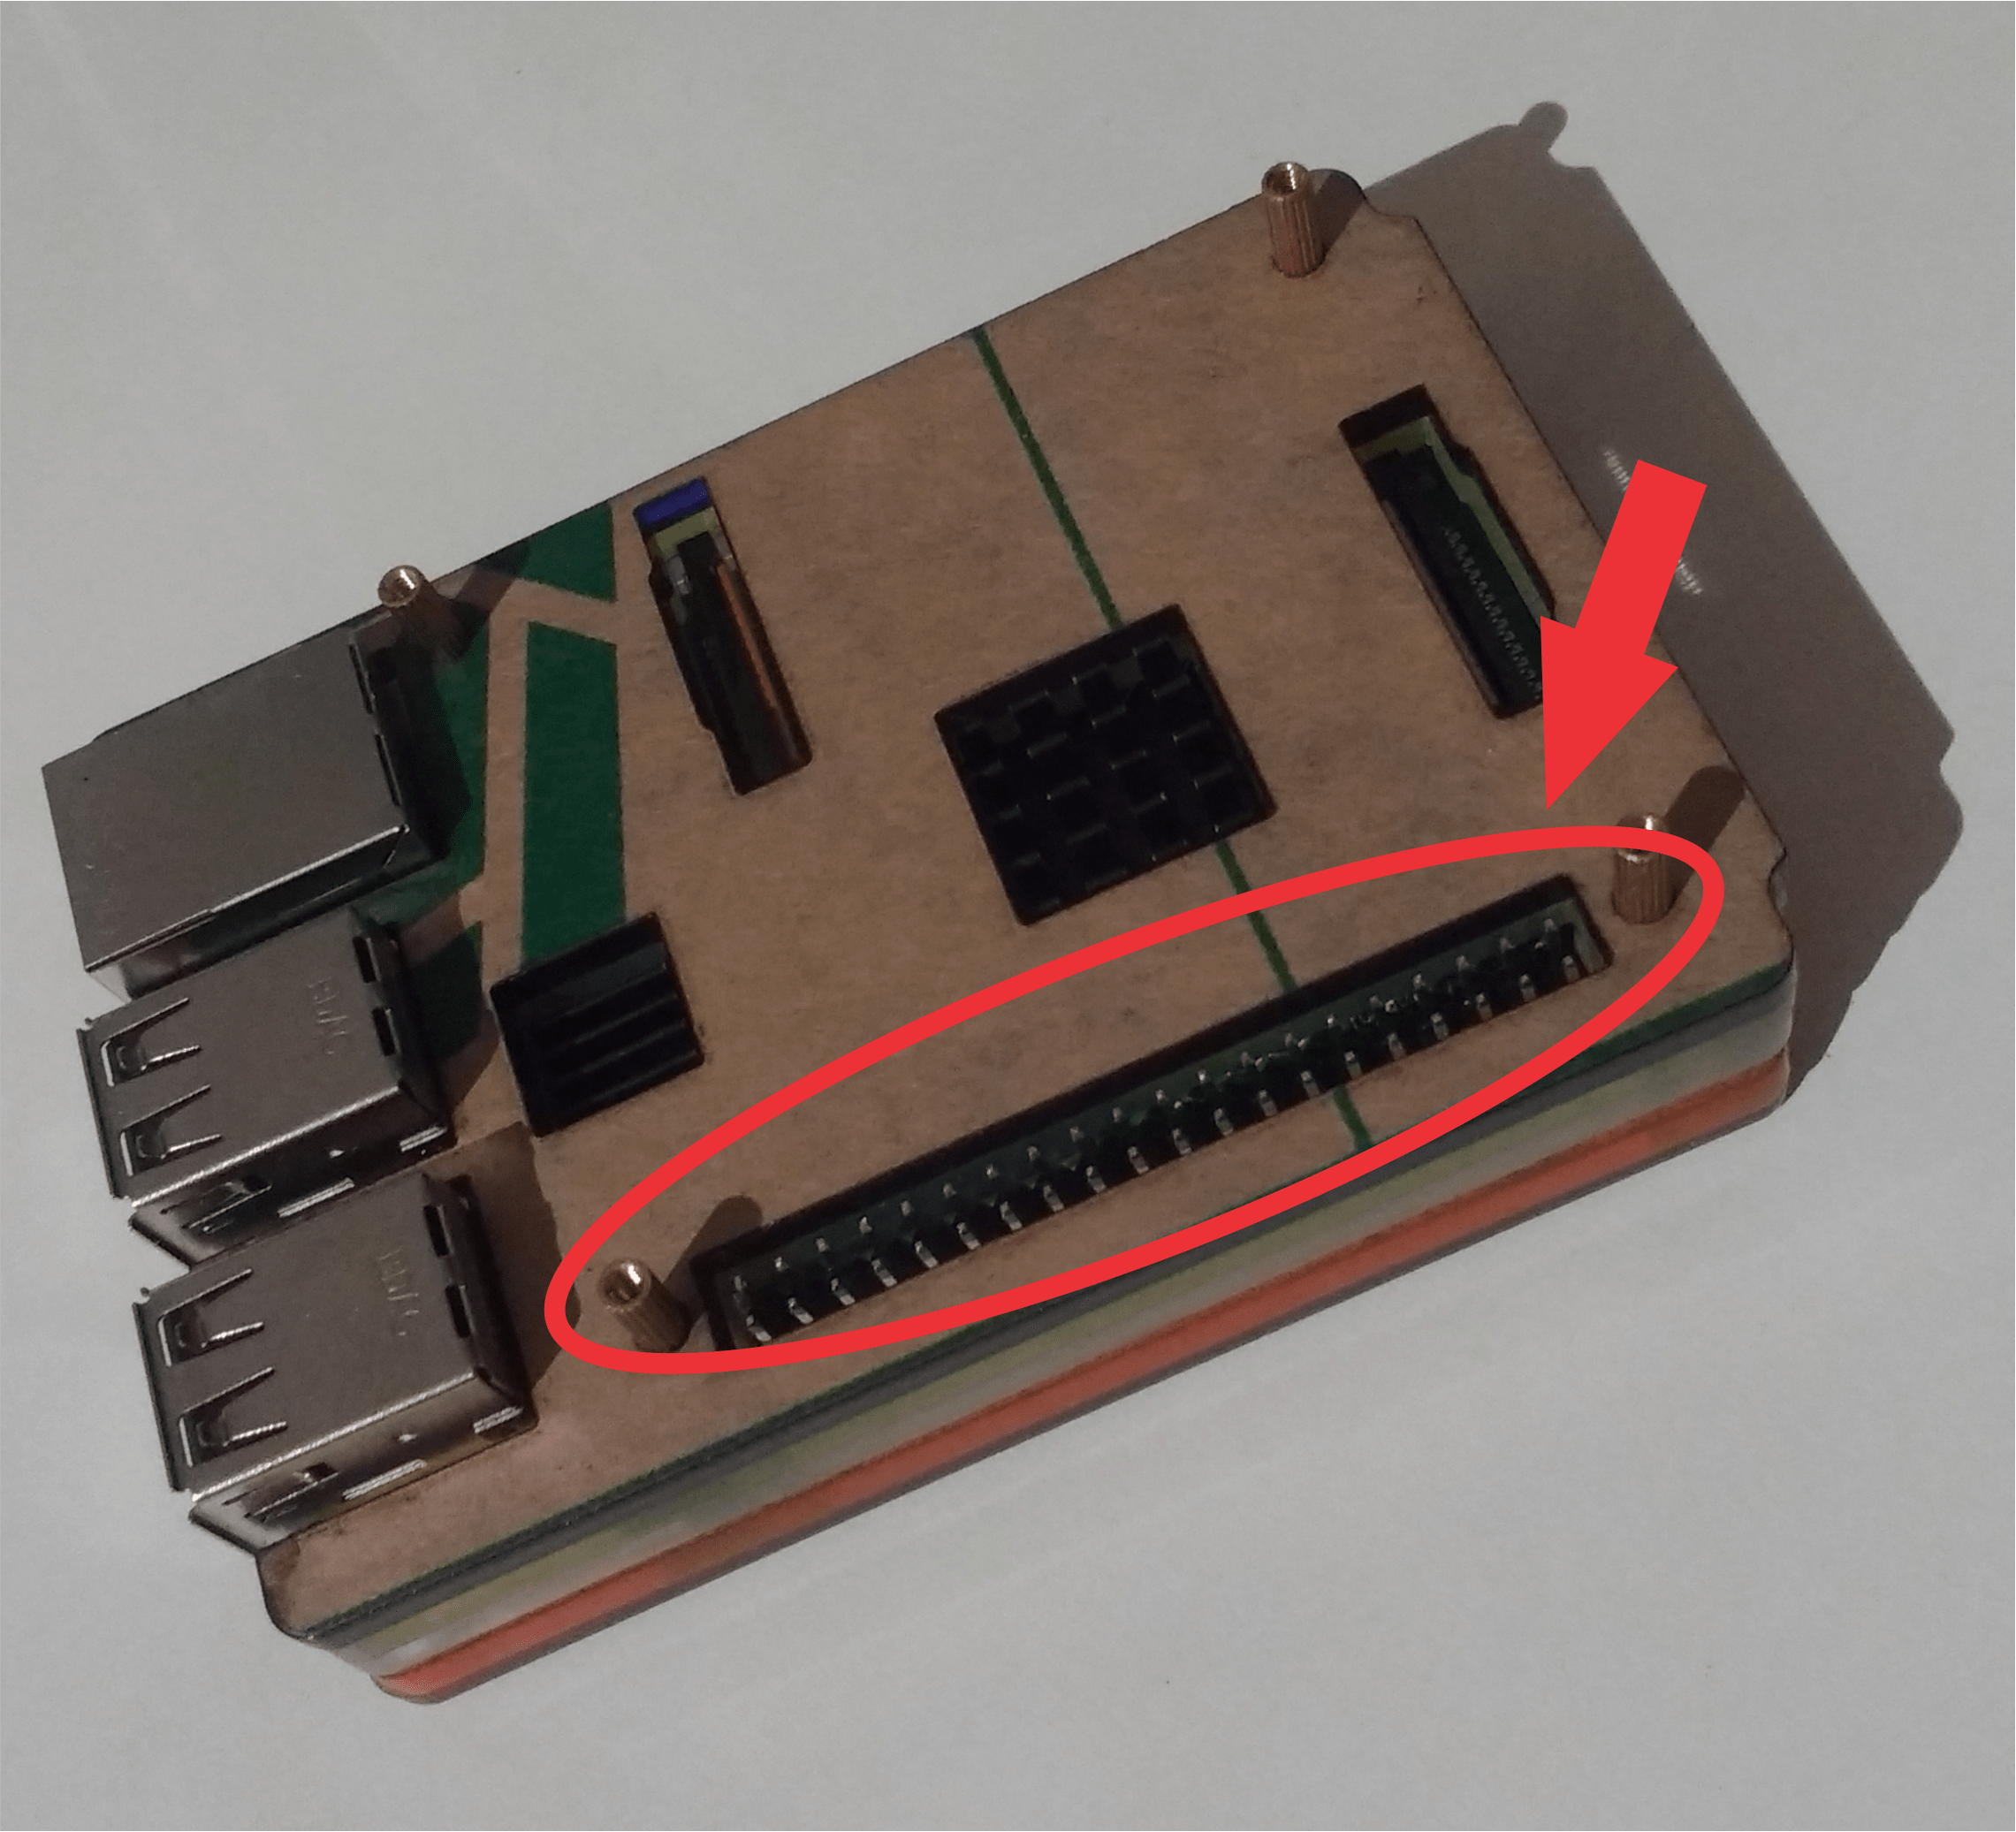
\includegraphics[scale=.12]{imagens/raspberryGPIO-min.png}}\\
\makebox[\width]{Fonte: produzido pelo autor} \label{Fig:raspberry_gpio}
\end{figure}

Para suportar a instalação e execução do software, depois de instalado e configurado o sistema operacional e o display, foi instalado o kit de desenvolvimento para Java na versão 8 (JDK 8) que incluía a máquina virtual (JRE) para rodar o projeto. Durante a fase de execução do projeto no ambiente do \textit{Raspberry}, notou-se que houve duas incompatibilidades. A primeira incompatibilidade identificada foi relacionada à biblioteca \textit{BlueCove}, pois ela não fornecia suporte para arquitetura ARM. A solução alternativa para contornar este problema foi encontrar uma versão da biblioteca construída para esta arquitetura. A segunda incompatibilidade foi relacionada ao \textit{framework} JavaFx, utilizado na interface gráfica. Foi identificado que nas configrações do \textit{Raspberry} não era possível executar o software utilizando esta tecnologia. Para solucionar este problema, foi necessário redesenhar a interface utilizando o \textit{Swing} – conjunto de componentes que permite a criação de interface gráfica –, que são inteiramente implementados na linguagem Java \cite{oracle}.

Foram feitas algumas modificações no projeto e na interface para se adequar à tela do \textit{Raspberry} de 3.2 polegadas. Como havia uma limitação de espaço de exibição no display, apenas as leituras de RPM, velocidade, tipo e pressão do combustível foram implementadas. A Figura \ref{Fig:raspberry_sistema} mostra o software adaptado à tela, sendo executado no \textit{Raspberry Pi}.

\begin{figure}[!ht]
\centering
\caption{Software sendo executado no \textit{Raspberry Pi}.} 
{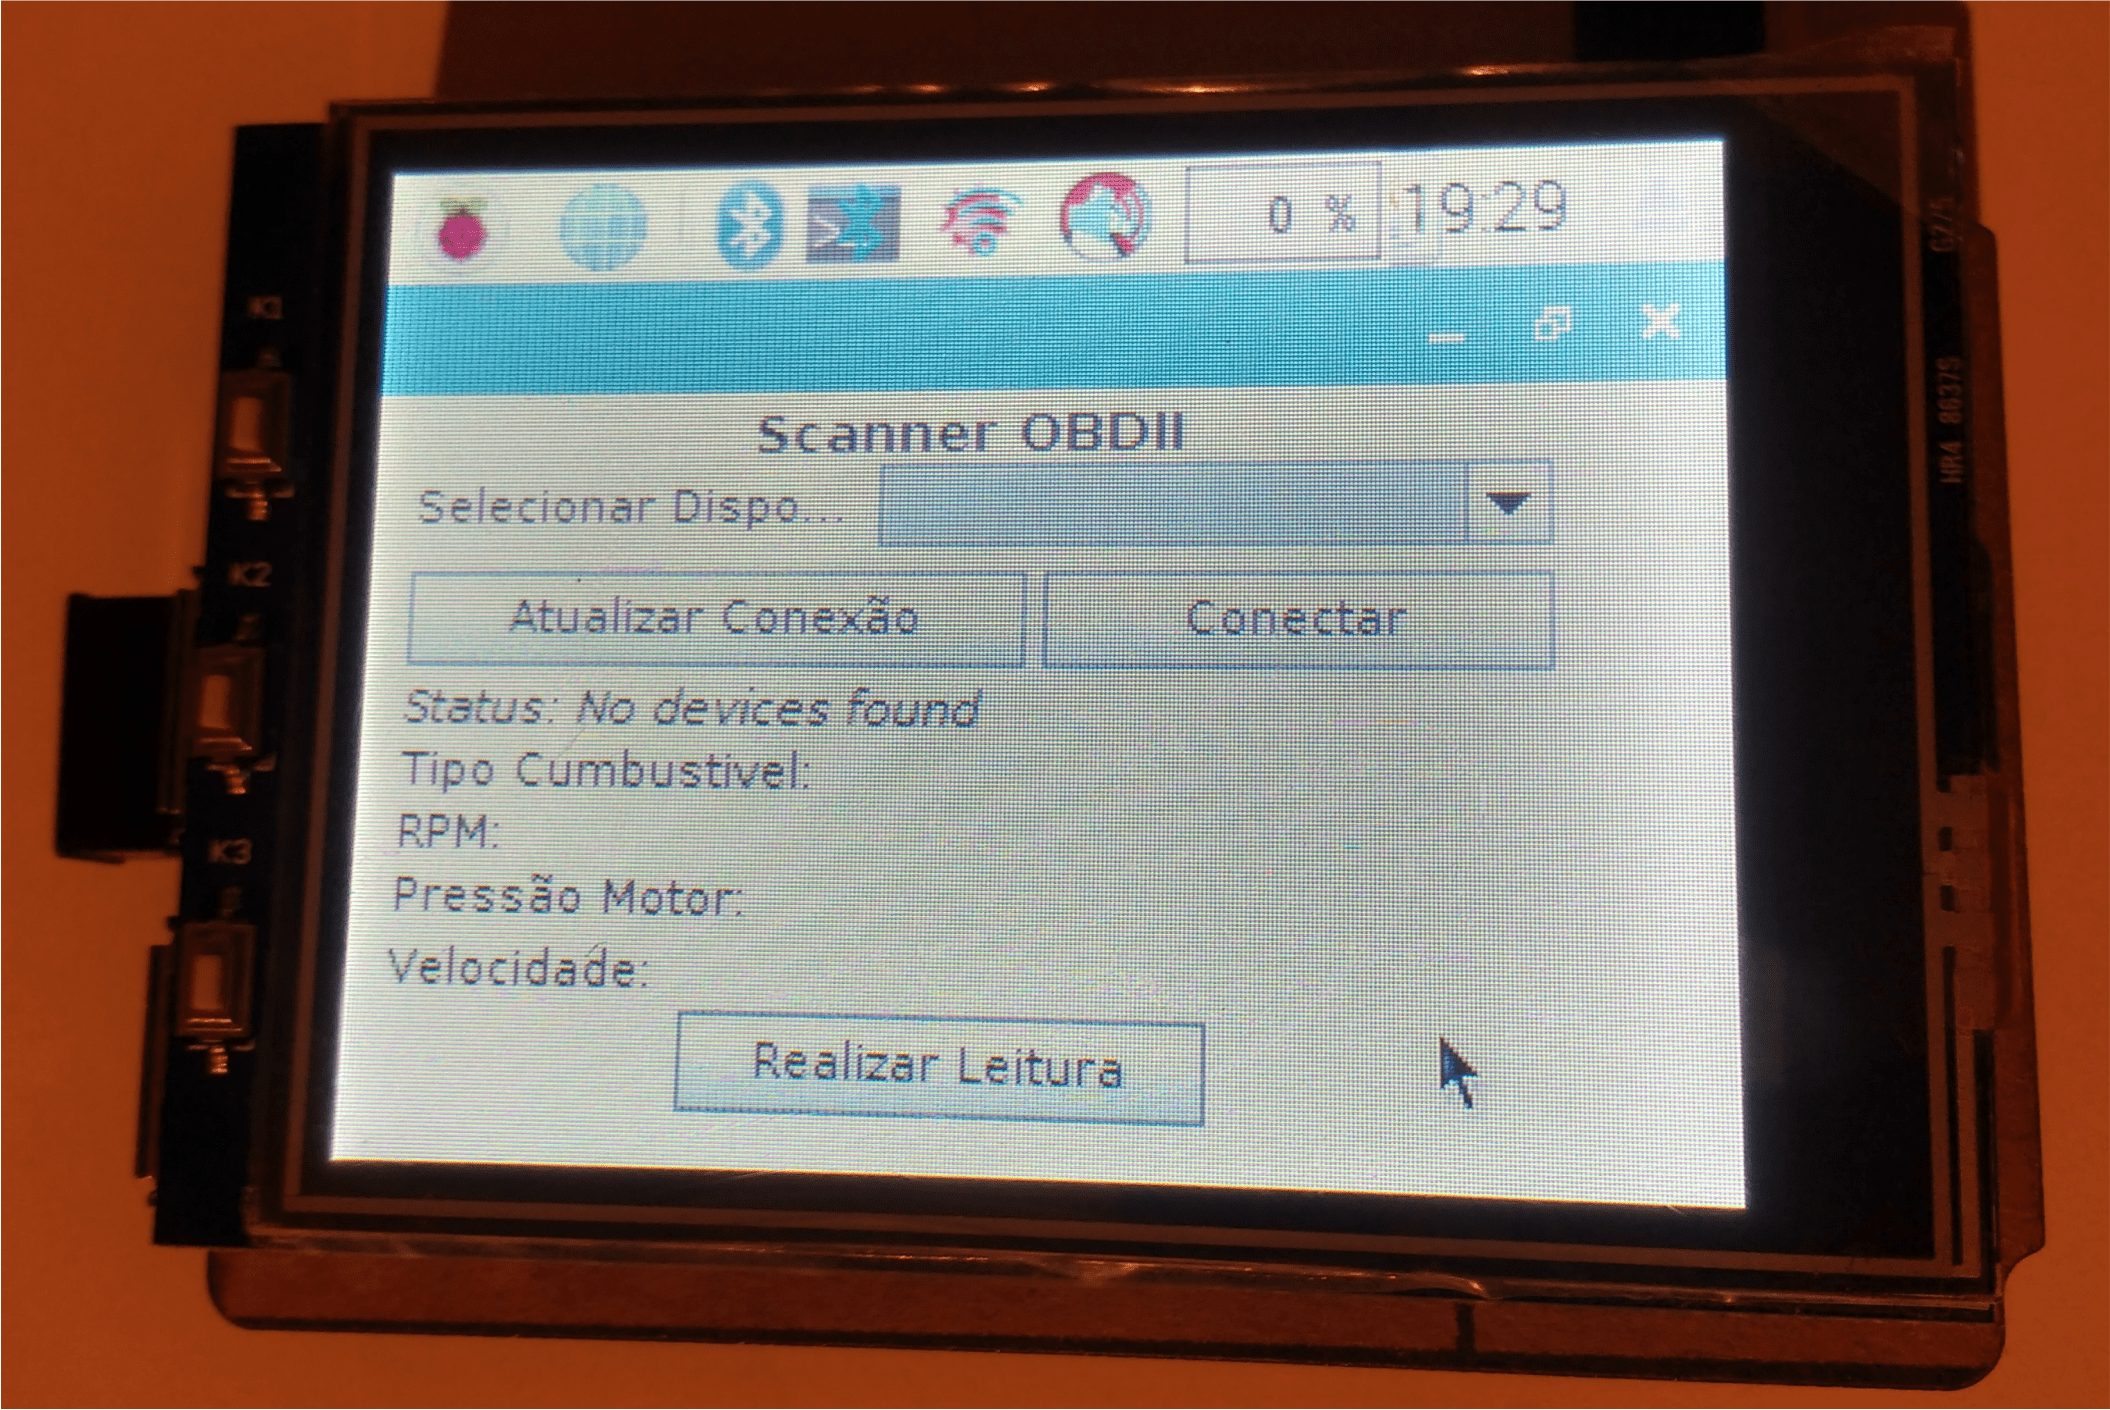
\includegraphics[scale=.15]{imagens/sistemaRodandoRaspberry-min.png}}\\
\makebox[\width]{Fonte: produzido pelo autor} \label{Fig:raspberry_sistema}
\end{figure}

\section{INTEGRAÇÃO DA APLICAÇÃO COM SERVIÇO DE COMPUTAÇÃO EM NUVEM}
Primeiramente foi feita uma análise da arquitetura que o servidor deveria possuir além de levantar quais serviços e software seriam necessários para garantir o funcionamento do sistema na web. Baseando-se nestas informações, foi adquirido um servidor do tipo \textit{Elastic Compute Cloud (EC2)} da Amazon, pertencente à categoria t2.micro, contendo 1Gb de memória RAM, processador Intel Xeon de 2.5GHz e 8Gb de armazenamento do tipo \textit{Elastic Block Store (EBS)}, rodando o sistema operacional Ubuntu \textit{Server} 16.04 LTS. Esta categoria de servidor permite o uso por um ano de forma gratuita. O \textit{EC2}, segundo a \citeonline{amazonec2}, é um \textit{web service} que disponibiliza capacidade computacional segura e redimensionável na nuvem. O \textit{EBS} disponibiliza volumes de armazenamento para uso com instâncias de servidores do tipo \textit{EC2} \nocite{amazonebs}.

\subsection{\textbf{Instalação e configuração da base de dados na nuvem}}
Depois de feita a aquisição do servidor, a próxima etapa foi instalar e configurar um serviço de banco de dados. Para esta situação foi escolhido o MongoDB, que é um banco de dados não relacional baseado em documentos \textit{JSON} \cite{mongodbwhatis}. Este banco possui um esquema de dados flexível, permitindo o mapeamento de um documento para uma entidade ou objeto. Cada documento é armazenado dentro de uma coleção do banco. De acordo com o manual do \citeonline{mongodbdatamodeling}, os modelos de dados desnormalizados permitem que as aplicações alterem a estrutura dos documentos contidos nas coleções durante o armazenamento de dados realizando apenas uma única operação no banco de dados sem se preocupar com a sua remodelagem.

Logo após a instalação do banco, foi criado uma base de dados no MongoDB com o nome \textit{car\_monitor}, e dentro desta base, foi criado uma coleção com o nome \textit{reading\_sensors}. Esta coleção armazenará todos os dados do veículo que foram lidos pelo \textit{Raspberry Pi}. A Figura \ref{Fig:base_dados} representa a estrutura do banco de dados que será responsável por armazenar as informações.

\begin{figure}[!ht]
\centering
\caption{Foto da estrutura do banco de dados.} 
{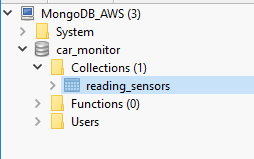
\includegraphics[scale=1.5]{imagens/baseDadosBanco.png}}\\
\makebox[\width]{Fonte: produzido pelo autor} \label{Fig:base_dados}
\end{figure}

\subsection{\textbf{Integração do software com a base de dados}}
Para a integração do software com a base de dados foi necessário instalar as seguintes dependências do MongoDB no projeto: \textit{mongodb-driver}, \textit{mongodb-driver-core} e \textit{bson}, todas na versão 3.5. Para manipular as informações no banco de dados pelo software, foi decidido seguir o modelo \textit{Data Access Object (DAO)}. Segundo a definição de \apudonline{deepak}{medeirosdao}, o padrão \textit{DAO} abstrai e encapsula todos os acessos ao banco de dados, gerenciando a conexão com a base para obter e armazenar as informações. Para implementar este padrão, foi necessário alterar a estrutura do projeto, com a criação de 3 pacotes adicionais: o pacote \textit{dao}, o pacote \textit{database} e o pacote \textit{models}. A Figura \ref{Fig:diagrama_classe_novo} mostra a nova estrutura de pacotes e a Figura \ref{Fig:diagrama_mvc_dao} exibe a representação dos padrões utilizados no projeto baseado nos pacotes implementados.

\begin{figure}[!ht]
\centering
\caption{Diagrama de pacote exibindo a nova estrutura de pacotes do projeto com as respectivas classes.} 
{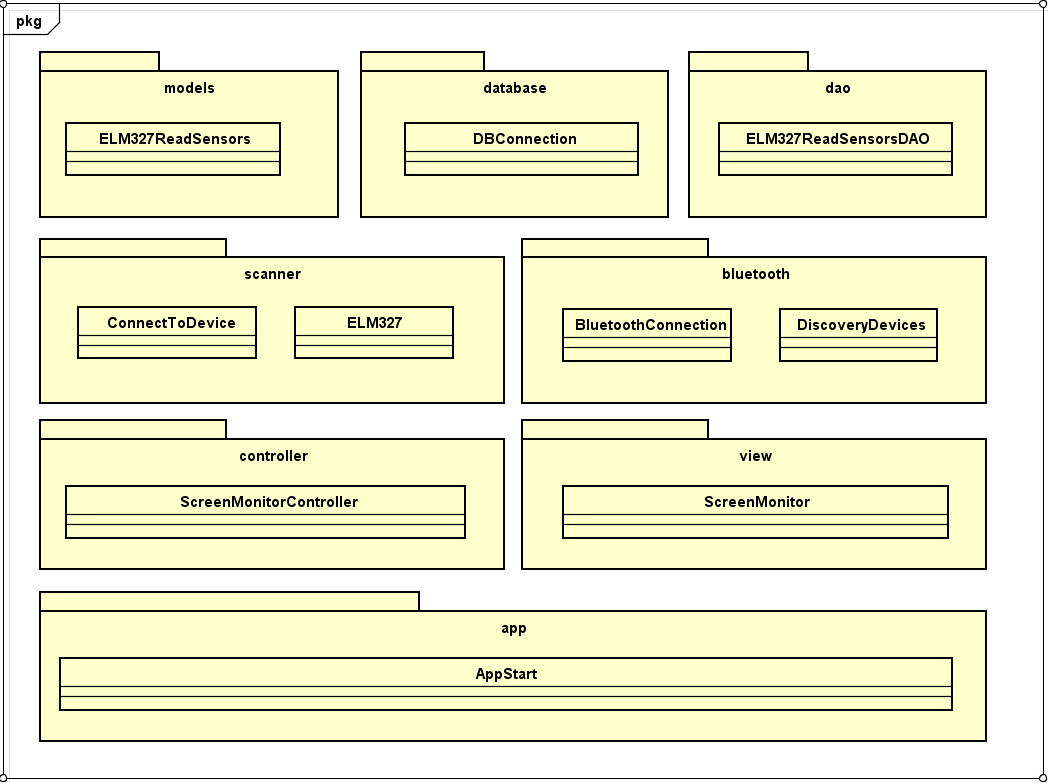
\includegraphics[scale=.44]{imagens/estruturacaoPacotesNovo.png}}\\
\makebox[\width]{Fonte: produzido pelo autor} \label{Fig:diagrama_classe_novo}
\end{figure}

\begin{figure}[!ht]
\centering
\caption{Representação da arquitetura \textit{MVC} com o padrão \textit{DAO} do projeto.} 
{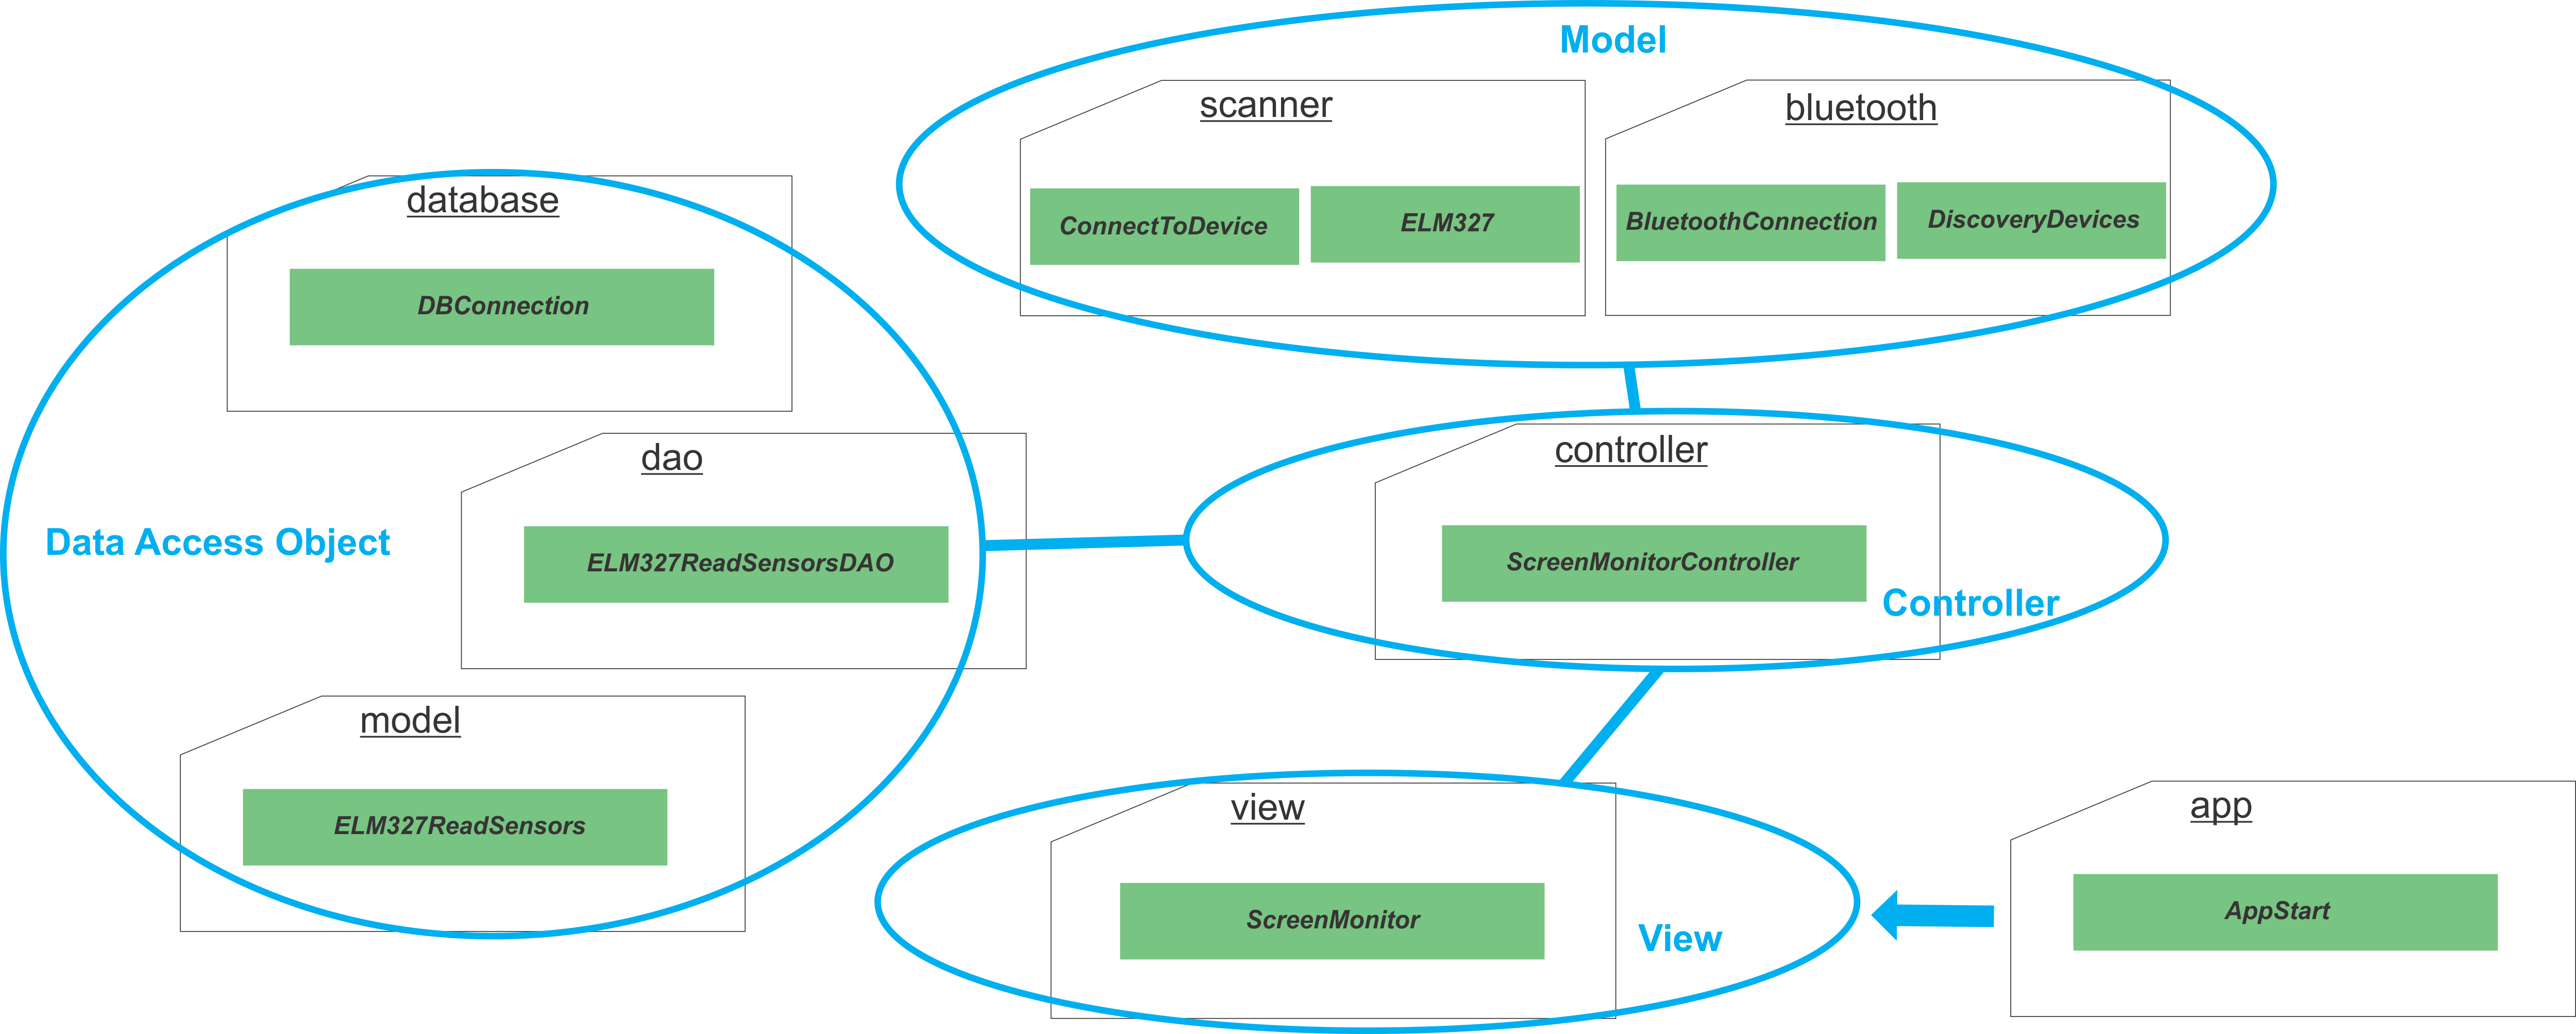
\includegraphics[scale=.38]{imagens/diagramaMvcDao.png}}\\
\makebox[\width]{Fonte: produzido pelo autor} \label{Fig:diagrama_mvc_dao}
\end{figure}

O pacote \textit{model} contém a classe modelo \textit{ELM327ReadSensors} (Figura \ref{Fig:elm327_read_sensors}), que será utilizada para a criação de objetos que armazenarão todas as informações que foram lidas do veículo. Esta classe possui os campos do tipo \textit{string} referentes à estas informações, que são: modeloCarro, chassiCarro, rpm, velocidade, pressaoCombustivel e tipoCombustivel.

\begin{figure}[!ht]
\centering
\caption{Foto da classe \textit{ELM327ReadSensors}.} 
{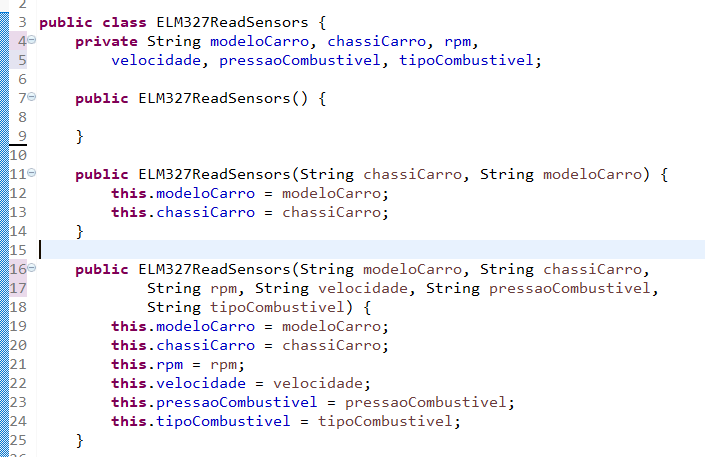
\includegraphics[scale=.66]{imagens/pacoteModel-ELM327ReadSensors.png}}\\
\makebox[\width]{Fonte: produzido pelo autor} \label{Fig:elm327_read_sensors}
\end{figure}

Analisando o pacote \textit{database}, ele traz a classe \textit{DBConnection} (Figura \ref{Fig:db_connection}) que é responsável por criar a conexão com o banco de dados na nuvem. Esta classe contém o método estático \textit{getConnection} que retorna um objeto do tipo \textit{MongoDatabase}, pertencente à biblioteca \textit{mongodb-driver}.

\begin{figure}[!ht]
\centering
\caption{Foto da classe \textit{DBConnection}.} 
{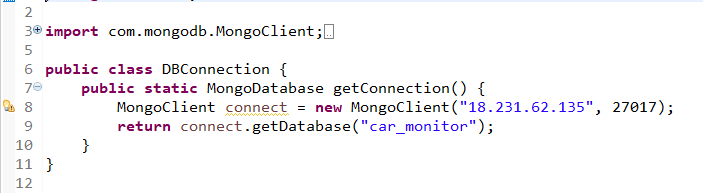
\includegraphics[scale=.66]{imagens/pacoteDatabase-DBConnection.png}}\\
\makebox[\width]{Fonte: produzido pelo autor} \label{Fig:db_connection}
\end{figure}

No pacote \textit{dao}, existe a classe \textit{ELM327ReadSensorsDAO} (Figura \ref{Fig:elm327_read_sensors_dao}), que implementa o padrão \textit{DAO}. Esta classe abstrai o acesso ao banco de dados, fornecendo um método para inserção chamada \textit{insertDB}, que recebe como parâmetro um objeto do tipo \textit{ELM327ReadSensors}. Este método é responsável por receber este objeto e estruturá-lo em um outro objeto no formato \textit{BSON} para ser inserido no banco de dados. Os dados contidos no MongoDB são documentos \textit{JSON} codificados, conhecidos como \textit{BSON} \cite{mongodbjsonbson}.

\begin{figure}[!ht]
\centering
\caption{Foto da classe \textit{ELM327ReadSensorsDAO}.} 
{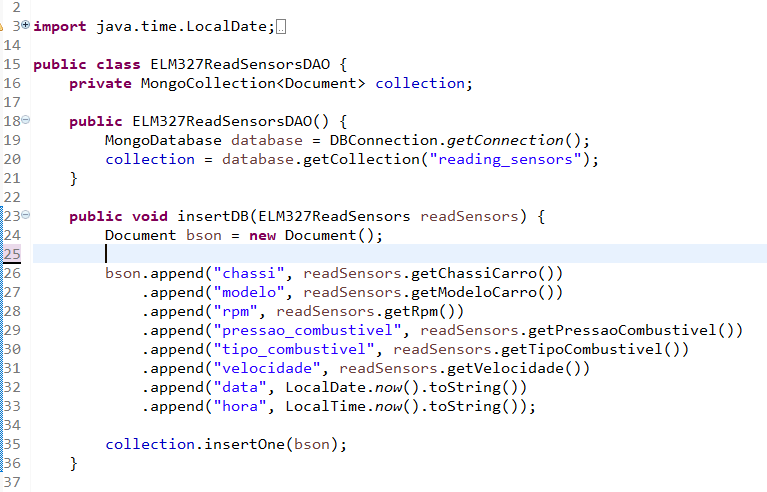
\includegraphics[scale=.66]{imagens/pacoteDao-ELM327ReadSensorsDAO.png}}\\
\makebox[\width]{Fonte: produzido pelo autor} \label{Fig:elm327_read_sensors_dao}
\end{figure}

Para permitir o upload dos dados na nuvem utilizando o \textit{Raspberry Pi}, foi levantado a necessidade de utilizar uma rede móvel 4G. Desta forma, seria possível conectar o software com o MongoDB localizado em uma instância da Amazon na nuvem.

\subsection{\textbf{Instalação e criação do \textit{web service}}}
Depois de integrado o software com o banco de dados, foi necessário criar um \textit{web service} que seria responsável por realizar as consultas no banco e disponibilizá-las para alguma outra aplicação poder consumir estas informações. Baseado nesta definição, foi escolhido a plataforma Node.js na versão 6.11 para a criação do \textit{web service} utilizando a linguagem \textit{JavaScript}. Segundo o \citeonline{w3schools}, o Node.js é uma plataforma para servidor de código aberto que utiliza a linguagem \textit{JavaScript} para as aplicações de \textit{web service}, permitindo a manipulação de informações no \textit{backend}.

Foi necessário a instalação de três pacotes do Node.js para a criação do \textit{web service}: o pacote \textit{express}, responsável pela abstração das rotas, o pacote \textit{body-parser} responsável por efetuar as conversões \textit{JSON} e o pacote \textit{mongoose}, responsável por mapear os objetos do MongoDB. O \textit{web service} foi implementado apenas para requisições HTTP do tipo \textit{GET} na rota \textit{‘/collection’}. Desta maneira, qualquer aplicação que fazer uma solicitação do tipo \textit{GET} para esta rota, será chamado uma função no \textit{web service} (Figura \ref{Fig:get_collection}) que é responsável por realizar a consulta no banco de dados e retornar os valores encontrados em formato de uma lista de objetos \textit{JSON} respondendo à requisição.

\begin{figure}[!ht]
\centering
\caption{Foto do método js responsável por responder a solicitações \textit{GET} na rota \textit{'/collection'}.} 
{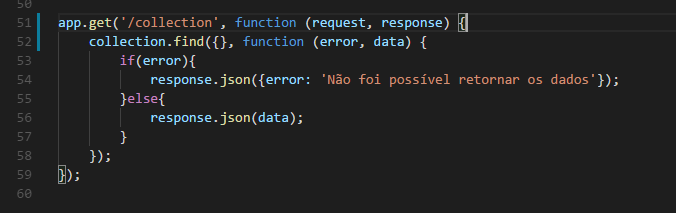
\includegraphics[scale=.66]{imagens/GET-collection_webservice.png}}\\
\makebox[\width]{Fonte: produzido pelo autor} \label{Fig:get_collection}
\end{figure}

\subsection{\textbf{Instalação e configuração do servidor web e criação da página}}
Após concluída a etapa anterior, seria preciso instalar um servidor web para hospedar a página que iria consumir os dados disponibilizados pelo \textit{web service}. Foi escolhido o servidor Apache para esta finalidade. As configurações padrão do servidor Apache foram mantidas, pois não haveria necessidade de alterá-las nesta situação.

O desenvolvimento da página web foi feito utilizando-se as tecnologias HTML, \textit{JQuery} e \textit{Bootstrap}. A função desta página é simplesmente consumir as informações disponíveis no \textit{web service}, não possuindo nenhuma outra funcionalidade específica. A página contém um componente de seleção, que permite escolher o tipo de filtro para exibir os resultados. Logo abaixo contém o campo de entrada que permite inserir o valor da informação que se deseja filtrar. A Figura \ref{Fig:input_fitros} apresenta os componentes de filtro mencionados acima.

\begin{figure}[!ht]
\centering
\caption{Foto dos elementos de filtro da página.} 
{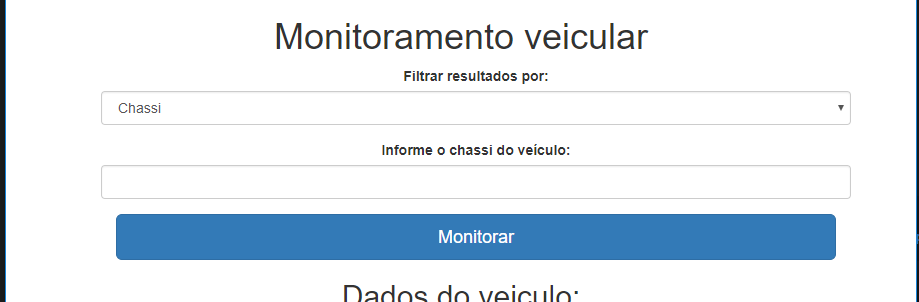
\includegraphics[scale=.62]{imagens/paginaweb_inputs.png}}\\
\makebox[\width]{Fonte: produzido pelo autor} \label{Fig:input_fitros}
\end{figure}

Após preenchido o valor, existe um botão chamado monitorar, que ao acionado, faz a requisição \textit{GET} via \textit{AJAX} (Figura \ref{Fig:requisicao_ajax}) para o \textit{web service} e retorna os valores na tabela de acordo com o filtro informado.
Por fim, a Figura \ref{Fig:arquitetura_projeto} mostra toda a integração do sistema com a nuvem, representando as trocas de dados e comunicação entre diferentes serviços.

\begin{figure}[!ht]
\centering
\caption{Foto do método \textit{JQuery} responsável pelo \textit{AJAX}.} 
{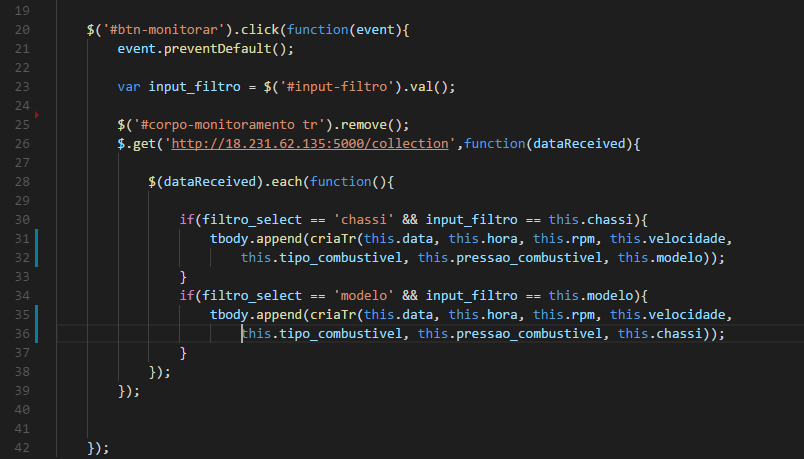
\includegraphics[scale=.64]{imagens/requisicaoAjax.png}}\\
\makebox[\width]{Fonte: produzido pelo autor} \label{Fig:requisicao_ajax}
\end{figure}

\begin{figure}[!ht]
\centering
\caption{Diagrama representando a comunicação do sistema com a nuvem.} 
{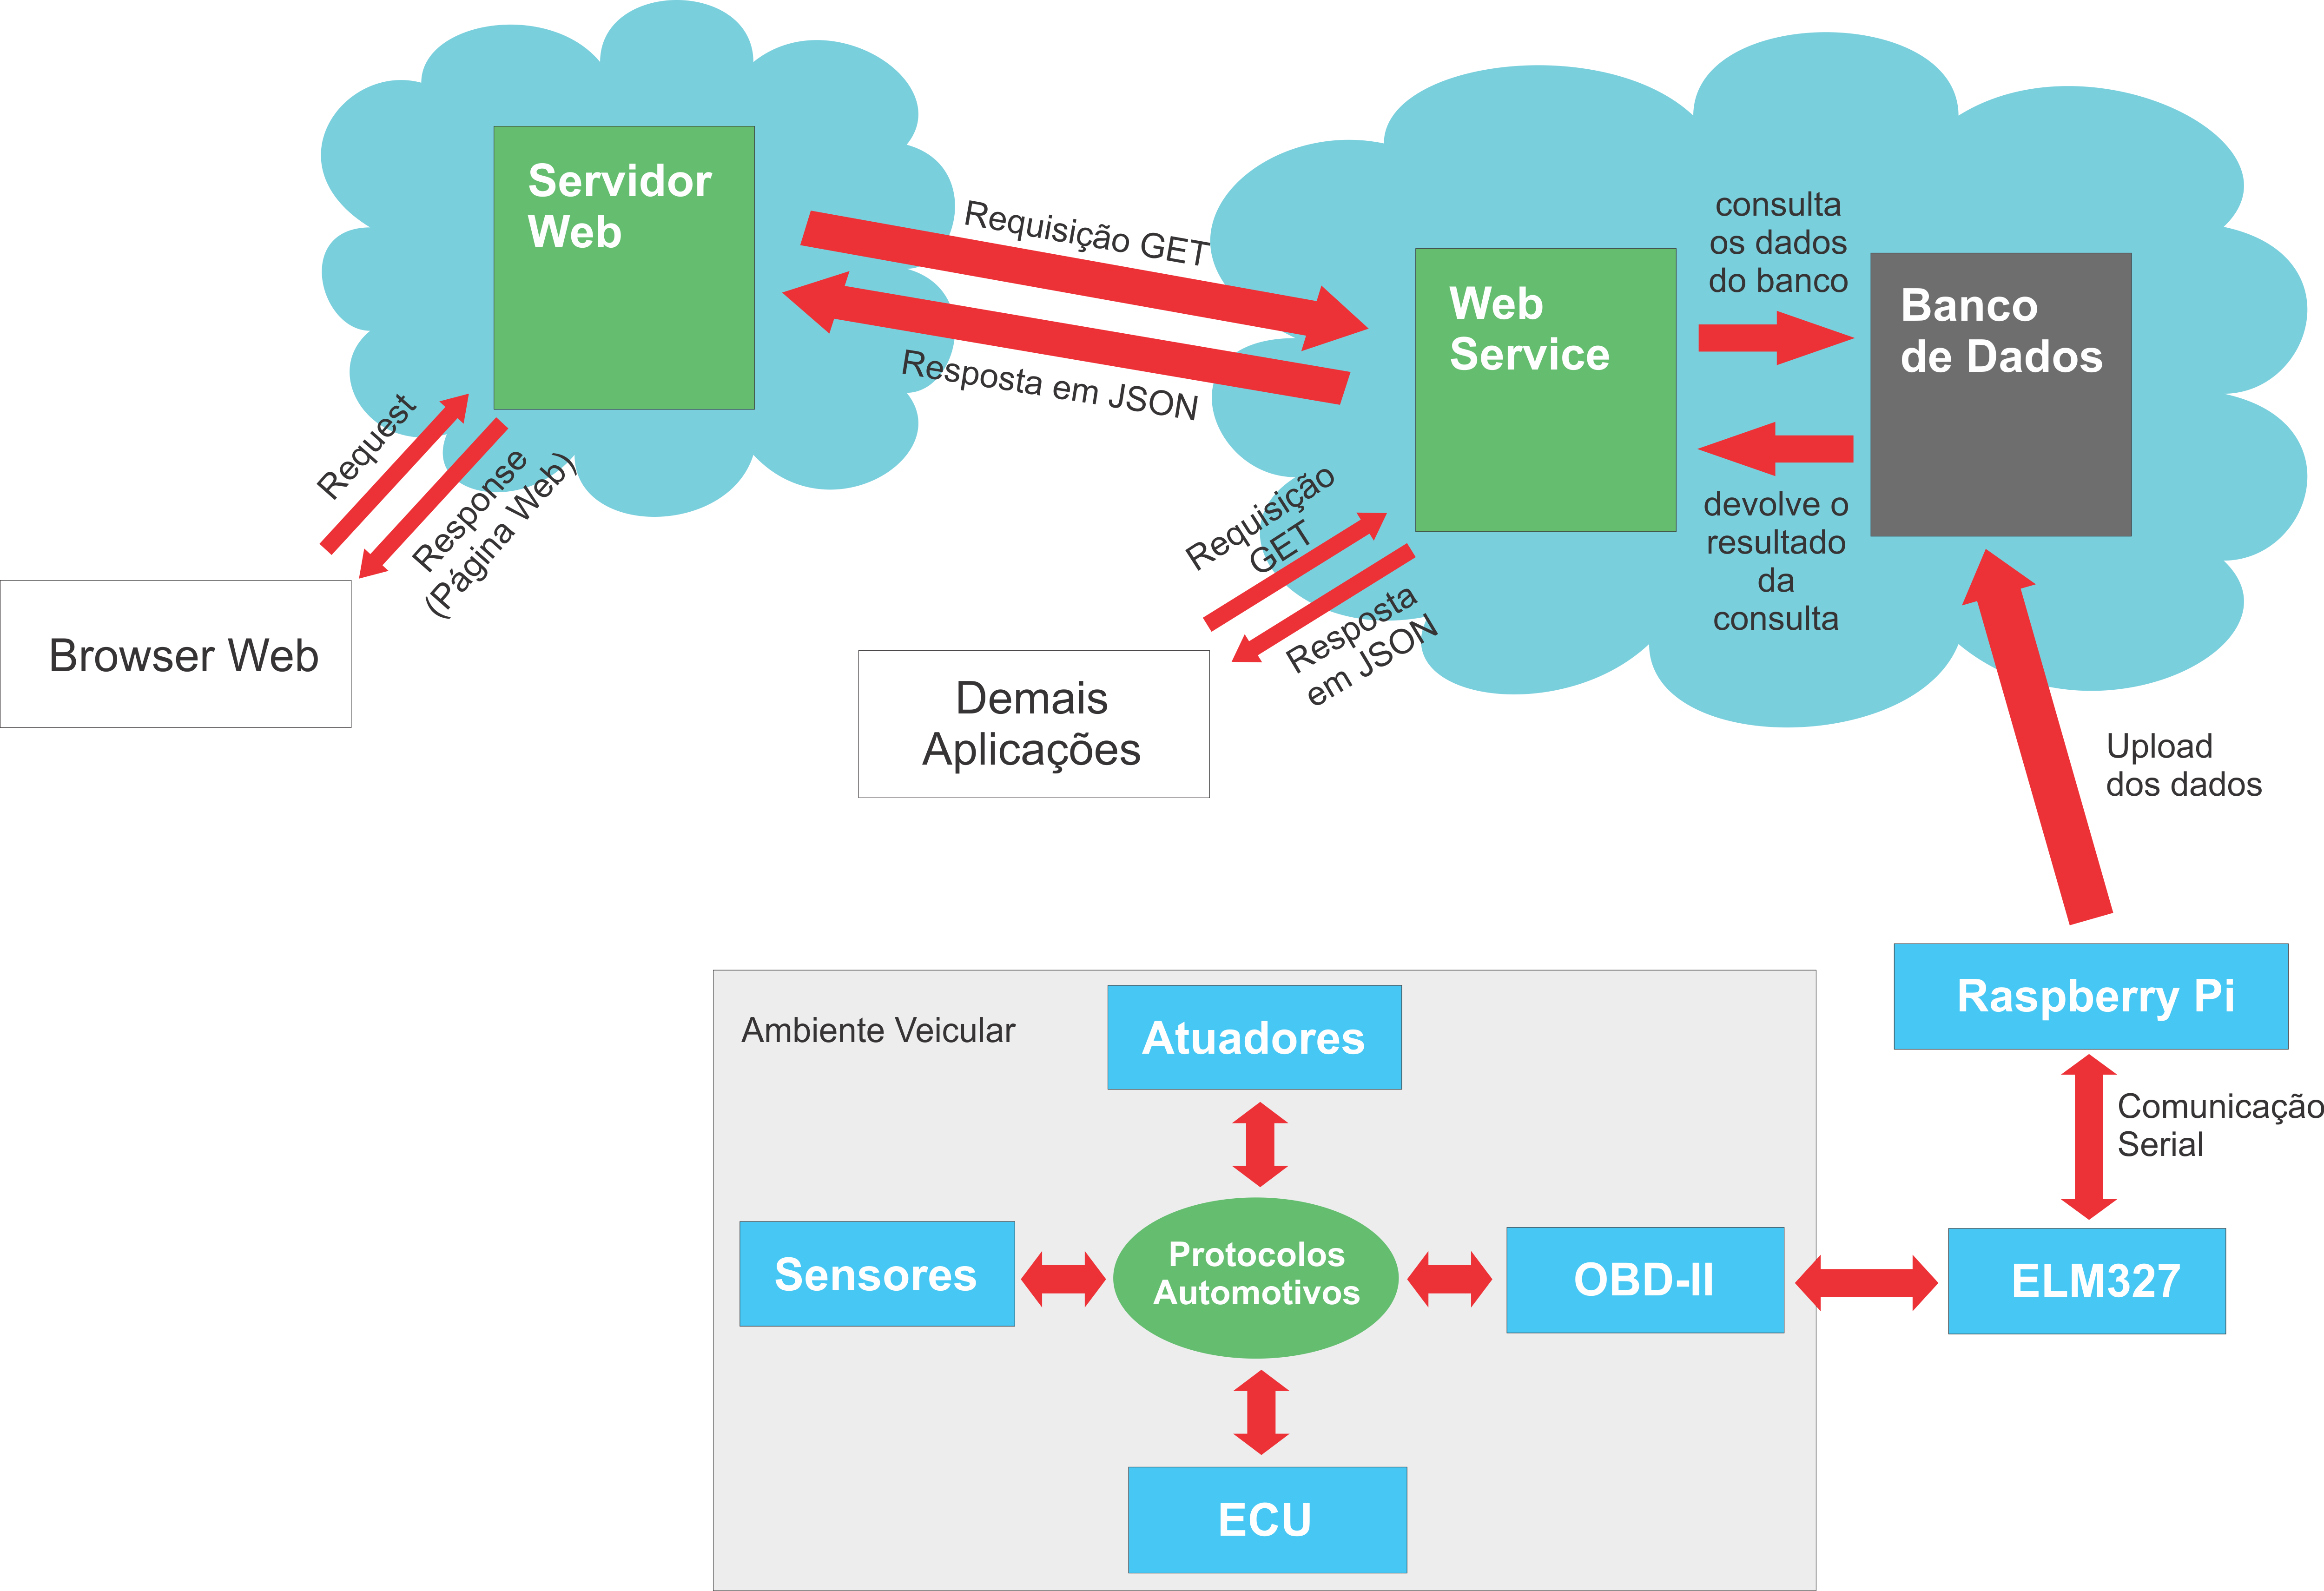
\includegraphics[scale=.38]{imagens/arquiteturaRedeVeicularELM327Nuvem.png}}\\
\makebox[\width]{Fonte: produzido pelo autor} \label{Fig:arquitetura_projeto}
\end{figure}

\chapter{TESTES E AVALIAÇÃO DOS RESULTADOS}\label{CAP6}
Durante o desenvolvimento do sistema como um todo, desde a sua fase local de desenvolvimento do software até a integração com os serviços da computação em nuvem, foram feitos diversos testes para garantir que as funcionalidades básicas estipuladas no início estavam sendo atendidas. Desta forma, será abordado nesta seção como foram realizadas cada etapa dos testes, e os principais resultados obtidos.

\section{TESTE DO SOFTWARE DE LEITURA}
Depois de desenvolvido o software, foram realizados os testes de funcionalidade no ambiente de desenvolvimento (notebook) para analisar se o funcionamento estava conforme o esperado. Nesta etapa, verificou-se que algumas leituras obtidas do ELM327 estavam retornando valores que não condiziam com a realidade. Contudo, estes valores eram tratados pela biblioteca obd-java-api, disparando uma \textit{exception} da própria biblioteca referente ao valor retornado. Baseado no resultado deste teste, houve três hipóteses que foram levantadas: a primeira, possivelmente o PID referente à leitura não era suportado (ou não foi implementado) pelo veículo ou protocolo utilizado; a segunda, possivelmente por questões de segurança, o próprio sistema do veículo negou a requisição para o PID; ou ainda, poderia haver a possibilidade do dispositivo estar retornando algum dado inválido, podendo ser lixo de memória ou \textit{buffer}.

Depois de feito a análise do problema, foi realizado mais testes direcionados à exploração desta falha visando uma possível correção. Foi necessário também consultar a documentação do dispositivo ELM327 para entender como ele trabalhava com as solicitações. Desta forma, foi descoberto que o dispositivo é capaz de retransmitir a leitura anterior, semelhante a um eco. Isso é possível pois o dispositivo contém uma pequena memória de \textit{buffer} que armazena o último comando enviado para o dispositivo. Baseando-se nestas informações coletadas, foi decidido implementar o método \textit{clearBuffer} na classe ELM327, contendo alguns comandos ‘AT’ que eram responsáveis por apagar o eco e reiniciar a comunicação, para garantir que o \textit{buffer} estivesse limpo para a nova leitura.

Após realizar a alteração proposta, foi observado que algumas das leituras que antes retornavam uma \textit{exception} estavam agora retornando valores válidos e formatados segundo a implementação da biblioteca. Entretanto, algumas leituras ainda continuaram a retornar as \textit{exceptions}. Baseando-se nestas observações, para as leituras que foram possíveis após a alteração mencionada, uma explicação aceitável seria a probabilidade do \textit{buffer} estar sujo. Para explicar as outras leituras que persistiram com o problema mencionado, poderia ser uma das duas primeiras hipóteses levantadas no início.

Além da questão levantada acima, observou-se também certa lentidão durante a inicialização do software e durante a realização de algumas leituras. Inicialmente foi levantado a hipótese de que a comunicação \textit{bluetooth} que estava causando a lentidão, entretanto, quando foi implementado a mesma lógica pelo console, notou-se que a execução dele foi mais rápido. Baseado neste teste, concluiu-se que a implementação contendo a interface gráfica estava deixando a execução do software mais lenta. Entretanto, apesar desta análise e conclusão, foi mantida a interface do sistema.

\section{TESTE DE INTEGRAÇÃO DO SOFTWARE COM O \textit{RASPBERRY PI}}
Depois de preparado o ambiente do \textit{Raspberry Pi}, foi executado o software no dispositivo para análise e testes. Conforme já apresentado na metodologia, foi identificado algumas incompatibilidades que foram solucionadas logo na sequência. Contudo, depois das alterações, notou-se que o software foi executado mais rápido que comparado à primeira execução no ambiente de desenvolvimento, mas ainda demorava algum tempo em alguns momentos da execução. Analisando-se o resultado dos testes, foi levantado a hipótese da lentidão estar sendo causada pelo fato do software estar rodando no dispositivo através da máquina virtual do Java \textit{(Java Virtual Machine – JVM)}, combinado com a renderização da interface.

A fim de tornar a execução mais rápida, foi feita uma análise técnica para estudar a viabilidade de migração do software para a linguagem \textit{Python}. Além do \textit{Raspberry} suportar scripts \textit{Python}, \citeonline{richardsonwallace} ainda afirmam que esta linguagem tende a ser mais rápida pelo fato de ser interpretada. Durante a análise, foi encontrado uma biblioteca em \textit{Python} que trazia diversas funções que permitiam a comunicação com o ELM327, assim como a biblioteca para Java obd-java-api. Esta biblioteca para \textit{Python} foi encontrada em http://python-obd.readthedocs.io/en/latest/, junto com a documentação explicando as principais funções presentes nela. Apesar desta alternativa parecer, em primeiro momento, uma solução viável, houveram alguns contratempos, que levaram a permanência do software na linguagem Java. Uma das dificuldades que tornou inviável a mudança foi atrelado ao trabalho que levaria reestruturar todo o software na nova linguagem, considerando que todas as partes funcionais já estavam prontas em Java. Outro fato que determinou a inviabilidade foi relacionado ao tempo que seria necessário para aprendizado do \textit{Python}, desconsiderando ainda a curva de aprendizagem que poderia existir ao implementar a biblioteca ou integrar a outras tecnologias da linguagem.

\section{TESTES DE INTEGRAÇÃO DA APLICAÇÃO COM A COMPUTAÇÃO EM NUVEM}
Após finalizado toda a parte de integração com os recursos da computação em nuvem, desde banco de dados até o \textit{web service}, foram realizados diversos testes para garantir a comunicação entre os sistemas. Nesta fase, não houve dificuldades e todo o sistema se comunicou conforme o esperado. Para garantir a comunicação do software instalado no \textit{Raspberry Pi} com o banco de dados na nuvem, foi utilizado uma infraestrutura de rede móvel 4G, conforme já abordado anteriormente. O teste foi realizado com o veículo em movimento, e foi notado que durante a execução, a única limitação que foi observada é que ao entrar em uma região sem cobertura 4G, o sistema não fazia upload das informações, o que resultava em perda dos dados que foram coletados. Contudo, toda informação enviada ao banco de dados era disponibilizado pelo \textit{web service} em formato de uma lista de objetos \textit{JSON} (Figura \ref{Fig:json_retorno_web}) para ser consumido por outra aplicação.

\begin{figure}[!ht]
\centering
\caption{Foto dos objetos \textit{JSON} disponibilizados pelo \textit{web service}.} 
{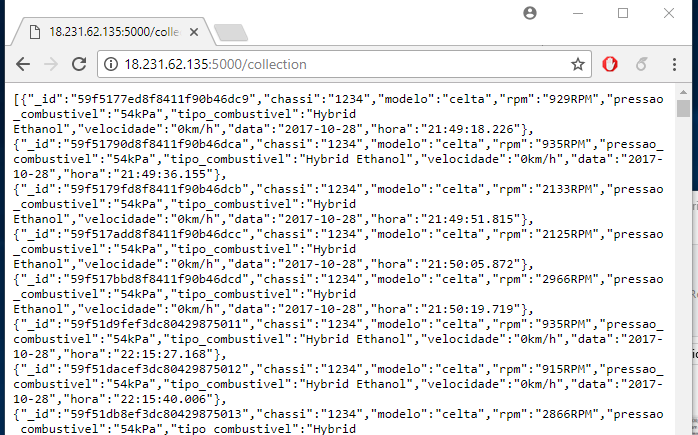
\includegraphics[scale=.68]{imagens/JSON_retornoWebservice.png}}\\
\makebox[\width]{Fonte: produzido pelo autor} \label{Fig:json_retorno_web}
\end{figure}

Por fim, foi testado com sucesso o consumo dos dados por meio de uma página web (Figura \ref{Fig:pagina_web_tabela_dados}), através de requisições utilizando o \textit{AJAX} do \textit{JQuery} pelo \textit{frontend}.

\begin{figure}[!ht]
\centering
\caption{Foto da página web estruturando em uma tabela os dados \textit{JSON}.} 
{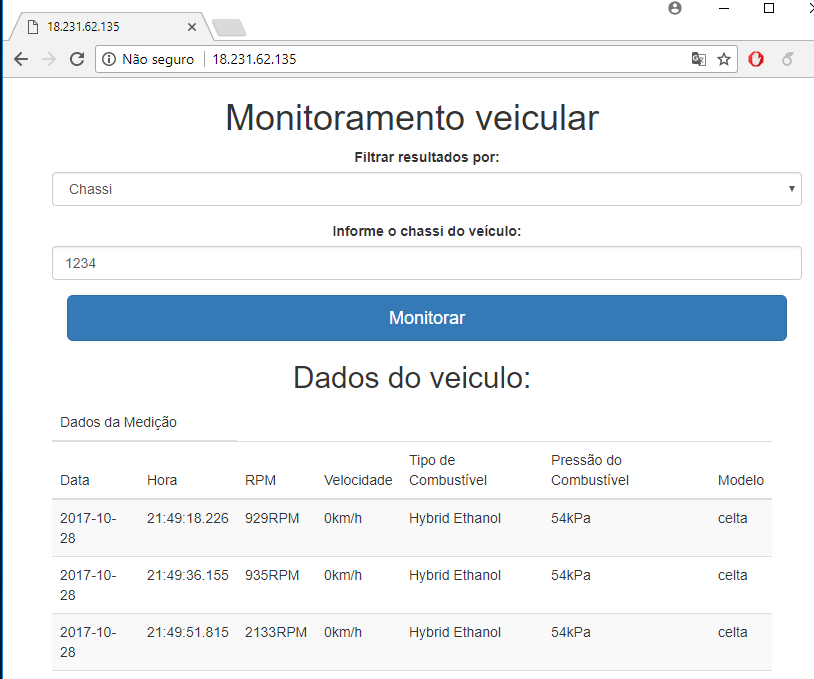
\includegraphics[scale=.68]{imagens/paginaweb_tabelaDados.png}}\\
\makebox[\width]{Fonte: produzido pelo autor} \label{Fig:pagina_web_tabela_dados}
\end{figure}
\chapter{CONCLUSÕES}\label{CAP7}
Este trabalho mostrou um estudo detalhado da arquitetura presente nos sistemas embarcados automotivos e também a forma com que estes sistemas se comunicam, apresentando as categorias e protocolos utilizados, e como o sistema é dividido. Neste estudo também foi observada a limitação de informações disponibilizadas pelas montadoras sobre os sistemas eletrônicos presentes em seus automóveis. Foi visto também que é fundamental a realização do diagnóstico para a prevenção de eventuais problemas, e a importância do estudo de aplicações voltadas ao cenário automotivo, buscando integrá-lo à tecnologia da informação. Na sequência, foram explorados também alguns conceitos de informática que puderam se relacionar diretamente e indiretamente com o ambiente de um automóvel e como esses conceitos poderiam se cruzar, permitindo aplicações possivelmente viáveis aplicadas à internet das coisas.

Com base neste estudo, foi proposto o desenvolvimento de um sistema responsável por ler as informações relacionadas ao funcionamento do automóvel presentes em uma rede veicular, processar os dados e enviá-los a um banco de dados localizado na nuvem, e a partir disso, disponibilizar estas informações para o acesso de eventuais aplicações, buscando colocar em prática os conceitos estudados ao longo do trabalho. Entretanto, apesar do êxito em efetuar a leitura dos dados presentes nos automóveis, não foi possível verificar se a conversão das informações lidas do automóvel foi precisa por faltar parâmetros de comparação autênticos.

\section{PROPOSTA PARA TRABALHOS FUTUROS}
As dificuldades enfrentadas ao longo do percurso deixam margem para a exploração de outros trabalhos relacionados, além desta proposta. Existem alguns ajustes que podem ser aperfeiçoados numa extensão deste projeto.

Um dos pontos de melhoria é relacionado à tela do \textit{Raspberry Pi} que foi adquirida. Notou-se que a tela de 3.2 polegadas era muito pequena para a exibição das informações, o que levou à adaptação da interface para exibição dos dados. Isso resultou na redução de informações que seriam exibidas na tela. Uma possível sugestão seria a utilização de uma tela de 5 polegadas ou maior.

Outro aspecto que também pode ser explorado é a análise da precisão dos valores que foram obtidos do veículo através do software. É importante comparar os valores gerados pelo sistema com os gerados através de \textit{scanners} e outros equipamentos de leitura originais das montadoras. É importante também analisar os valores que são considerados padrões pelas montadoras junto com as variações permitidas, comparando-as com os valores obtidos.

Analisando-se os resultados referentes ao desempenho do sistema, seria possível considerar a reimplementação do software utilizando a linguagem \textit{Python} para fins de estudo e análise de eficiência do algoritmo. Mesmo levantada a hipótese de uma possível otimização com esta linguagem, é necessário colocar em prática para a análise do resultado e confirmação da teoria.

Uma sugestão de melhoria futura do sistema está relacionado com o estudo de políticas de segurança, uma vez que o sistema está totalmente conectado na web, e em sua concepção não foi medido os possíveis riscos e o impacto que poderia gerar. A questão da privacidade dos dados que serão disponibilizados também é um assunto que poderá ser discutido e definido métricas ou ações a serem tomadas para não infringí-la.

Analisando toda a estrutura do trabalho, é possível notar que o sistema poderá gerar grande volume de dados de forma diversificada (indo ao encontro do conceito definido por \citeauthor{chede} de \textit{Big Data}) tendo uma estrutura totalmente escalável e conectada à internet. Desta forma, observando a infraestrutura utilizada, como o uso de tecnologia de baixo custo, a computação em nuvem e o uso de um banco de dados não relacional, torna-se possível uma extensão de estudo por outras áreas que podem se integrar a este trabalho, como envolvendo aplicações de internet das coisas e \textit{Big Data}.

%% ----------------------------------------------------------
\pagestyle{scrplain} 

%% ELEMENTOS POS-TEXTUAIS
\pagestyle{scrplain} 

\postextual

\bibliographystyle{abnt-alf}
\bibliography{bibliografia}
\chapter{ANEXO A}\label{anexoa}

Fazendo uma análise do pacote \textit{bluetooth}, existe a classe \textit{BluetoothConnection} que traz um método estático chamado \textit{getConnectionBluetooth} (Figura \ref{Fig:get_connection_bluetooth}), esperando como parâmetro uma URL de conexão. Este método que tem a responsabilidade de obter uma conexão \textit{bluetooth} devolvendo um objeto do tipo \textit{StreamConnection}, pertencente à biblioteca \textit{BlueCove}. A Classe \textit{DiscoveryDevices} (Figura \ref{Fig:discovery_devices}) implementa a interface \textit{DiscoveryListener}, também pertencente à biblioteca \textit{BlueCove}, que permite a descoberta de dispositivos e serviços. Esta interface fornece quatro métodos para serem implementados: dois para descobrir dispositivos, que são o \textit{deviceDiscovered} (Figura \ref{Fig:device_discovered}) – método que é invocado quando é encontrado um dispositivo durante uma consulta – e o \textit{inquiryCompleted} (Figura \ref{Fig:inquiry_completed}) – método que é chamado quando uma consulta é concluída, e dois para descobrir serviços, que são o \textit{servicesDiscovered} (Figura \ref{Fig:services_discovered}) – são invocados quando os serviços são encontrados durante uma pesquisa por serviços – e o \textit{serviceSearchCompleted} (Figura \ref{Fig:service_search_completed}) – são chamados quando uma pesquisa de serviço foi concluída ou encerrada devido a um erro \cite{bluecovedoc}. Além destes métodos contidos na assinatura da interface, a classe \textit{DiscoveryDevices} também traz o método \textit{discovery} (Figura \ref{Fig:discovery}), responsável por iniciar a descoberta de dispositivos.

\begin{figure}[!ht]
\centering
\caption{Foto do método \textit{getConnectionBluetooth} da classe \textit{BluetoothConnection}.} 
{\includegraphics[scale=.80]{imagens/pacoteBluetooth-BluetoothConnection.PNG}}\\
\makebox[\width]{Fonte: produzido pelo autor} \label{Fig:get_connection_bluetooth}
\end{figure}

\begin{figure}[!ht]
\centering
\caption{Foto da Classe \textit{DiscoveryDevices} implementando a interface \textit{DiscoveryListener}.} 
{\includegraphics[scale=.94]{imagens/pacoteBluetooth-DiscoveryDevices_DiscoveryListener.PNG}}\\
\makebox[\width]{Fonte: produzido pelo autor} \label{Fig:discovery_devices}
\end{figure}

\begin{figure}[!ht]
\centering
\caption{Foto do método \textit{deviceDiscovered} da classe \textit{DiscoveryDevices}.} 
{\includegraphics[scale=.78]{imagens/pacoteBluetooth-DiscoveryDevices_deviceDiscovered.PNG}}\\
\makebox[\width]{Fonte: produzido pelo autor} \label{Fig:device_discovered}
\end{figure}

\begin{figure}[!ht]
\centering
\caption{Foto do método \textit{inquiryCompleted} da classe \textit{DiscoveryDevices}.} 
{\includegraphics[scale=.80]{imagens/pacoteBluetooth-DiscoveryDevices_inquiryCompleted.PNG}}\\
\makebox[\width]{Fonte: produzido pelo autor} \label{Fig:inquiry_completed}
\end{figure}

\begin{figure}[!ht]
\centering
\caption{Foto do método \textit{servicesDiscovered} da classe \textit{DiscoveryDevices}.} 
{\includegraphics[scale=.78]{imagens/pacoteBluetooth-DiscoveryDevices_servicesDiscovered.PNG}}\\
\makebox[\width]{Fonte: produzido pelo autor} \label{Fig:services_discovered}
\end{figure}

\begin{figure}[!ht]
\centering
\caption{Foto do método \textit{serviceSearchCompleted} da classe \textit{DiscoveryDevices}.} 
{\includegraphics[scale=.78]{imagens/pacoteBluetooth-DiscoveryDevices_serviceSearchCompleted.PNG}}\\
\makebox[\width]{Fonte: produzido pelo autor} \label{Fig:service_search_completed}
\end{figure}

\begin{figure}[!ht]
\centering
\caption{Foto do método \textit{discovery} da classe \textit{DiscoveryDevices}.} 
{\includegraphics[scale=.70]{imagens/pacoteBluetooth-DiscoveryDevices_discovery.PNG}}\\
\makebox[\width]{Fonte: produzido pelo autor} \label{Fig:discovery}
\end{figure}

Observando o pacote \textit{scanner}, existe a classe \textit{ConnectToDevice} (Figura \ref{Fig:connect_to_device}) que espera como parâmetro em seu construtor um objeto do tipo \textit{DiscoveryDevices}. Esta classe também possui o método \textit{connectToDevice} (Figura \ref{Fig:connect_connect_to_device}), que espera como parâmetro um índice referente ao dispositivo que se deseja conectar. 

\begin{figure}[!ht]
\centering
\caption{Foto da classe \textit{ConnectToDevice}.} 
{\includegraphics[scale=.80]{imagens/pacoteScanner-ConnectToDevice.PNG}}\\
\makebox[\width]{Fonte: produzido pelo autor} \label{Fig:connect_to_device}
\end{figure}

\begin{figure}[!ht]
\centering
\caption{Foto do método \textit{connectToDevice} da classe \textit{ConnectToDevice}.} 
{\includegraphics[scale=.70]{imagens/pacoteScanner-ConnectToDevice_connectToDevice.PNG}}\\
\makebox[\width]{Fonte: produzido pelo autor} \label{Fig:connect_connect_to_device}
\end{figure}

\end{document}
